\documentclass{article}
\usepackage{times}
\usepackage{graphicx}

% Default margins are too wide all the way around. I reset them here
\setlength{\topmargin}{-.5in}
\setlength{\textheight}{9in}
\setlength{\oddsidemargin}{.125in}
\setlength{\textwidth}{6.25in}
\begin{document}

\title{Tag and Probe results }
\author{Gian Michele}
\date{15 August}

%  const double MuPtBin[nMuPtBin+1] = {0.0,1.5,3.0,4.5,6.0,9.0,20.0,30.0};
%  const double MuEtaBin[nMuEtaBin+1] = {-2.4,-1.5,-0.5,0.5,1.5,2.4};


\maketitle

\begin{figure}
    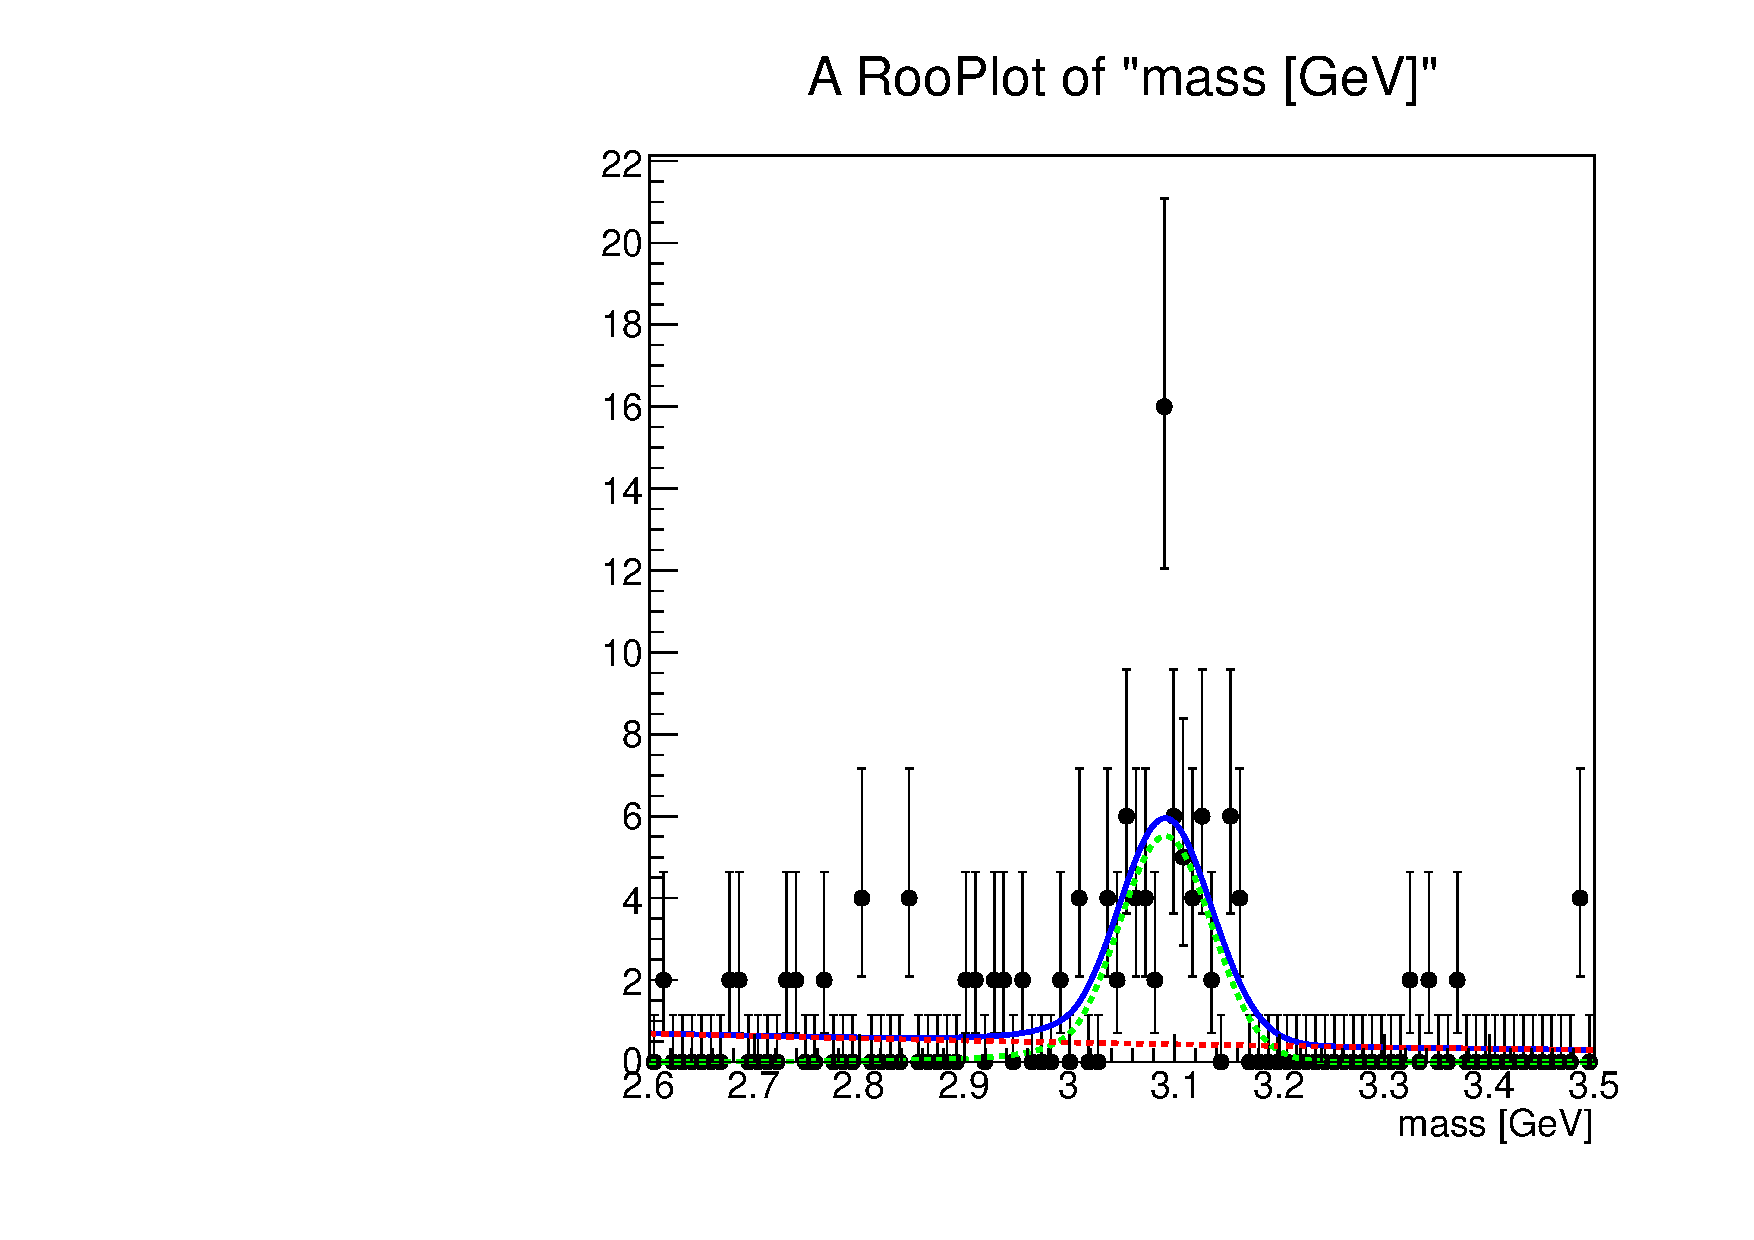
\includegraphics[width=0.25\textwidth]{../PlotsRooFitMC/croofit_trg_pass_0.pdf}
    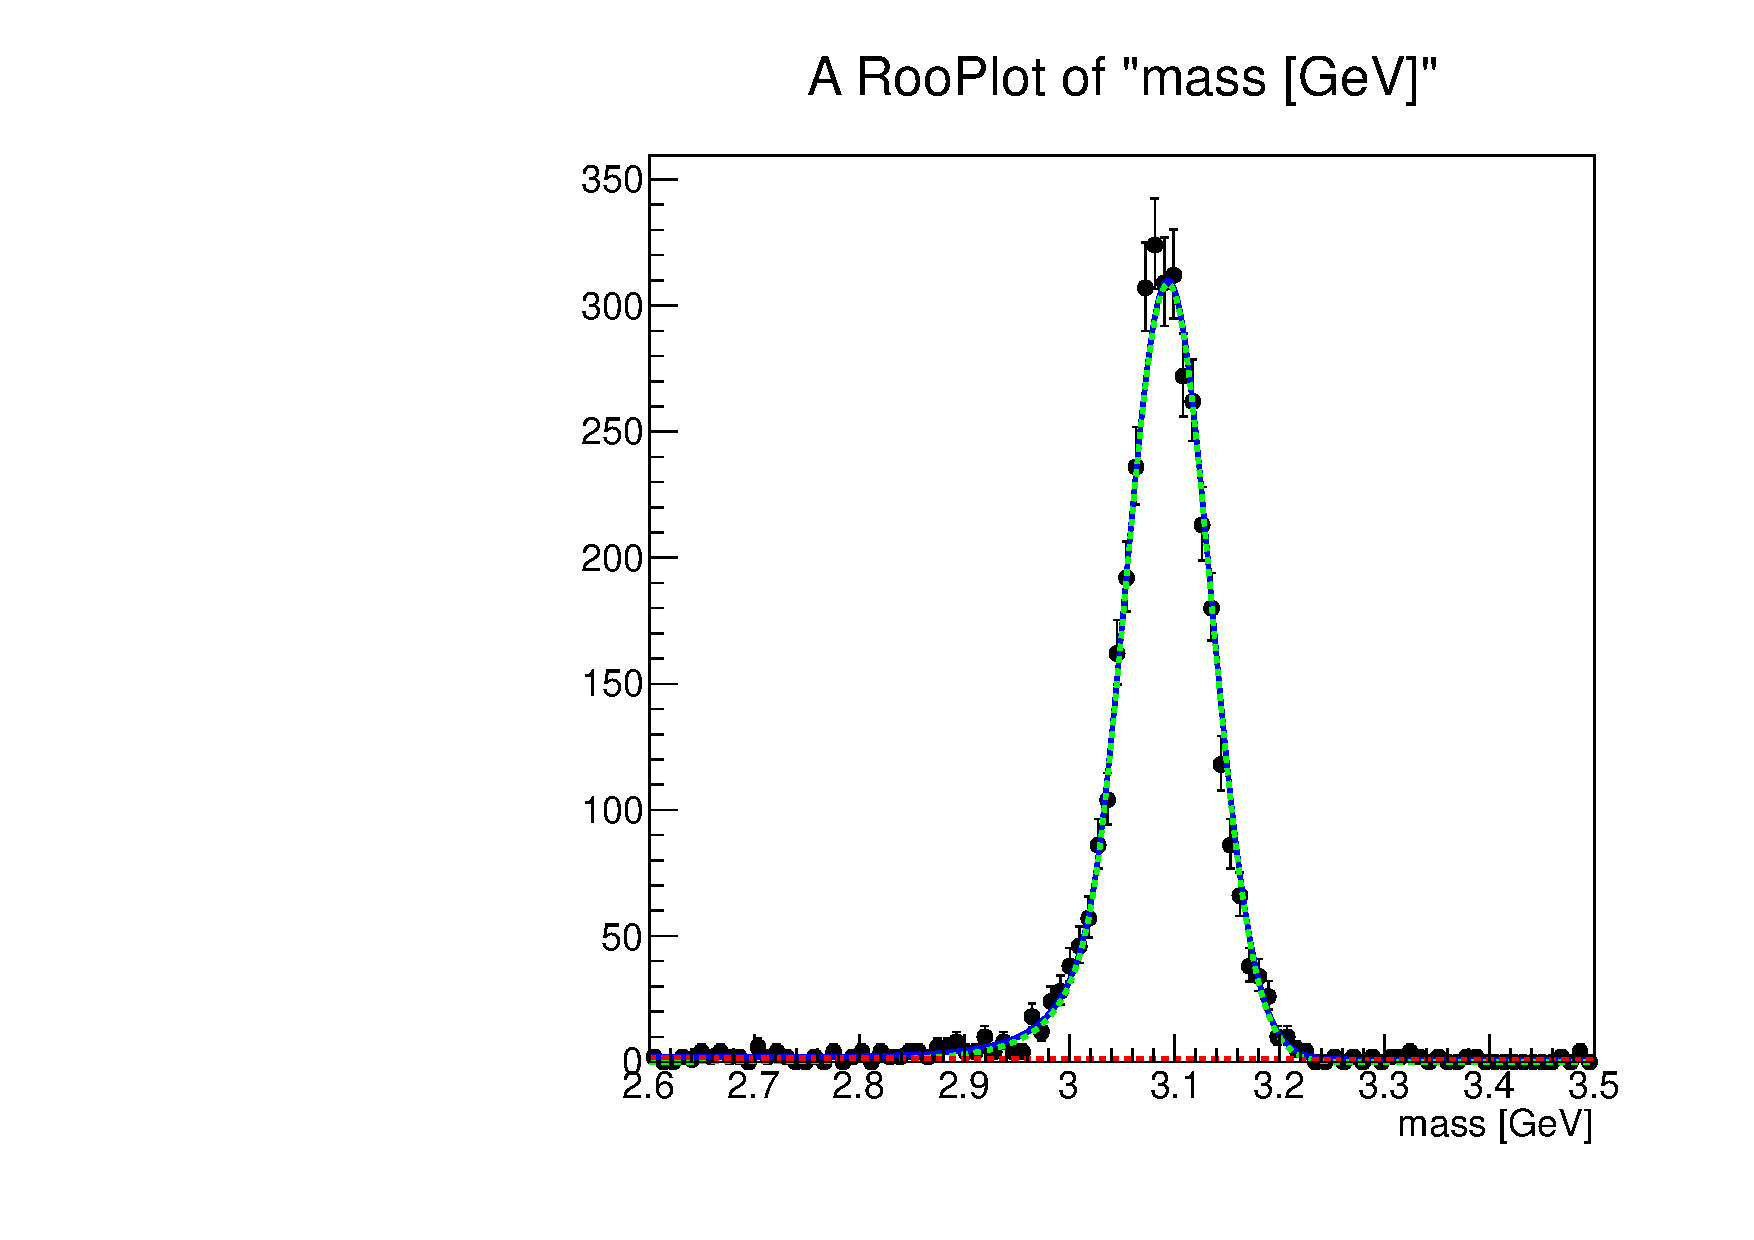
\includegraphics[width=0.25\textwidth]{../PlotsRooFitMC/croofit_trg_pass_1.pdf}
    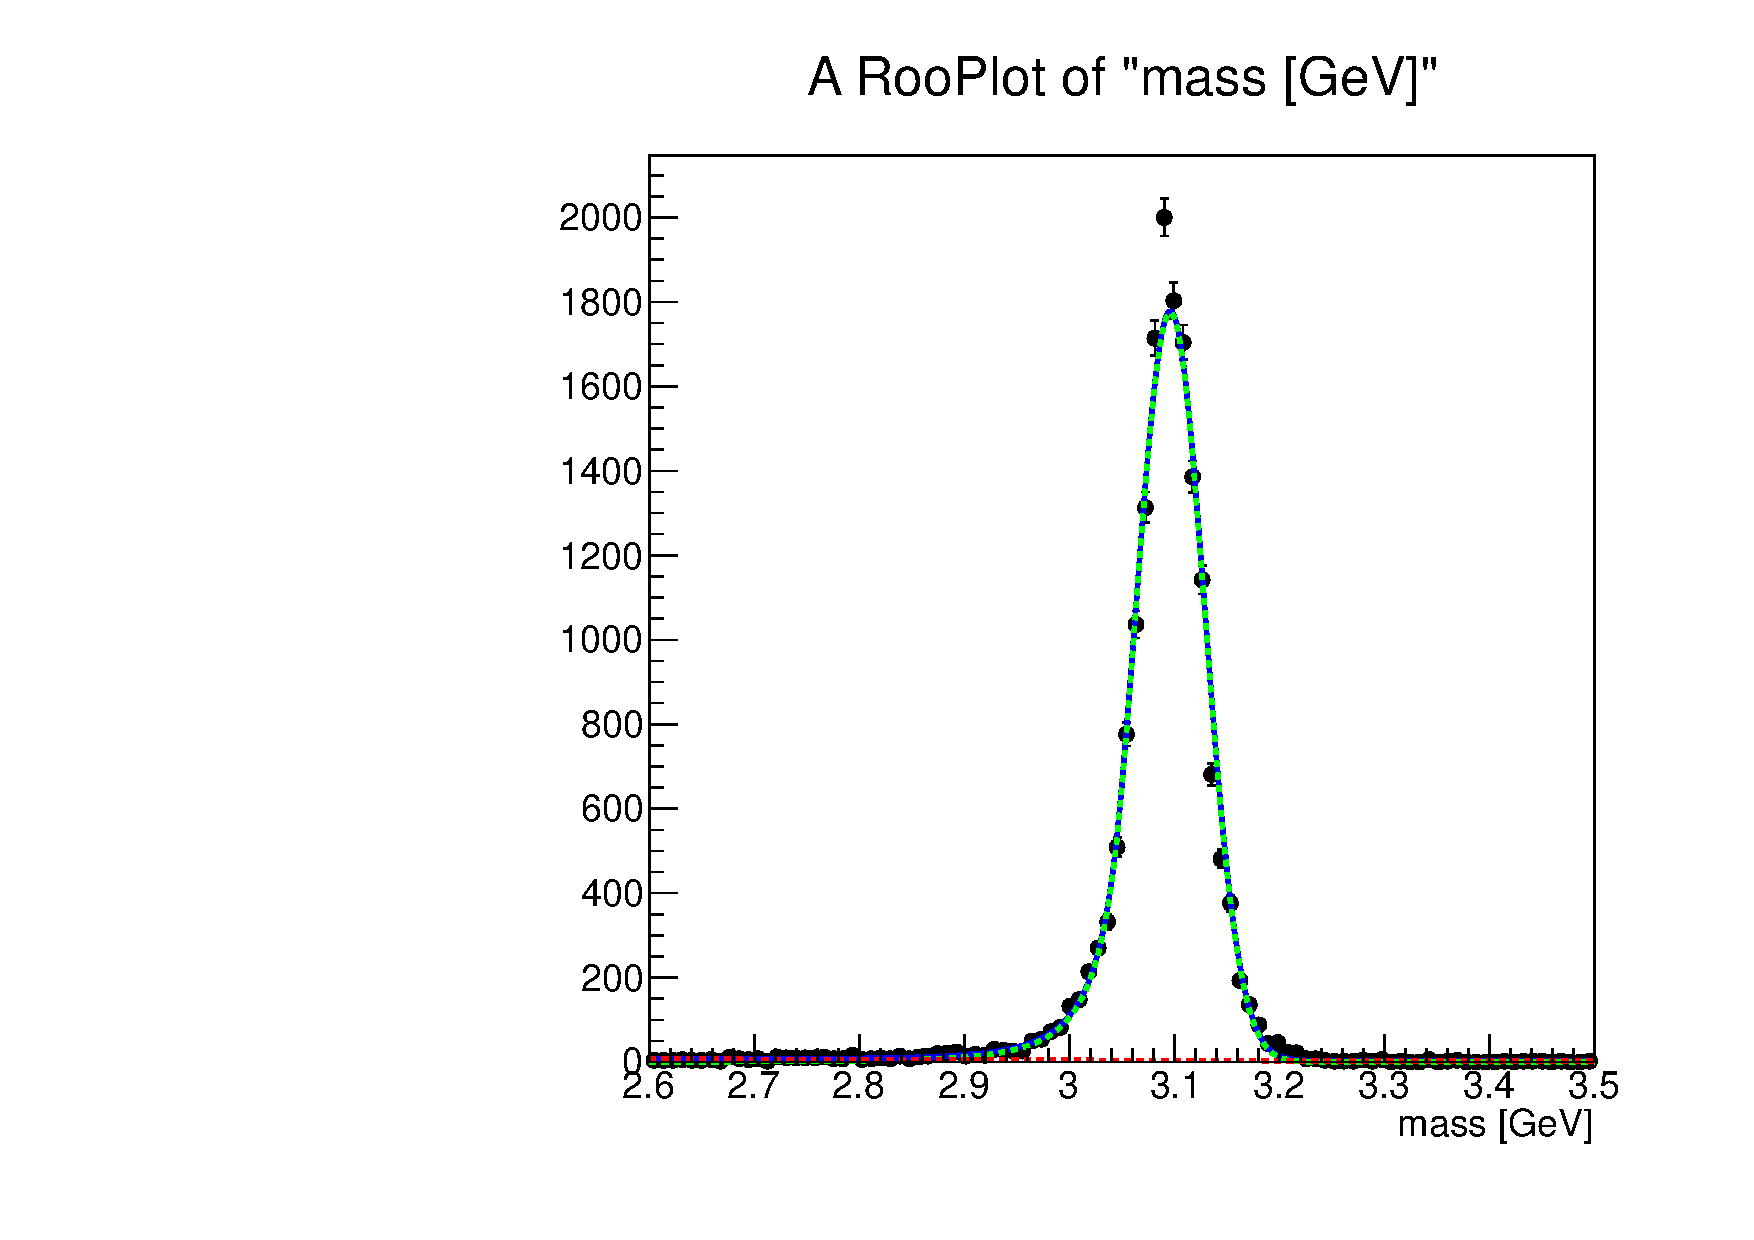
\includegraphics[width=0.25\textwidth]{../PlotsRooFitMC/croofit_trg_pass_2.pdf}
    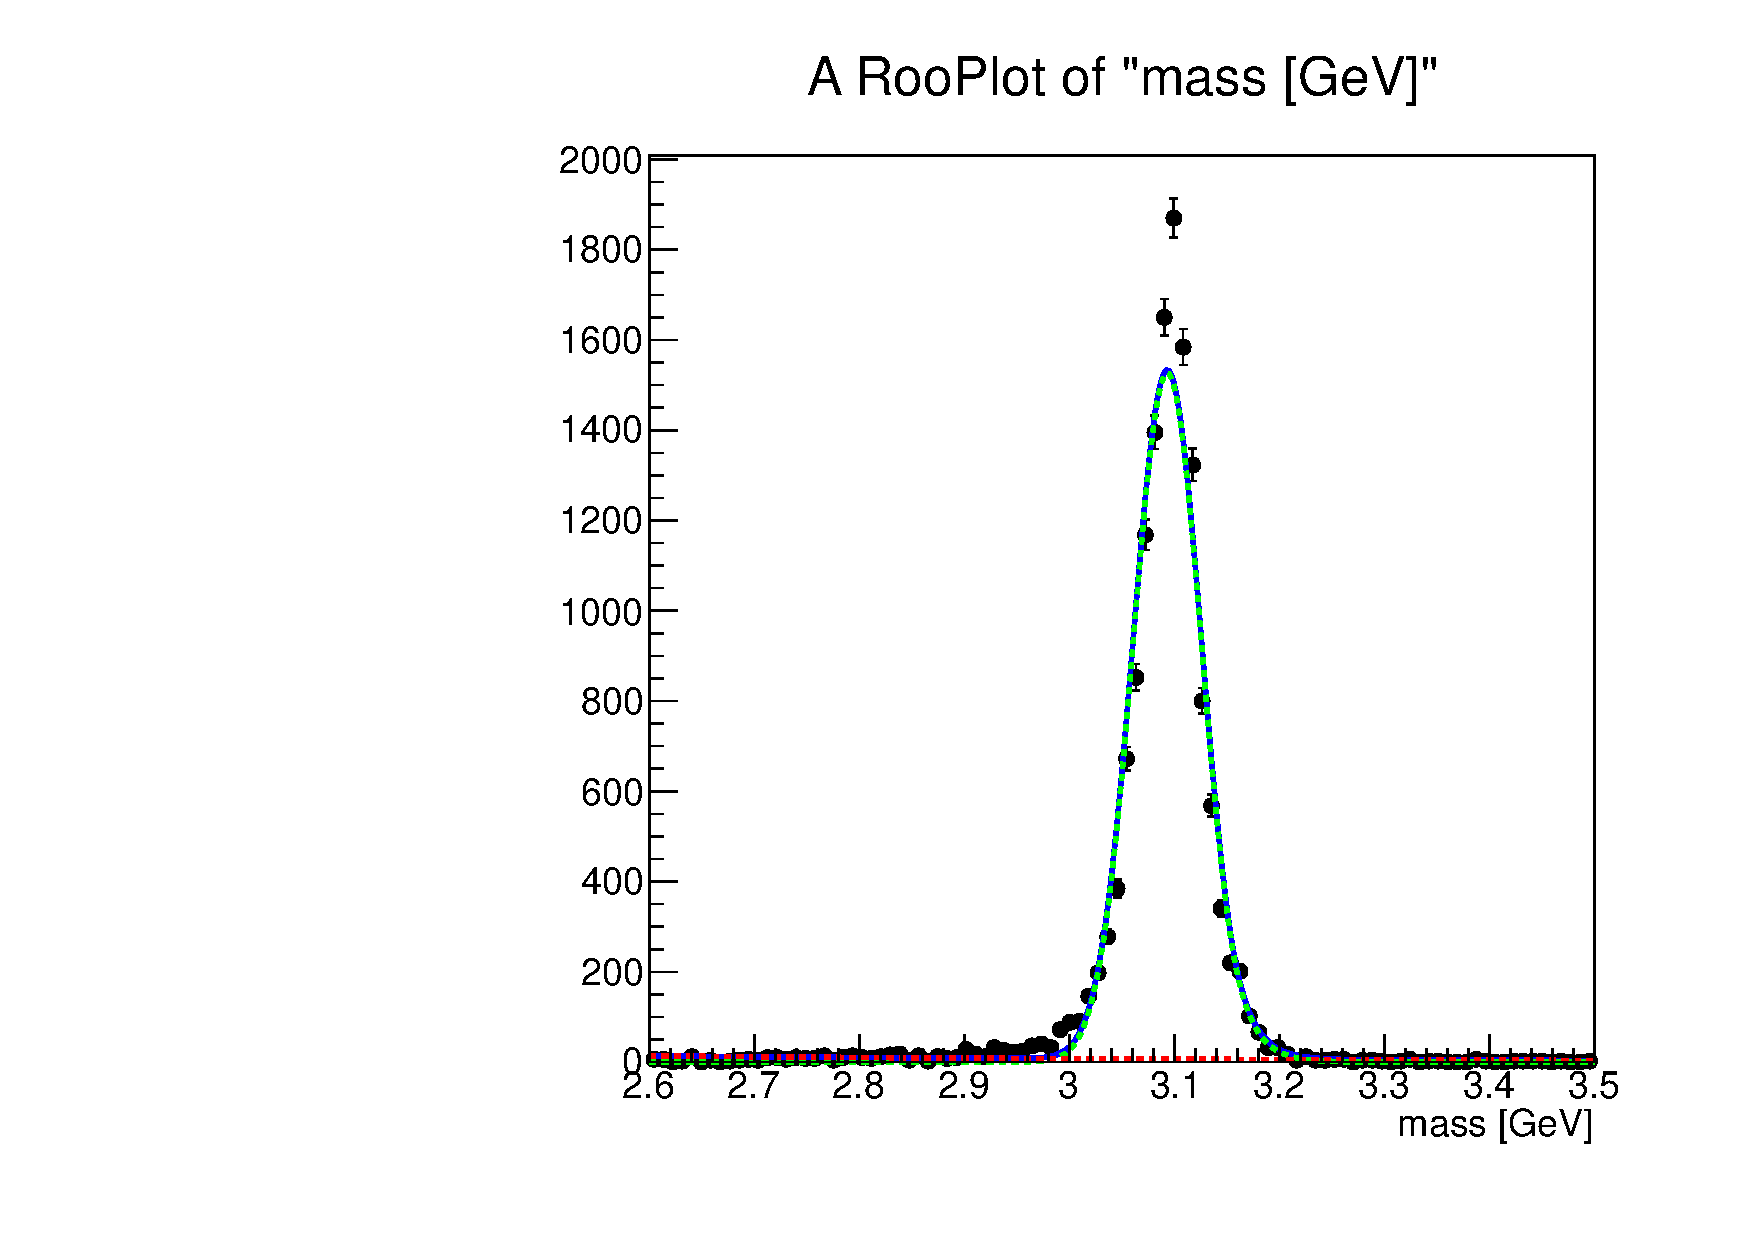
\includegraphics[width=0.25\textwidth]{../PlotsRooFitMC/croofit_trg_pass_3.pdf}
    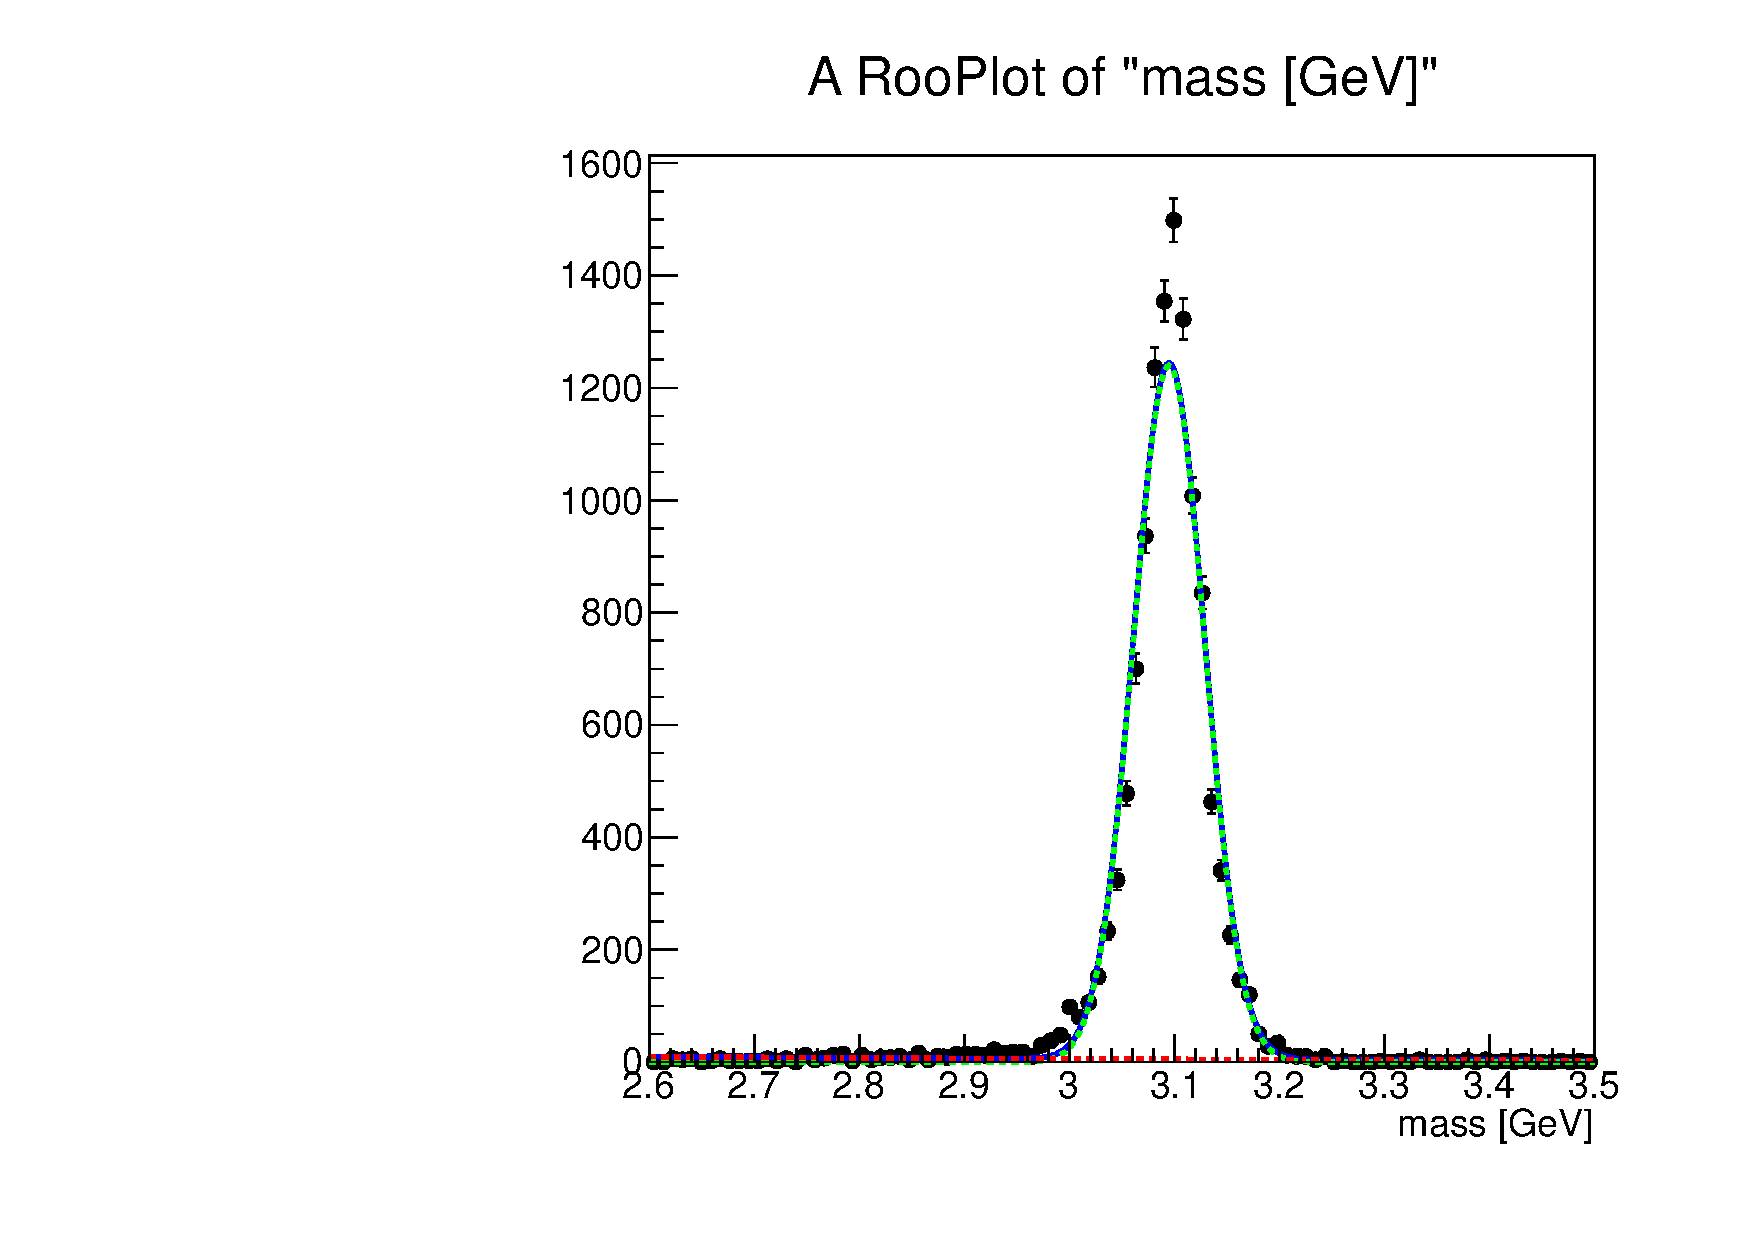
\includegraphics[width=0.25\textwidth]{../PlotsRooFitMC/croofit_trg_pass_4.pdf}
    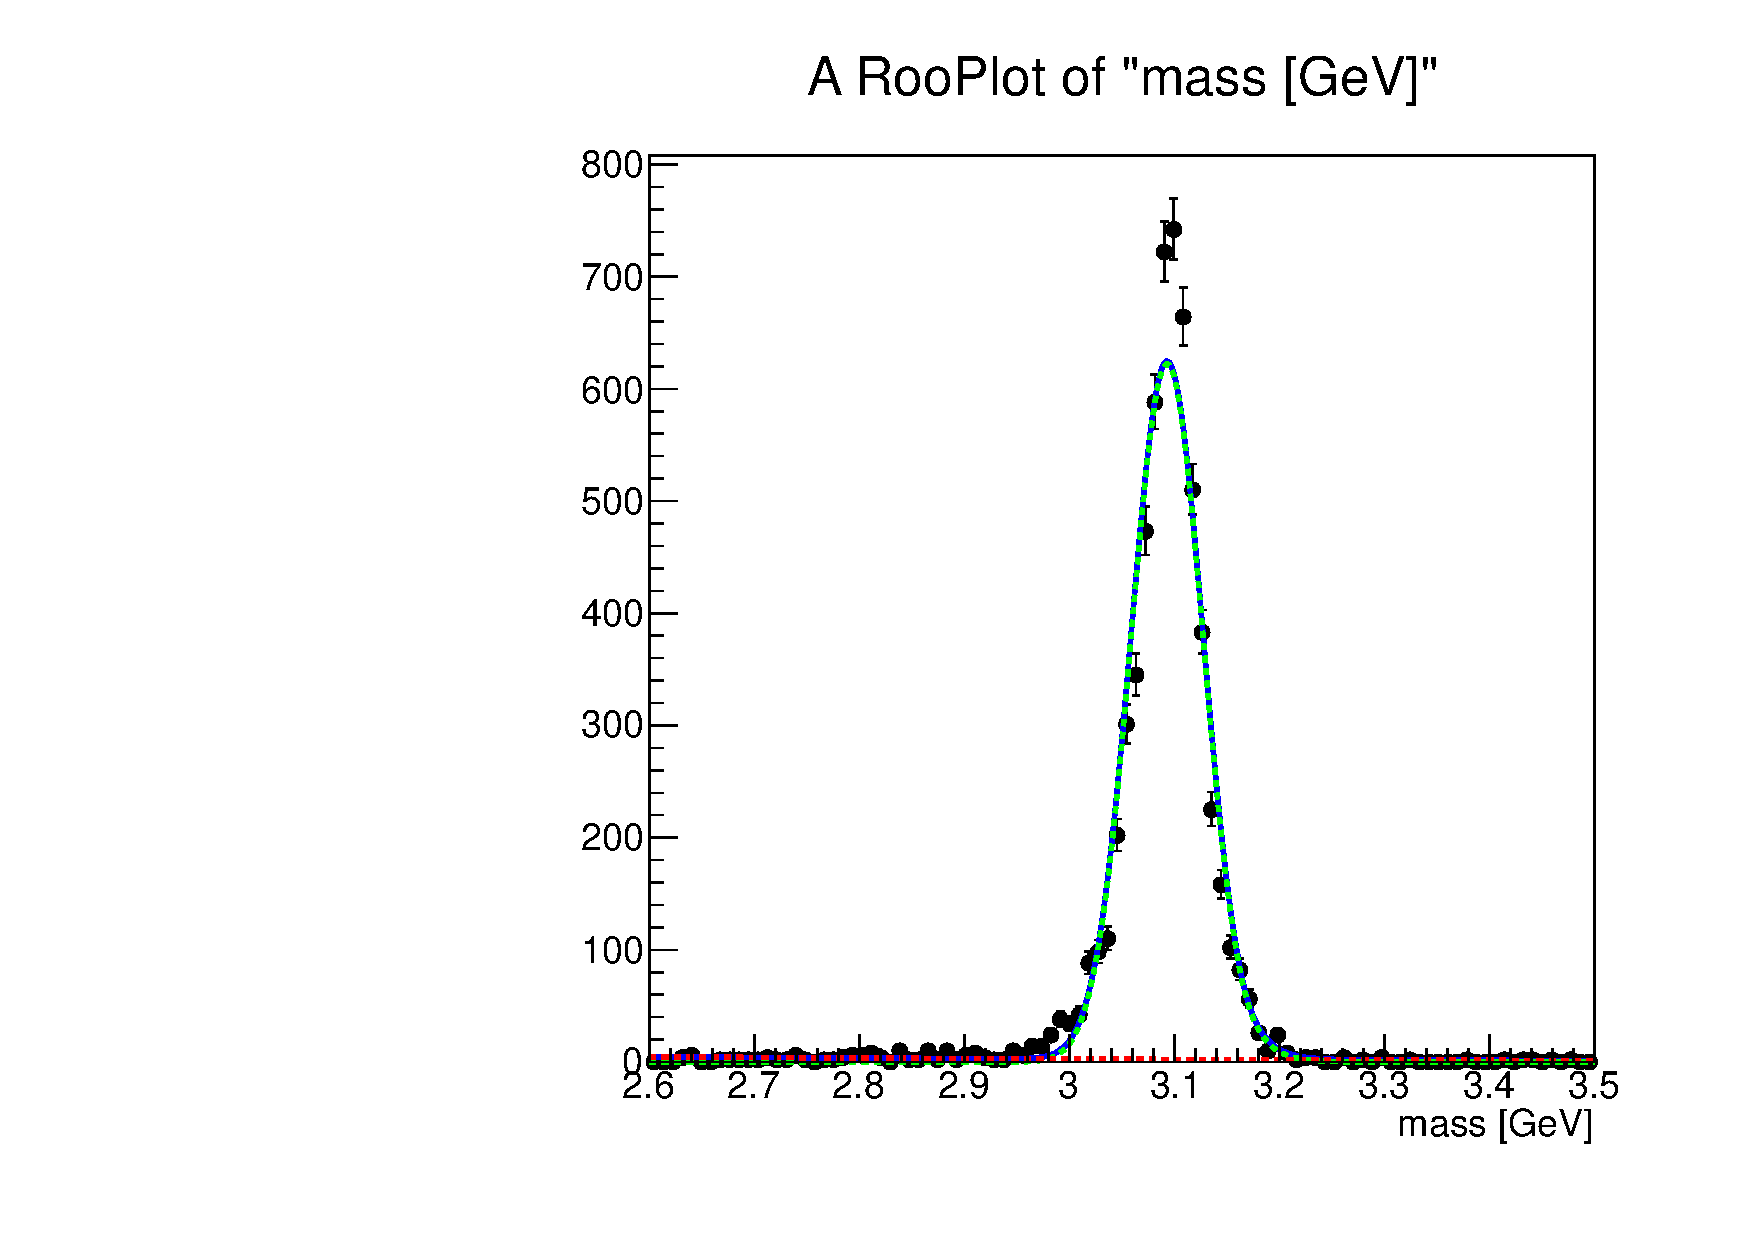
\includegraphics[width=0.25\textwidth]{../PlotsRooFitMC/croofit_trg_pass_5.pdf}
    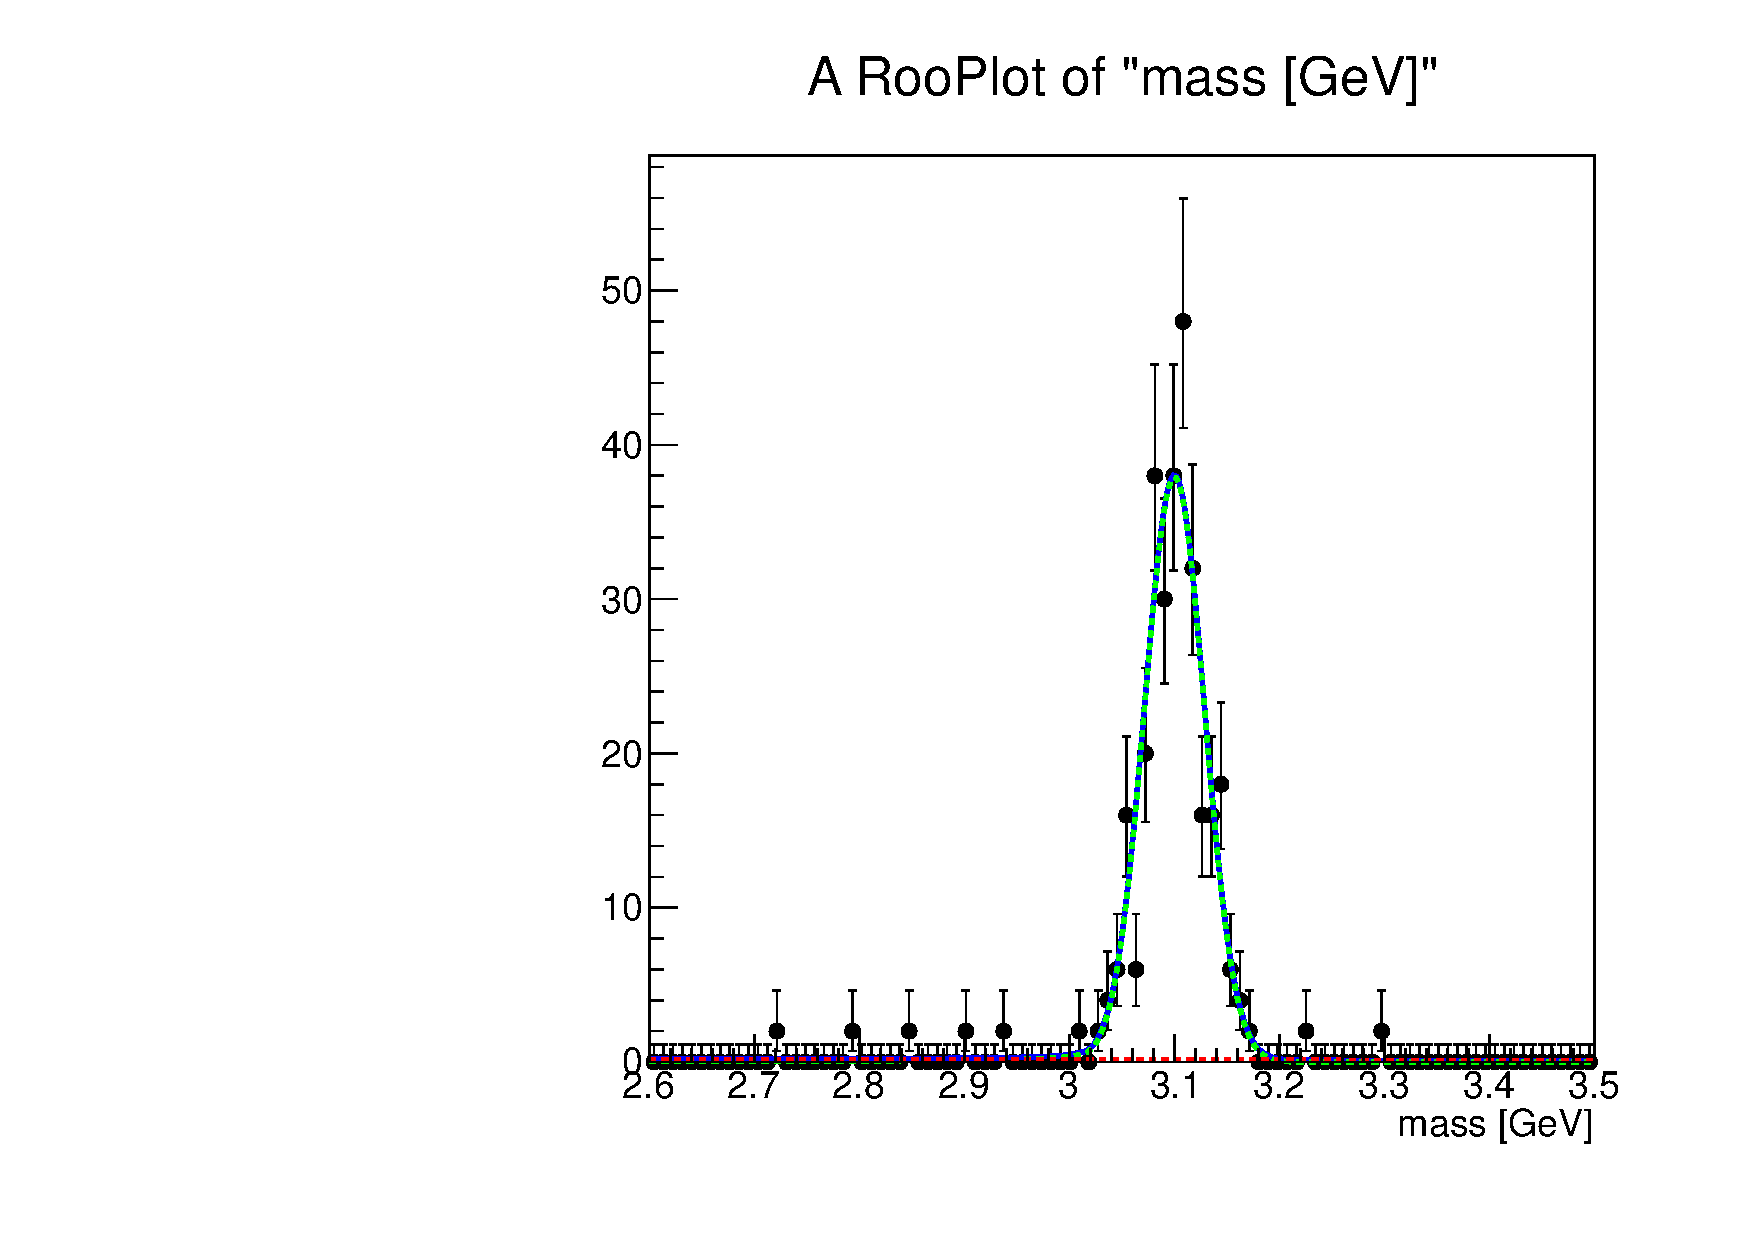
\includegraphics[width=0.25\textwidth]{../PlotsRooFitMC/croofit_trg_pass_6.pdf}
    \caption{MC Results trigger studies for passing probes, muon transverse momenta
    $\rm p_{t}$ (GeV/c)= {0.0-1.5}, {1.5-3.0}, {3.0-4.5}, {4.5-6.0}, 
    {6.0-9.0}, {9.0-20.0}, {20.0-30.0}}
   % \label{simulationfigure}
\end{figure}

\begin{figure}
    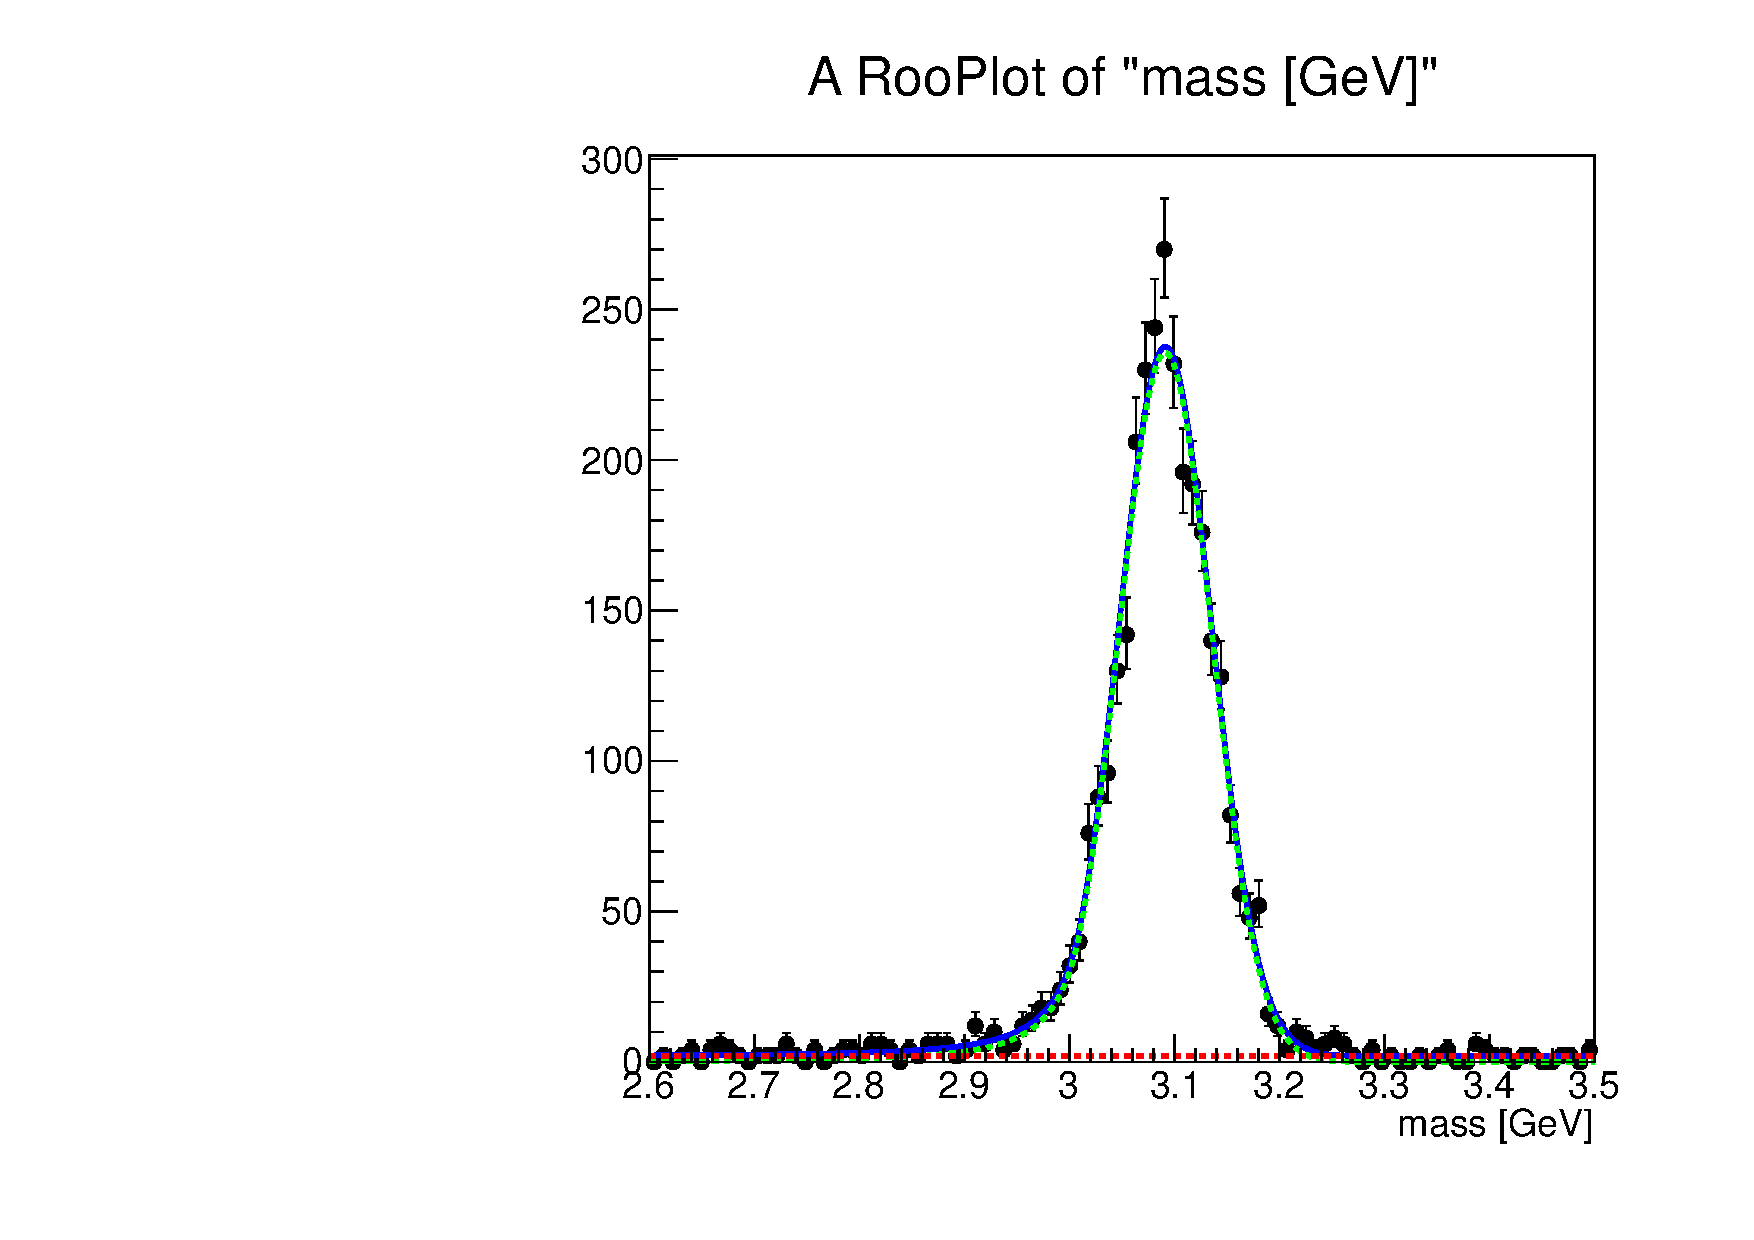
\includegraphics[width=0.25\textwidth]{../PlotsRooFitMC/croofit_trg_fail_0.pdf}
    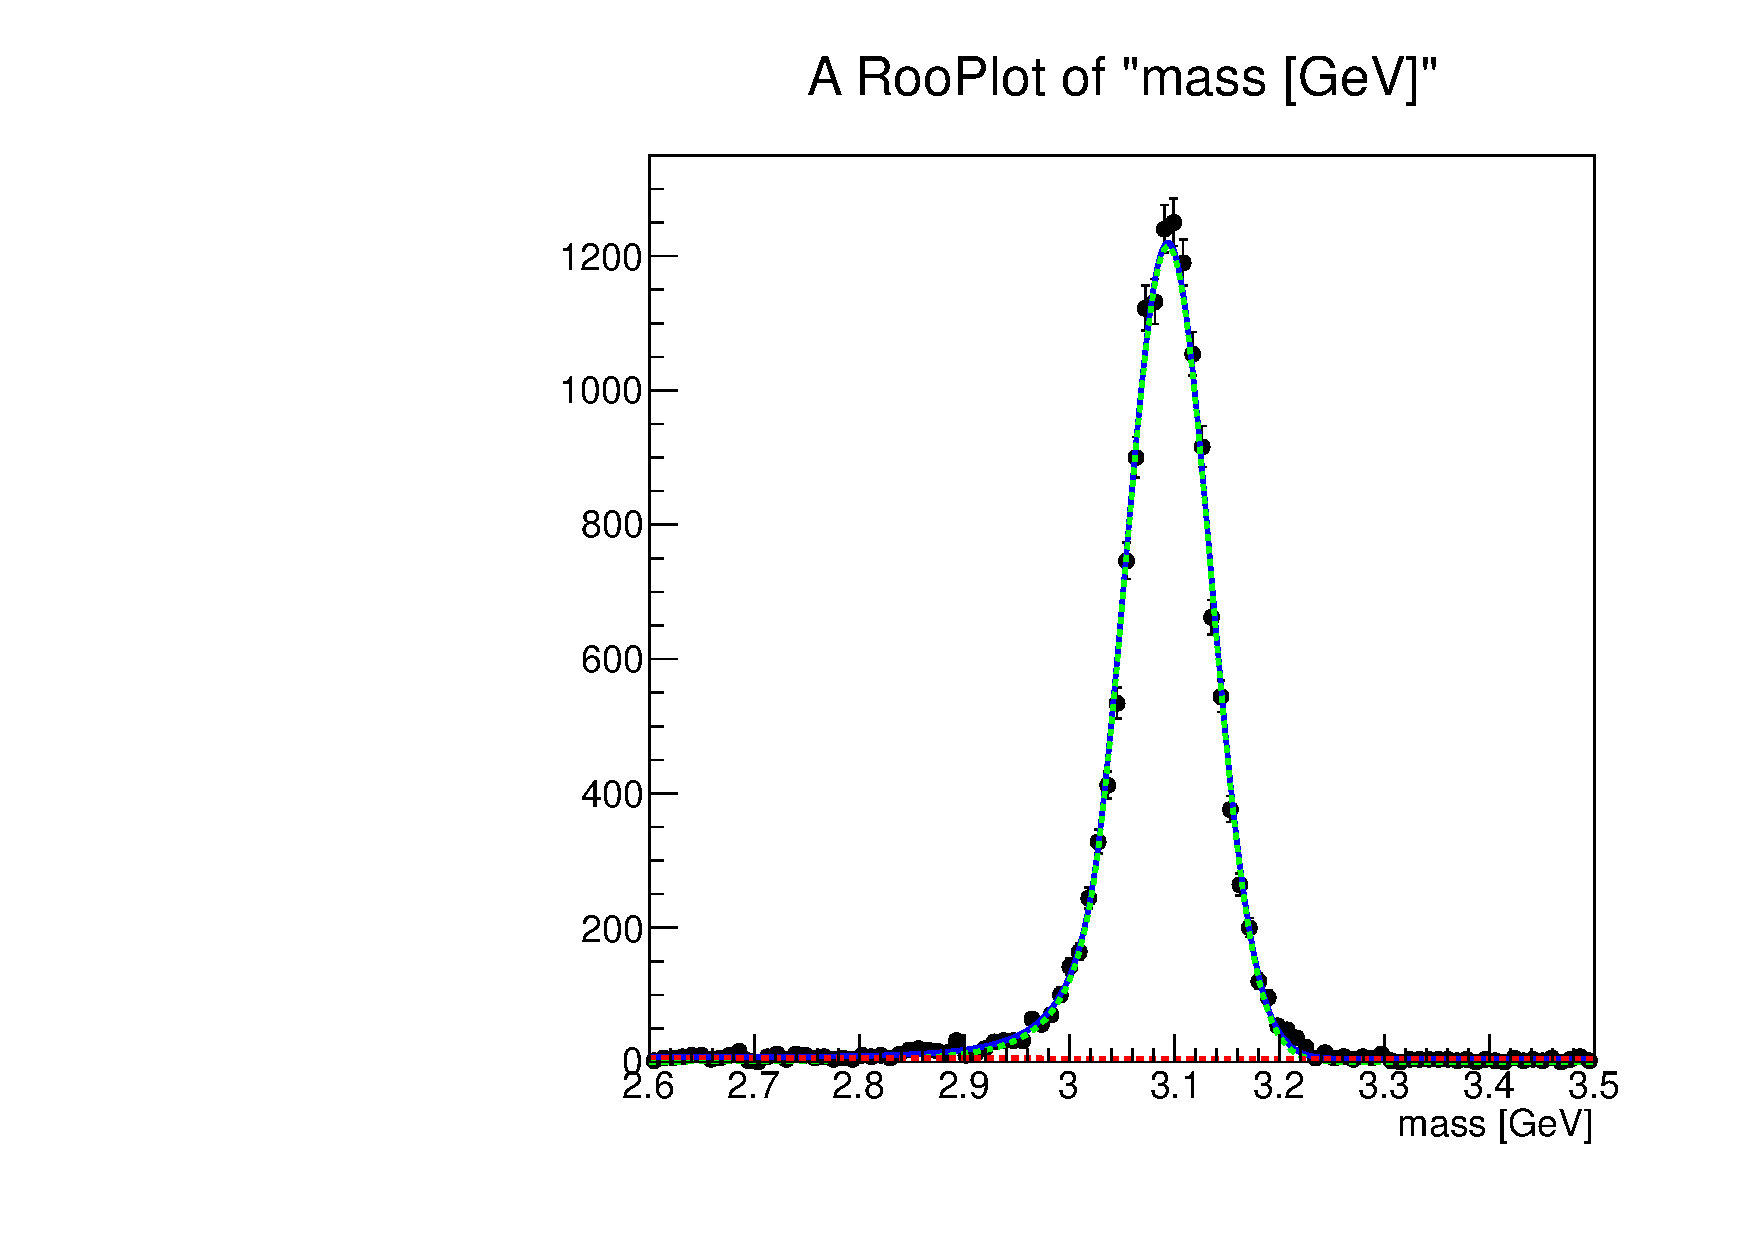
\includegraphics[width=0.25\textwidth]{../PlotsRooFitMC/croofit_trg_fail_1.pdf}
    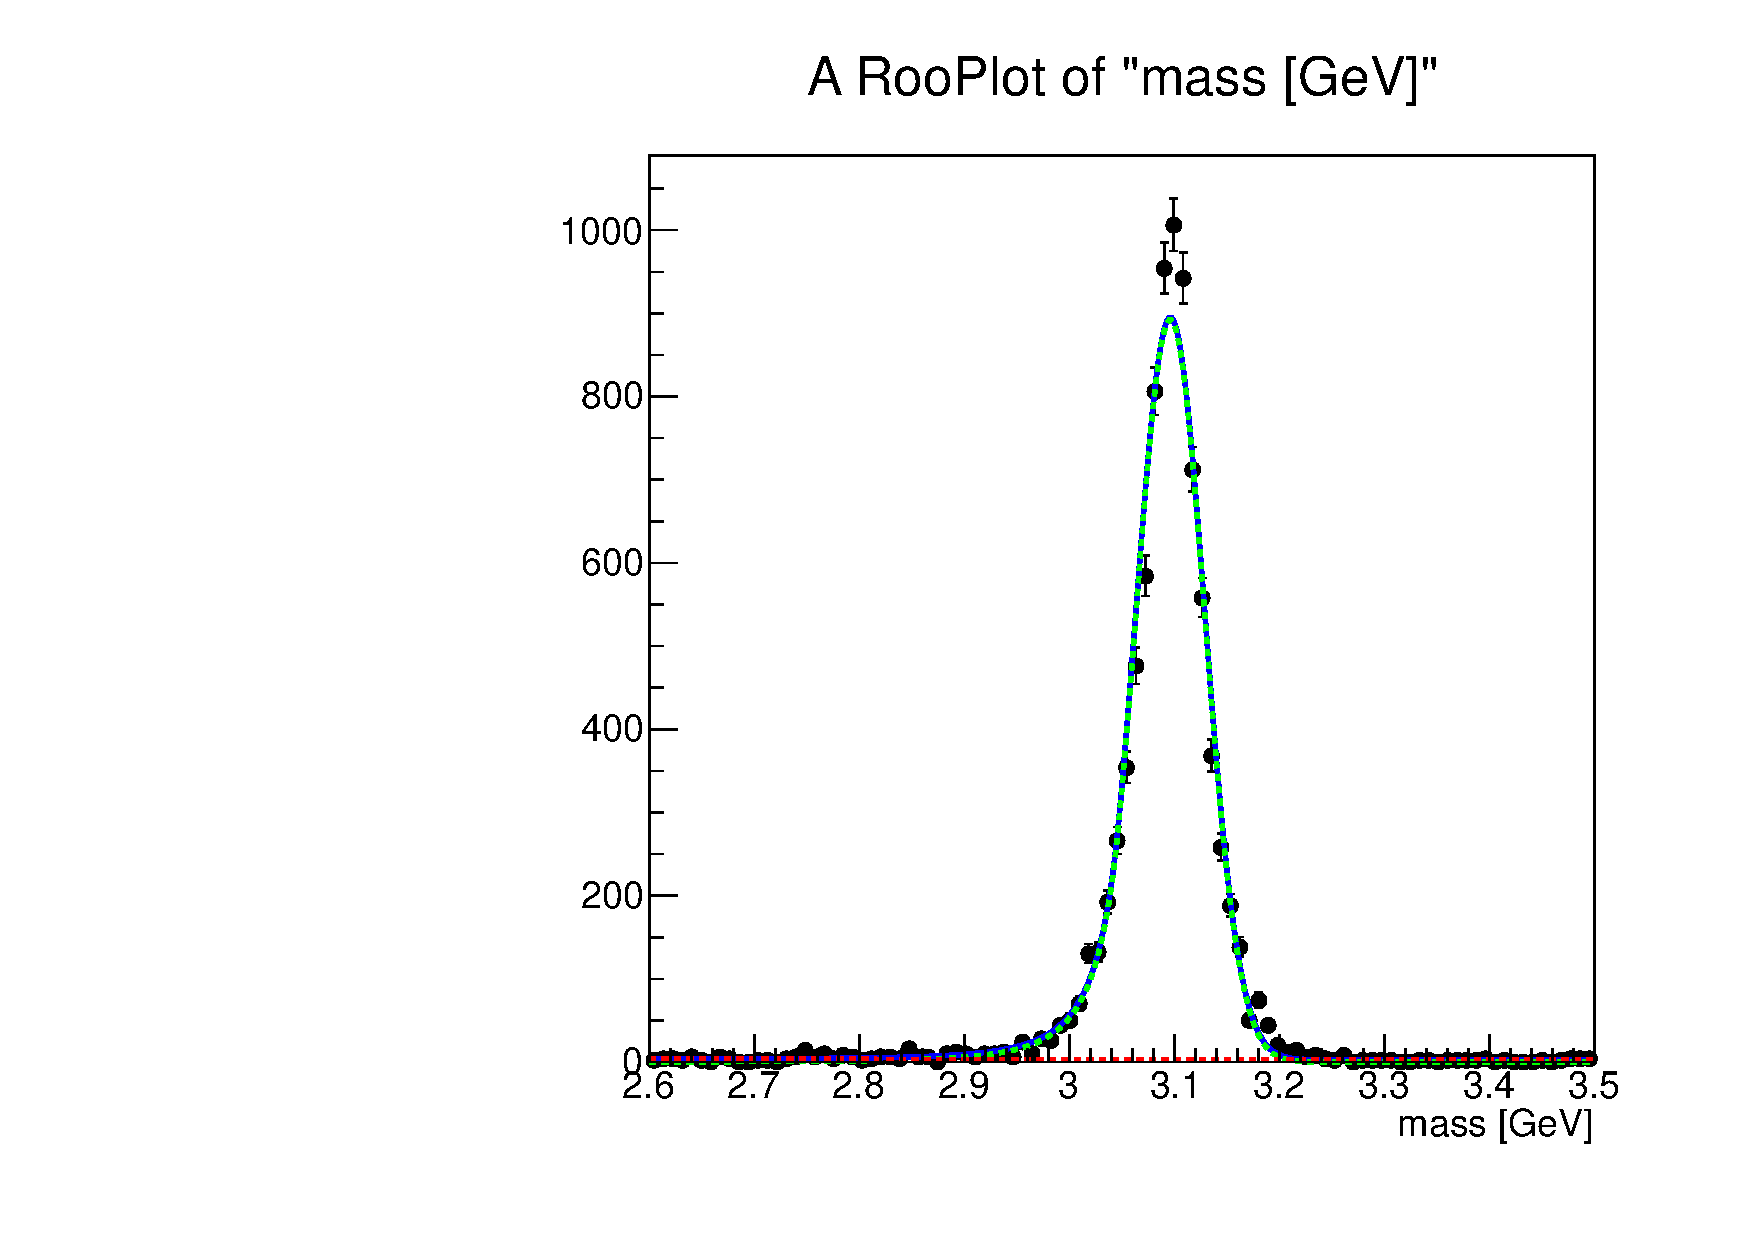
\includegraphics[width=0.25\textwidth]{../PlotsRooFitMC/croofit_trg_fail_2.pdf}
    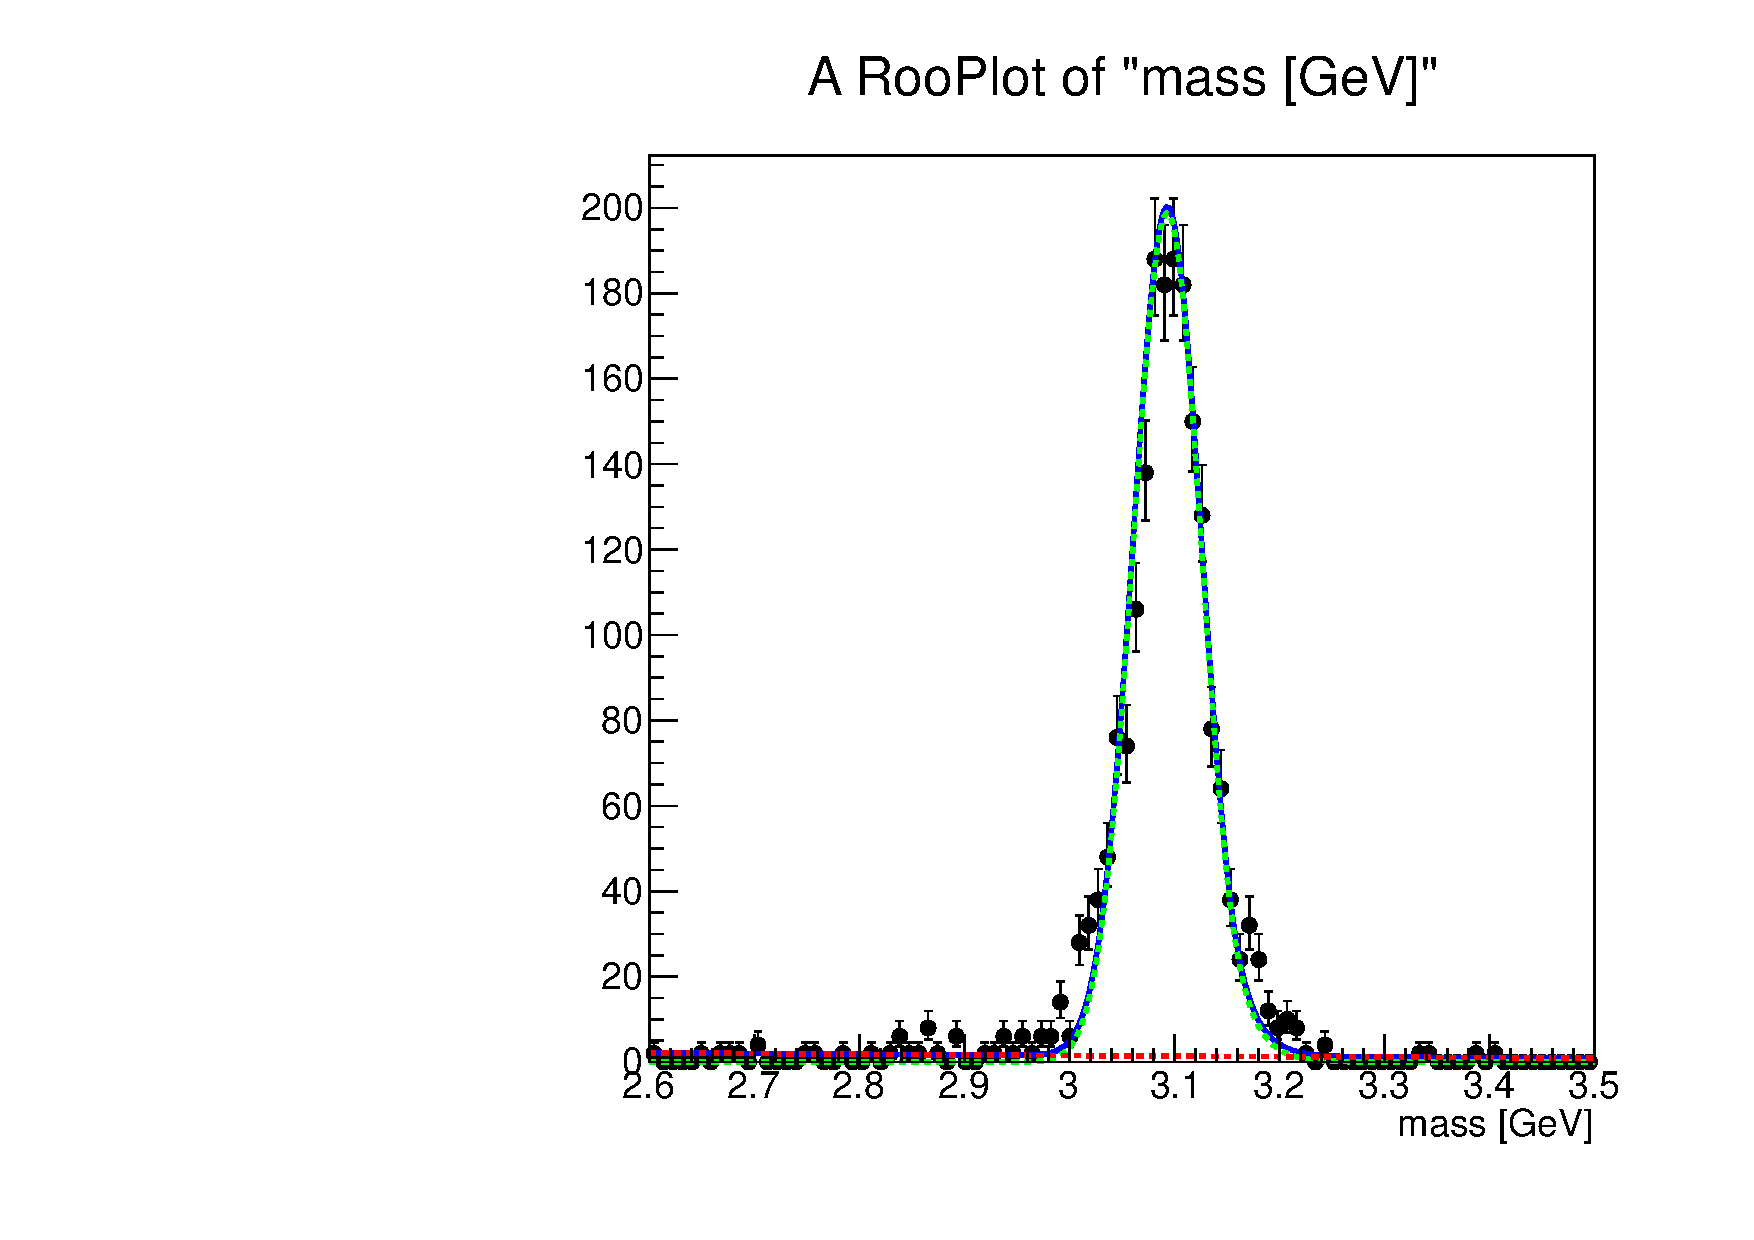
\includegraphics[width=0.25\textwidth]{../PlotsRooFitMC/croofit_trg_fail_3.pdf}
    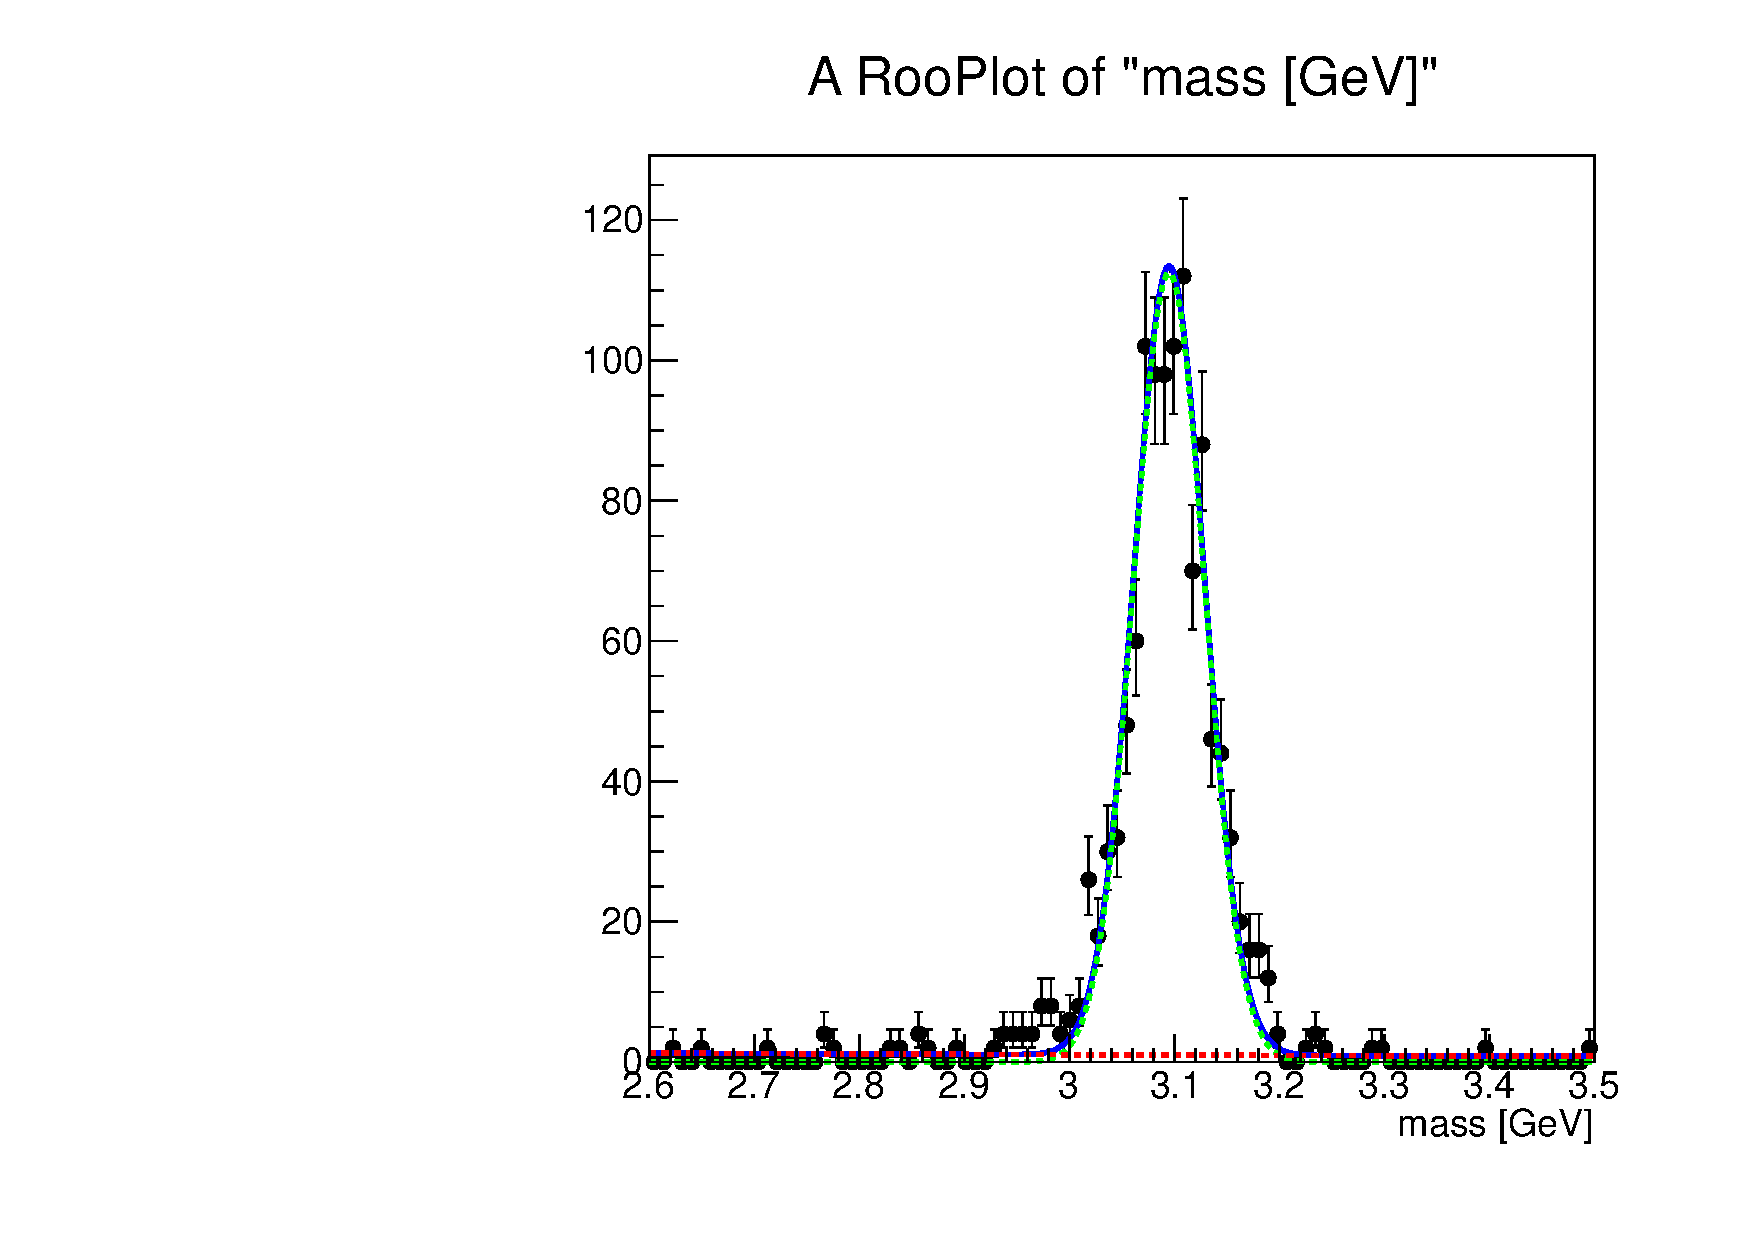
\includegraphics[width=0.25\textwidth]{../PlotsRooFitMC/croofit_trg_fail_4.pdf}
    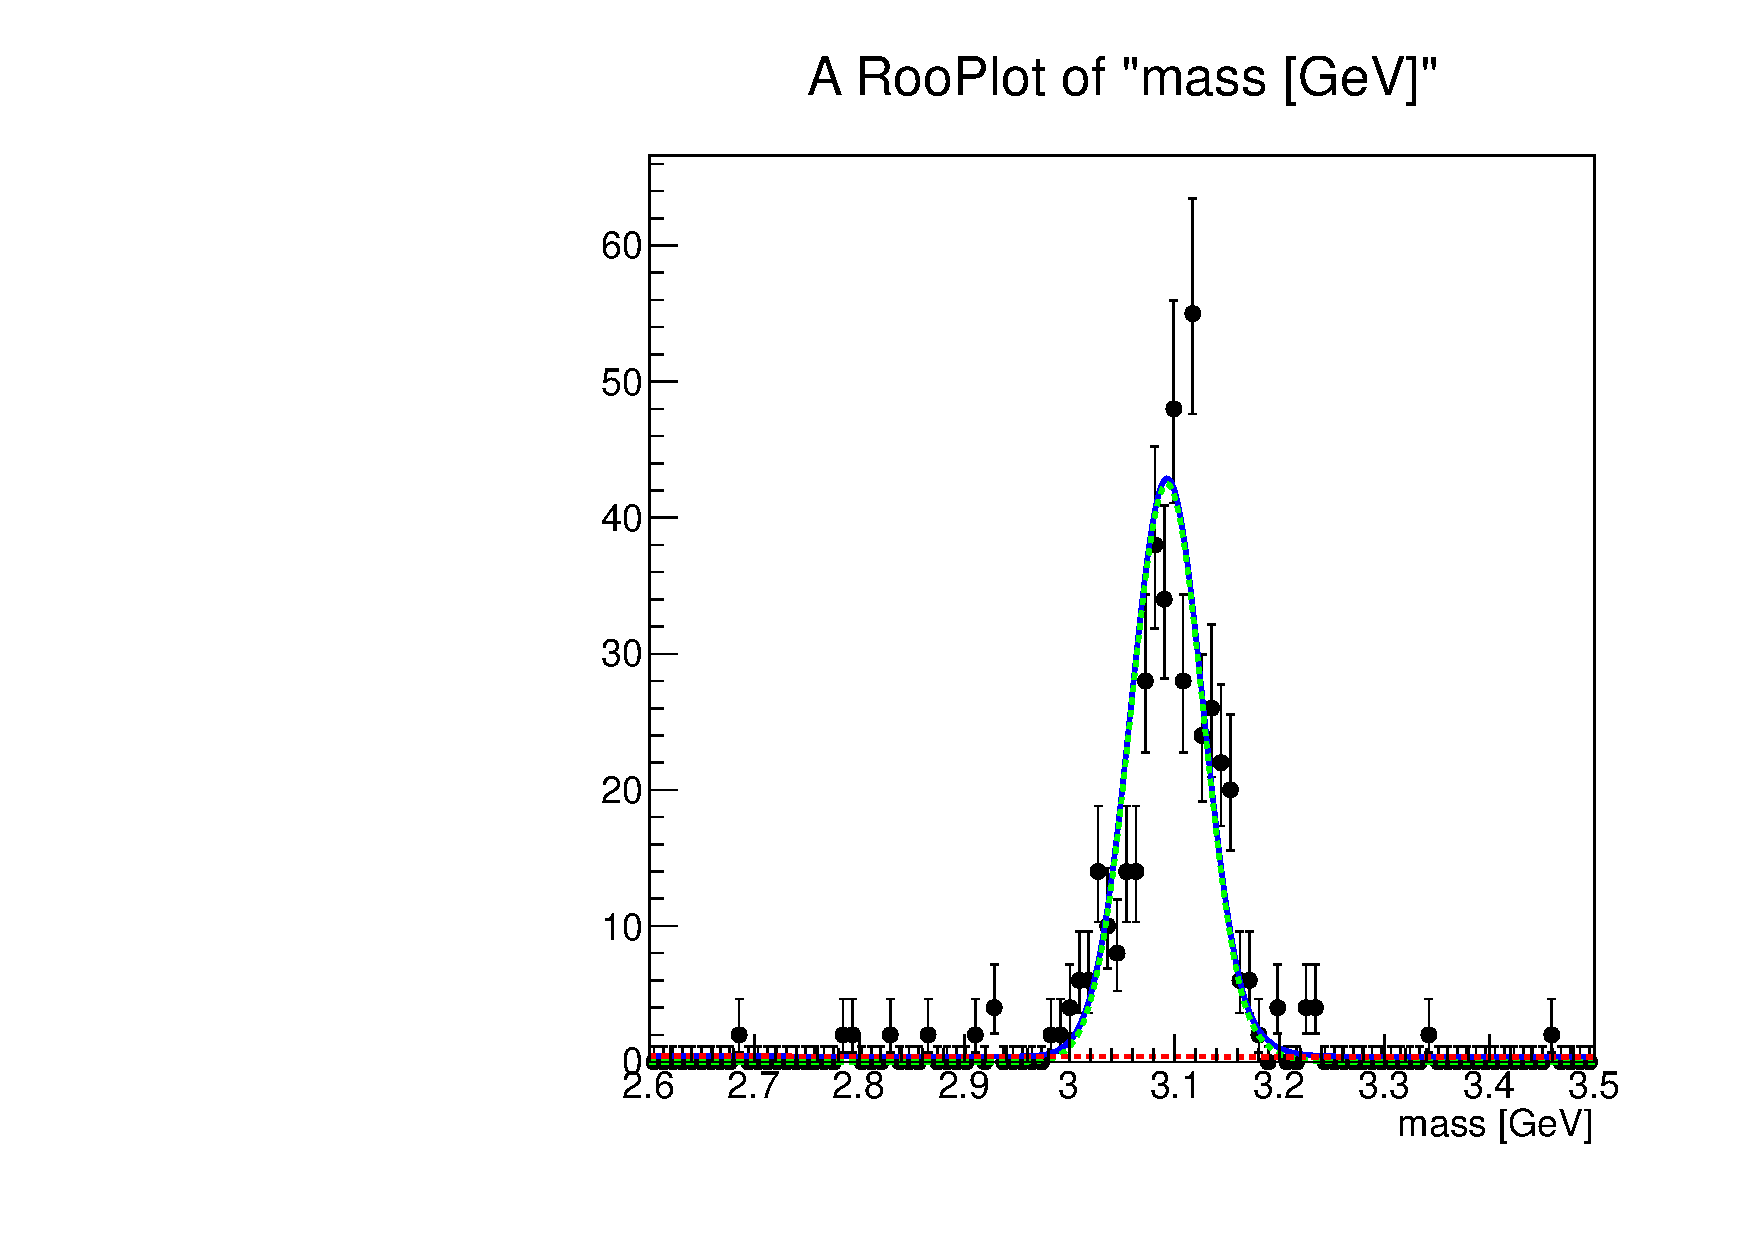
\includegraphics[width=0.25\textwidth]{../PlotsRooFitMC/croofit_trg_fail_5.pdf}
    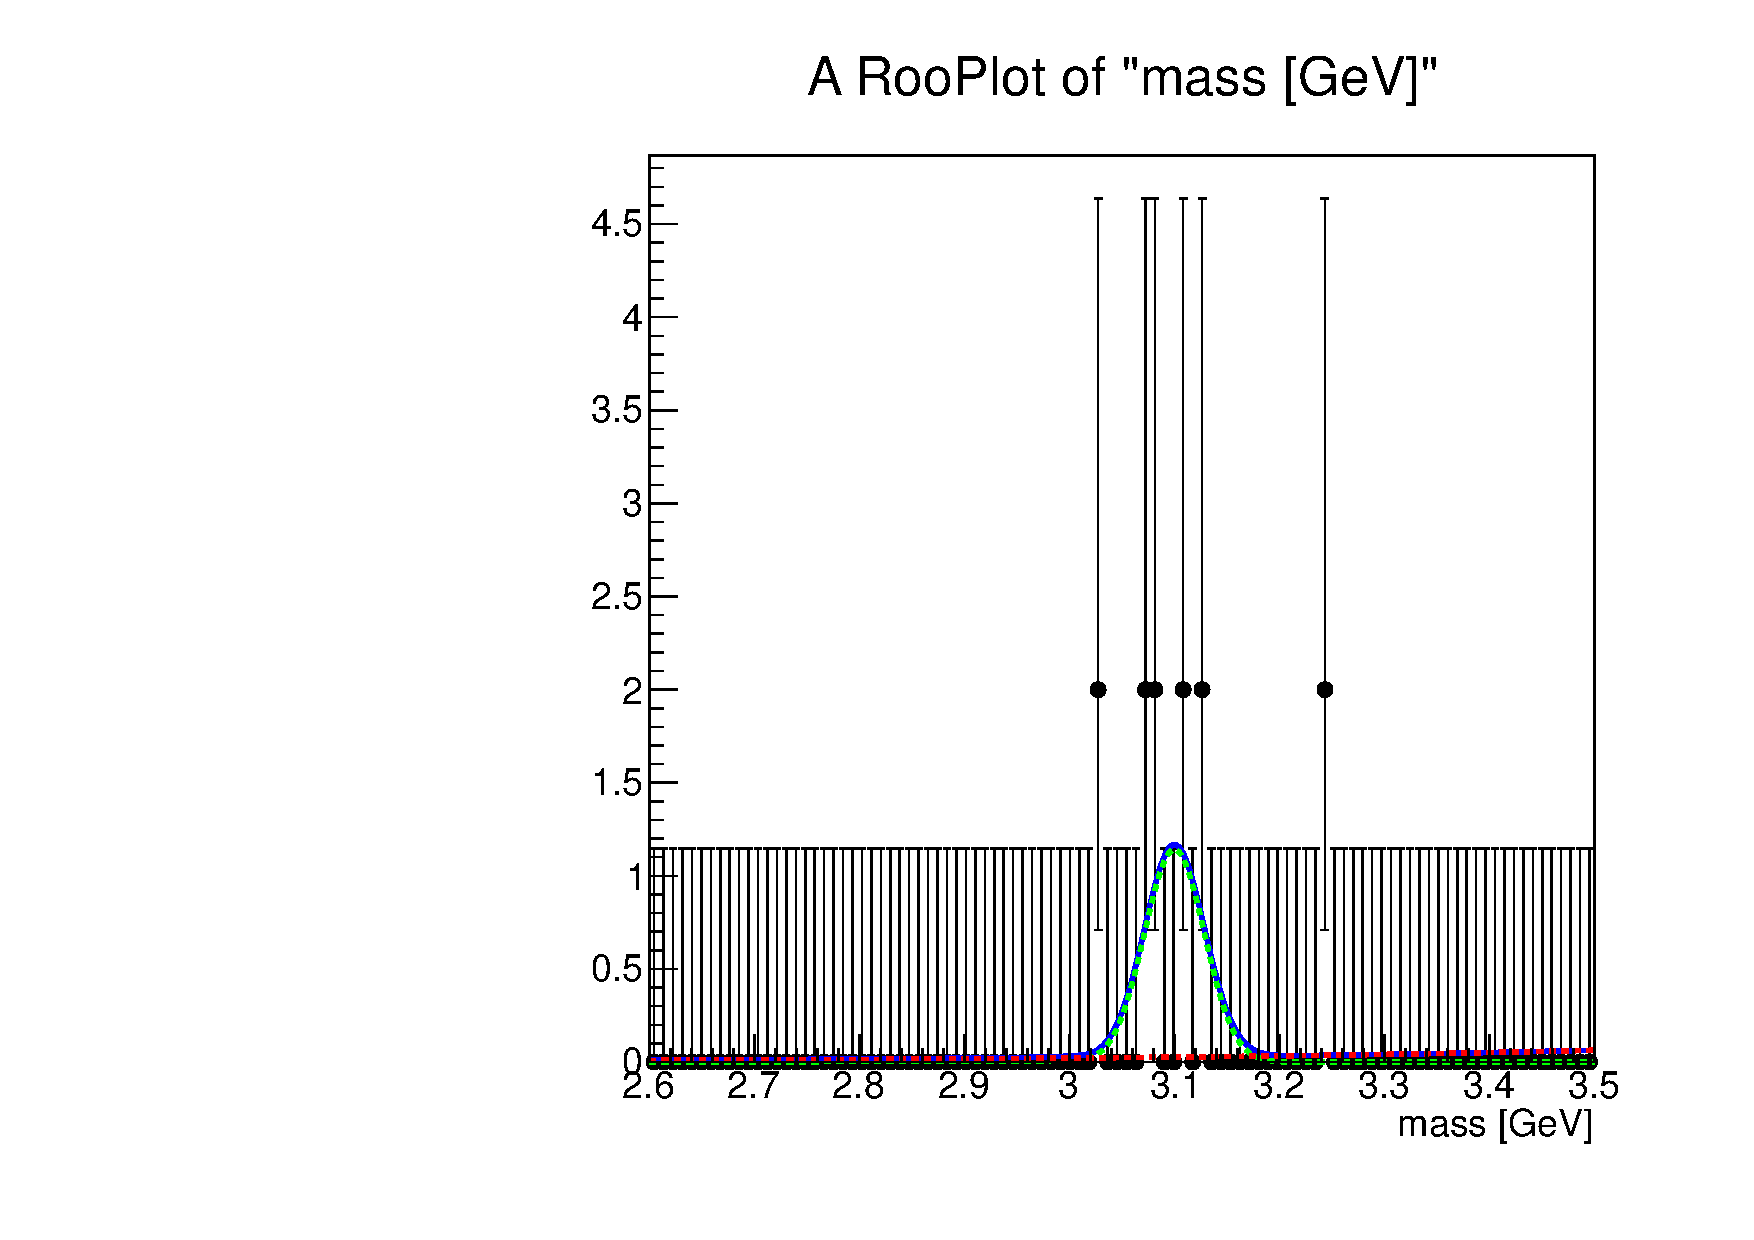
\includegraphics[width=0.25\textwidth]{../PlotsRooFitMC/croofit_trg_fail_6.pdf}
    \caption{MC Results trigger studies for failing probes, muon transverse momenta
    $\rm p_{t}$ (GeV/c)= {0.0-1.5}, {1.5-3.0}, {3.0-4.5}, {4.5-6.0}, 
    {6.0-9.0}, {9.0-20.0}, {20.0-30.0}}
   % \label{simulationfigure}
\end{figure}


\begin{figure}
    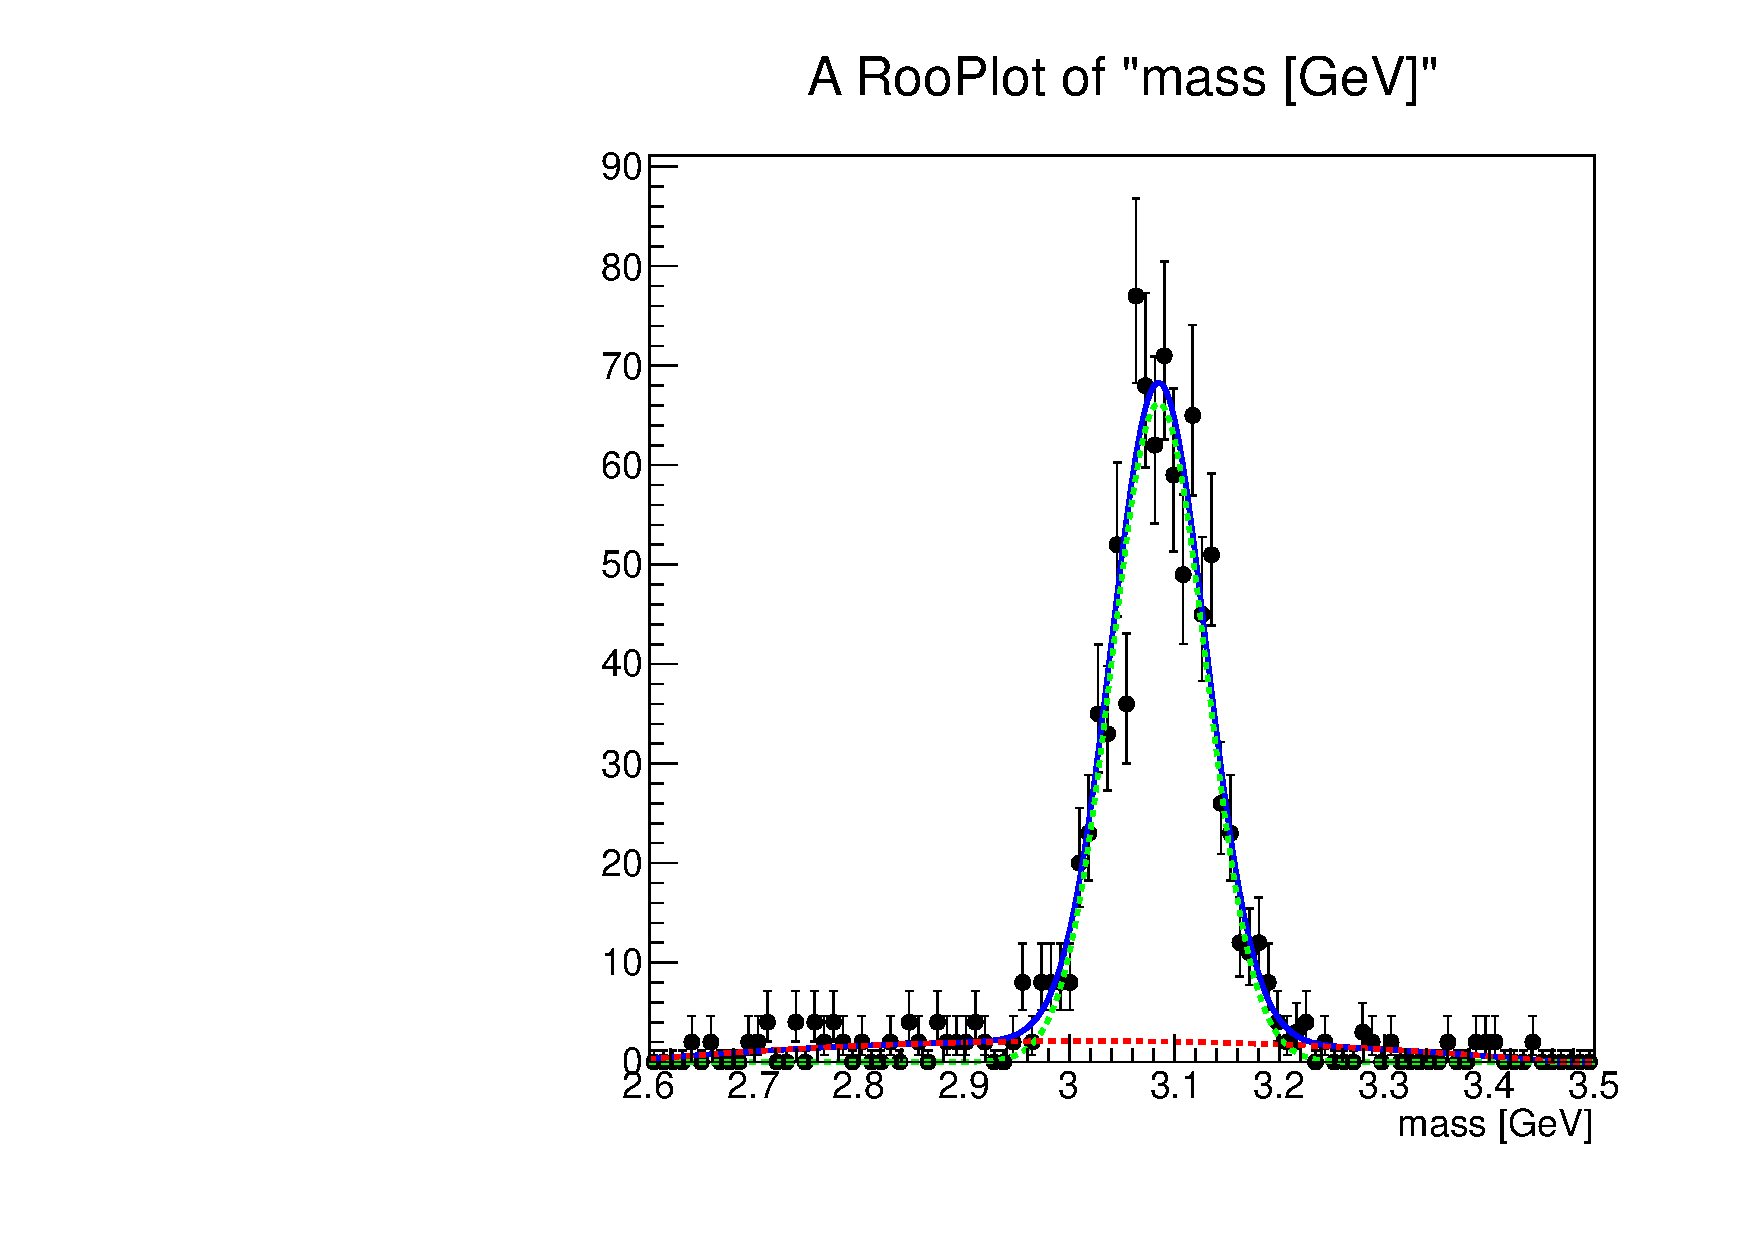
\includegraphics[width=0.25\textwidth]{../PlotsRooFitMC/croofit_trk_pass_0.pdf}
    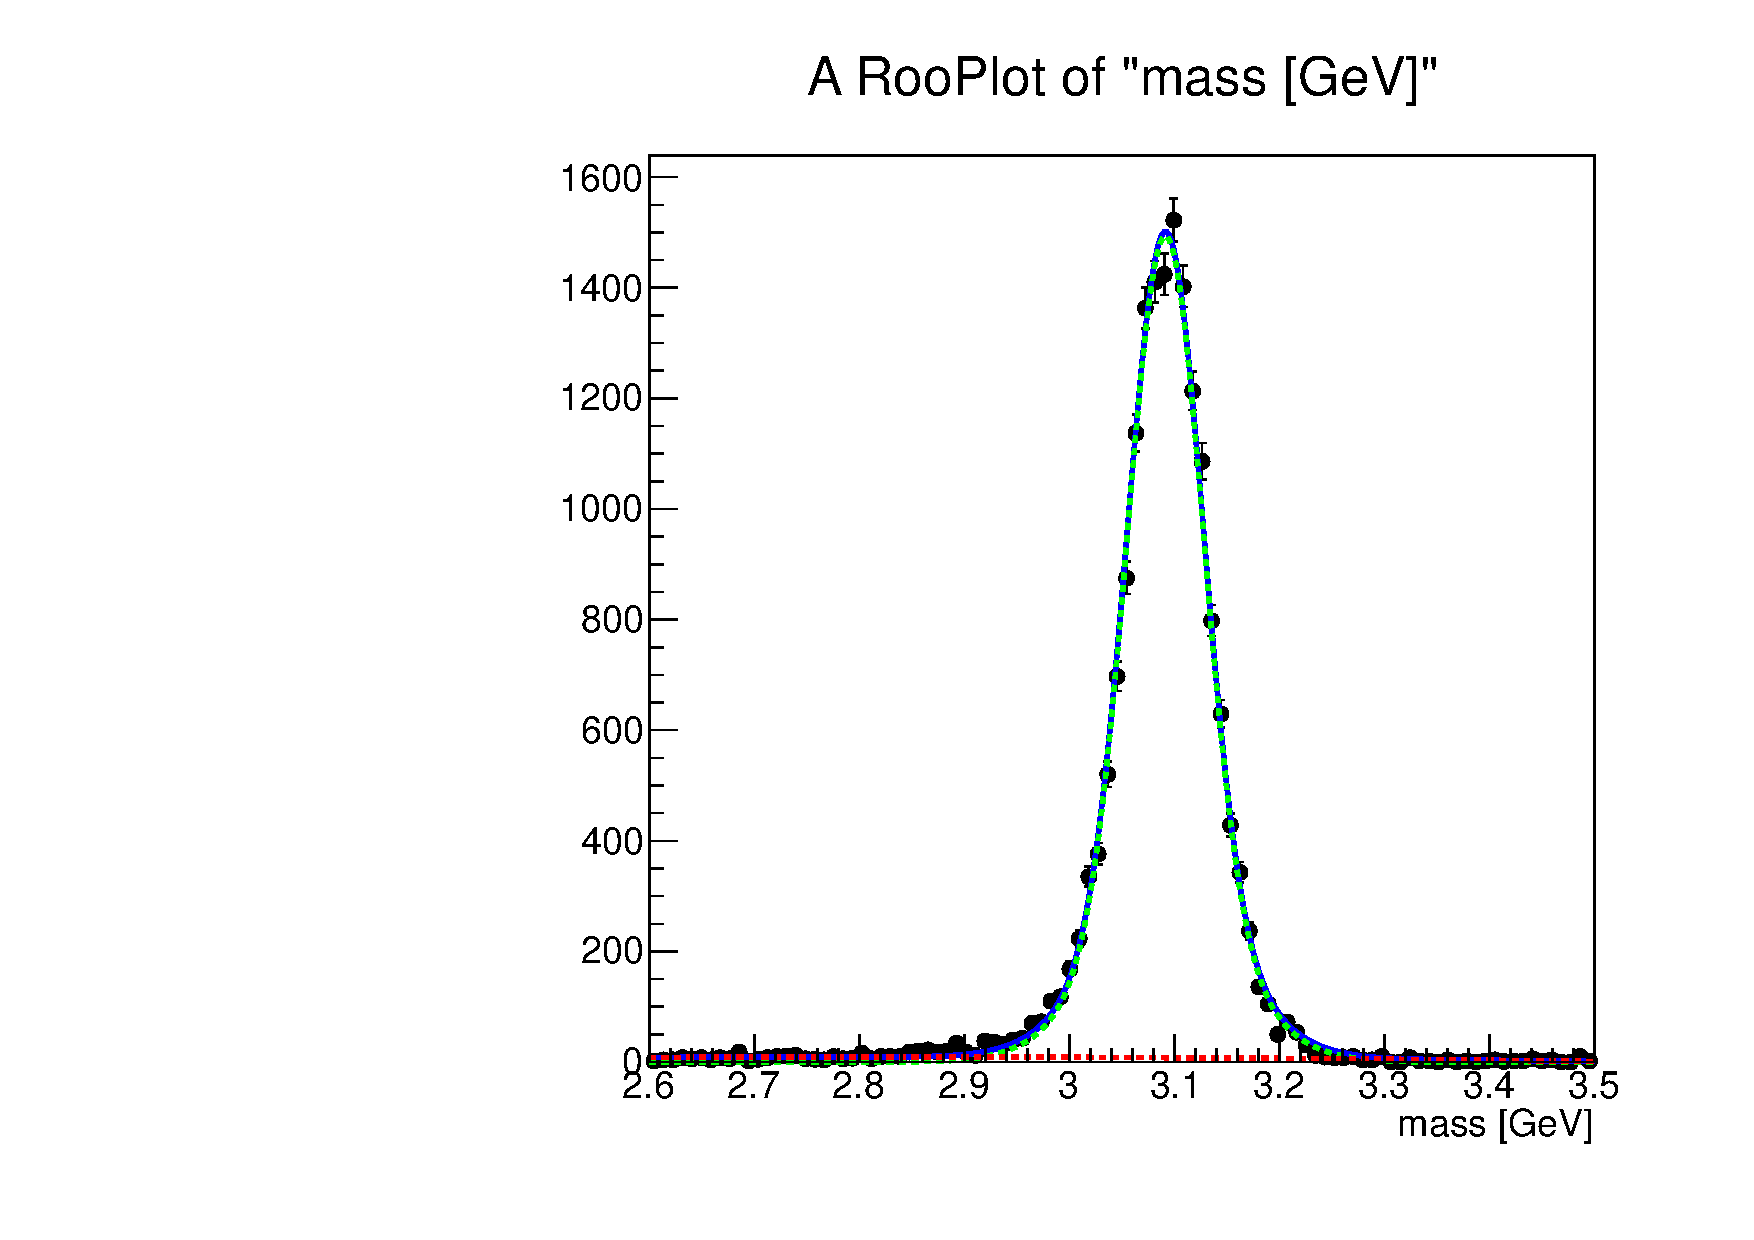
\includegraphics[width=0.25\textwidth]{../PlotsRooFitMC/croofit_trk_pass_1.pdf}
    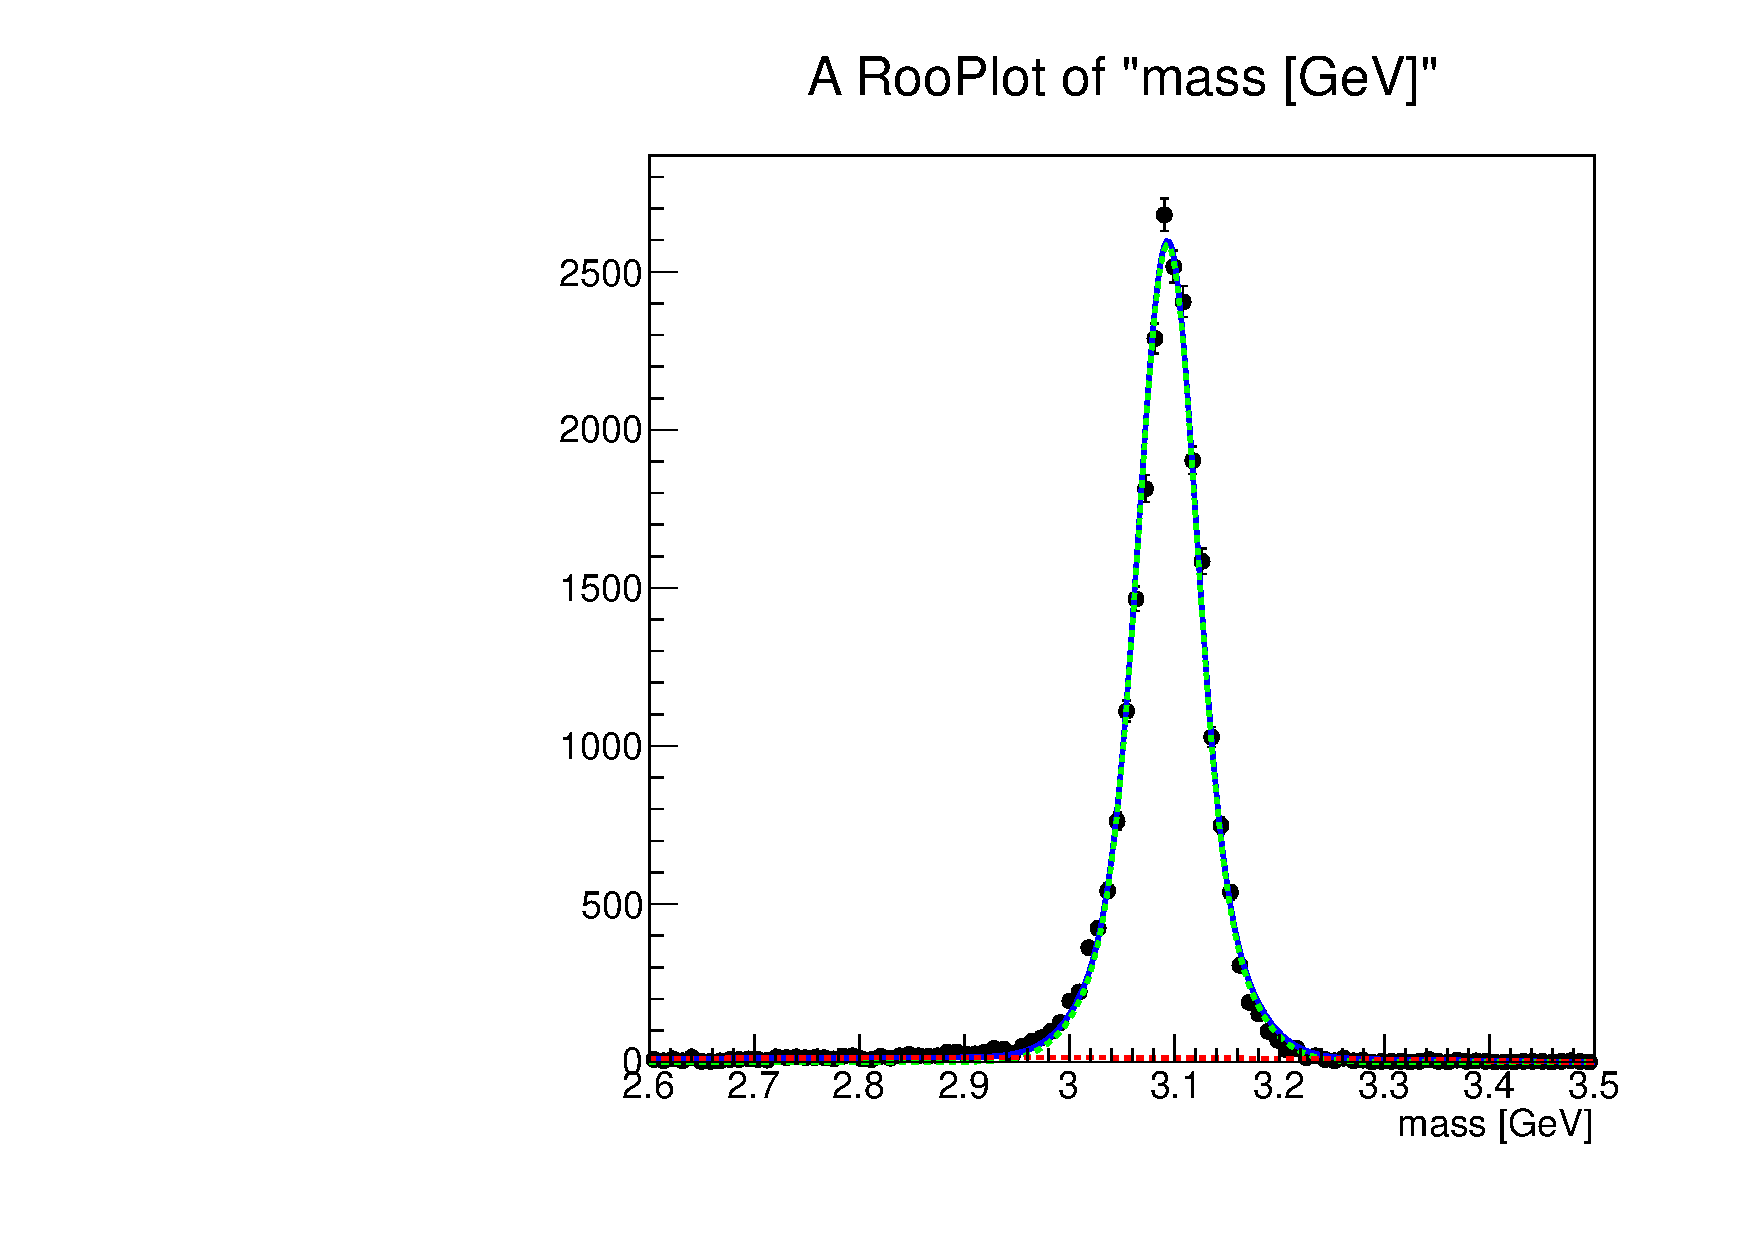
\includegraphics[width=0.25\textwidth]{../PlotsRooFitMC/croofit_trk_pass_2.pdf}
    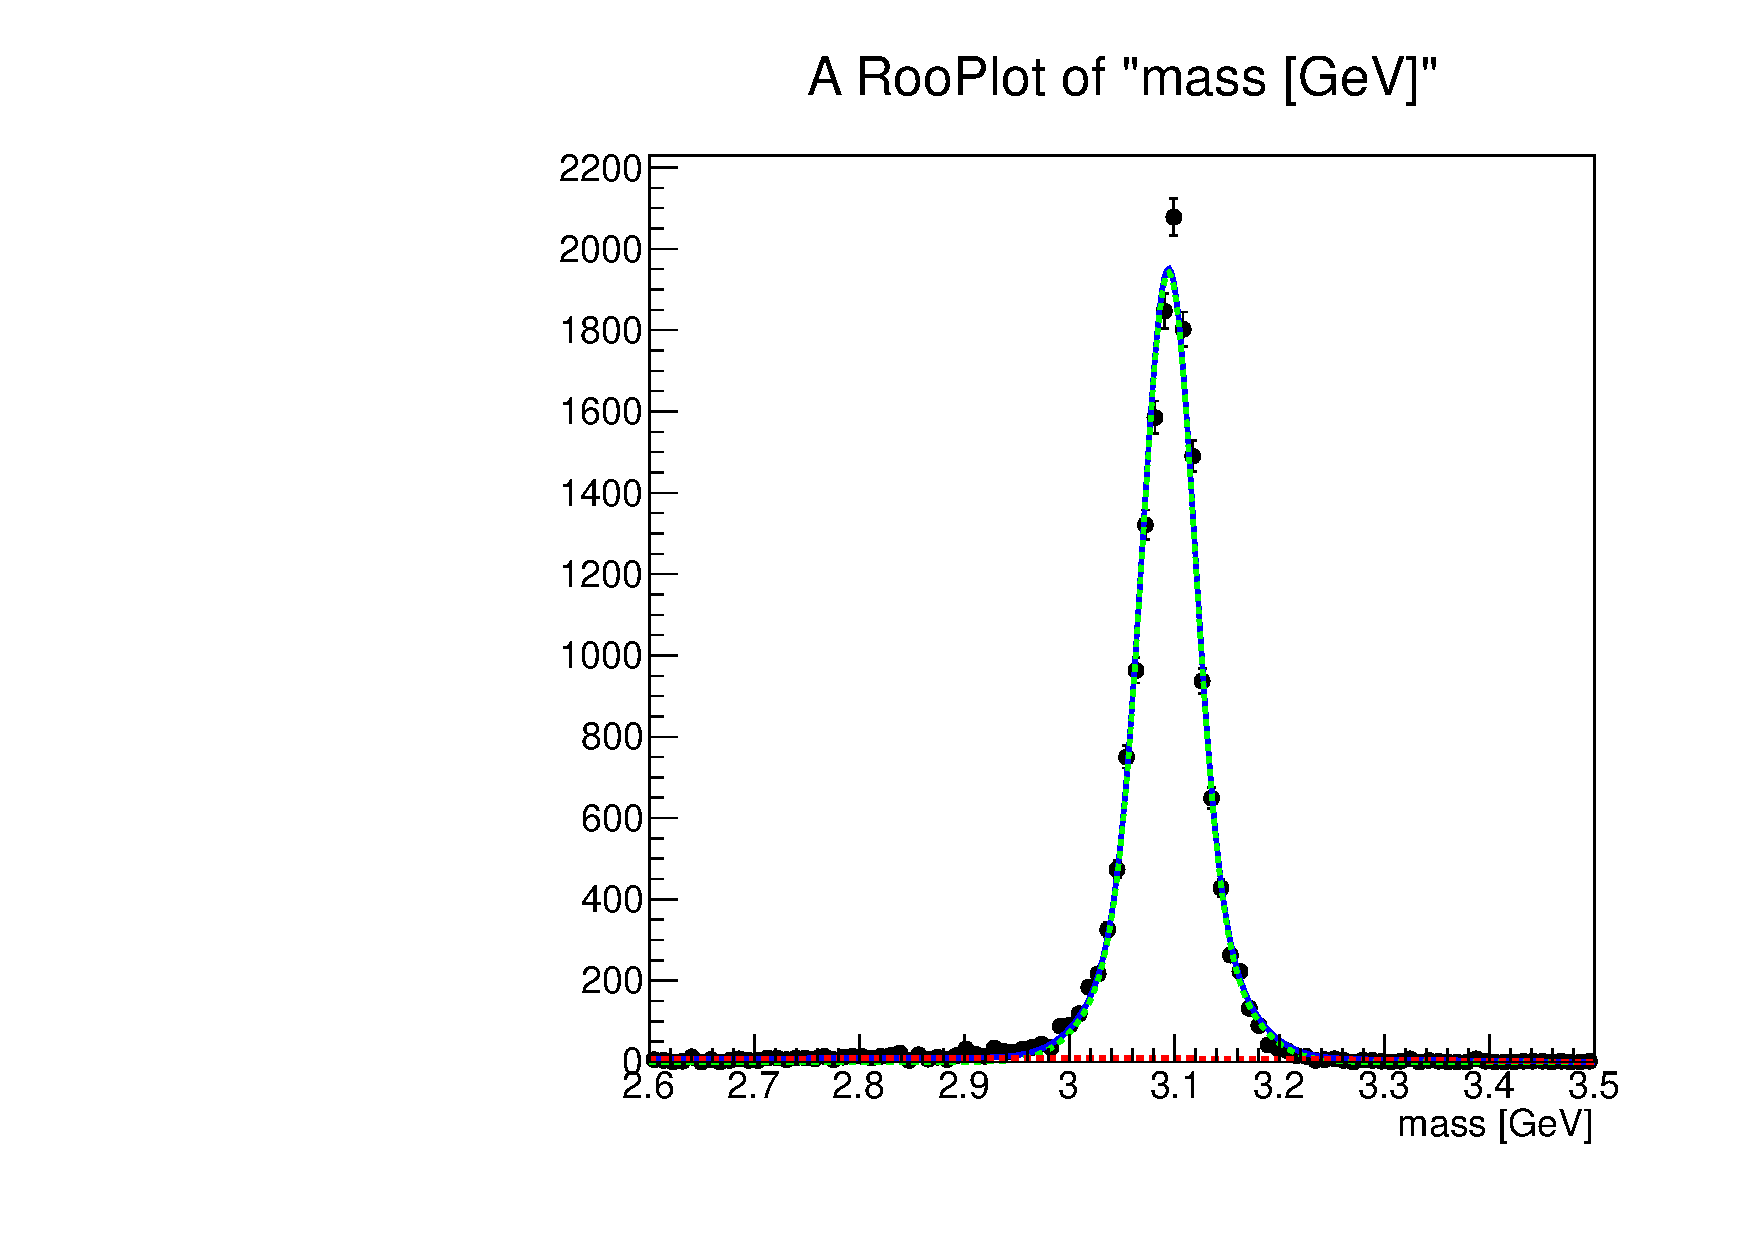
\includegraphics[width=0.25\textwidth]{../PlotsRooFitMC/croofit_trk_pass_3.pdf}
    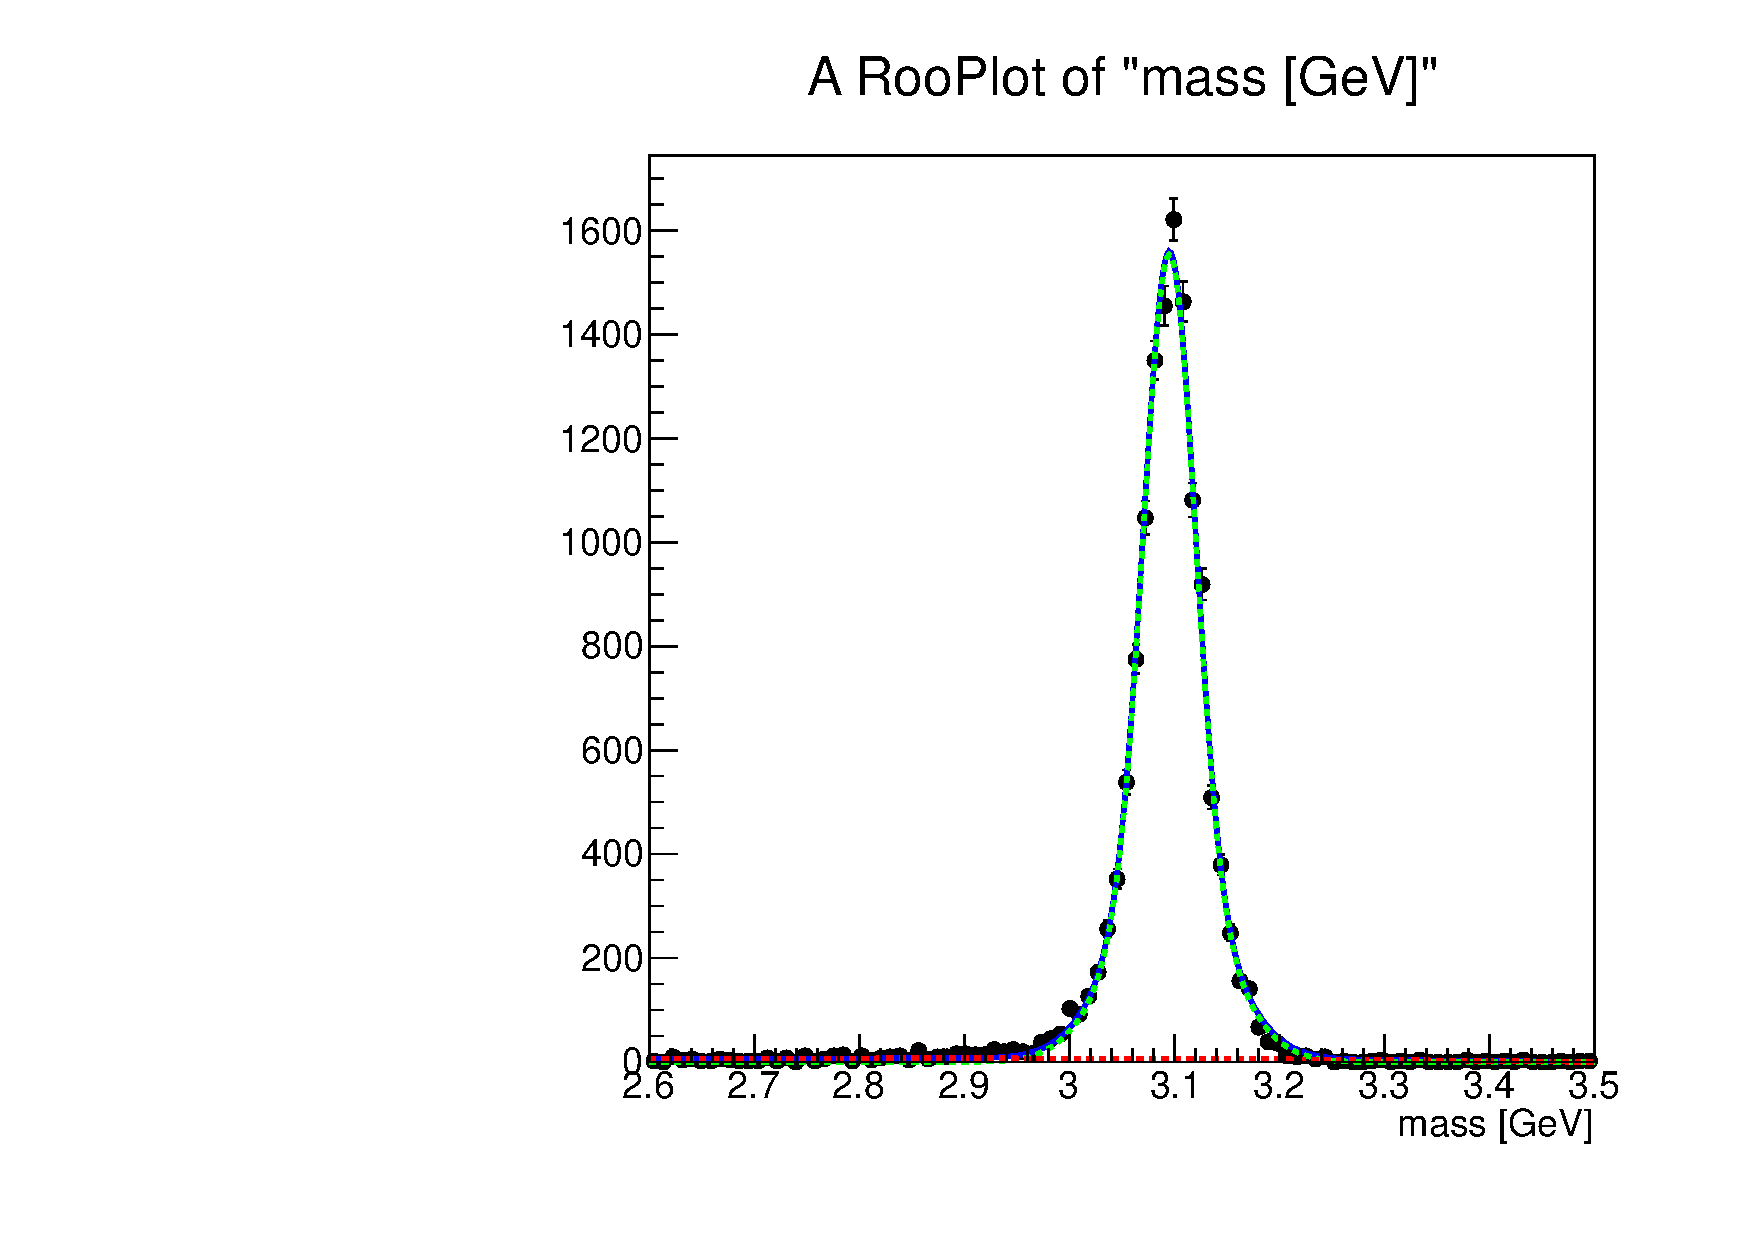
\includegraphics[width=0.25\textwidth]{../PlotsRooFitMC/croofit_trk_pass_4.pdf}
    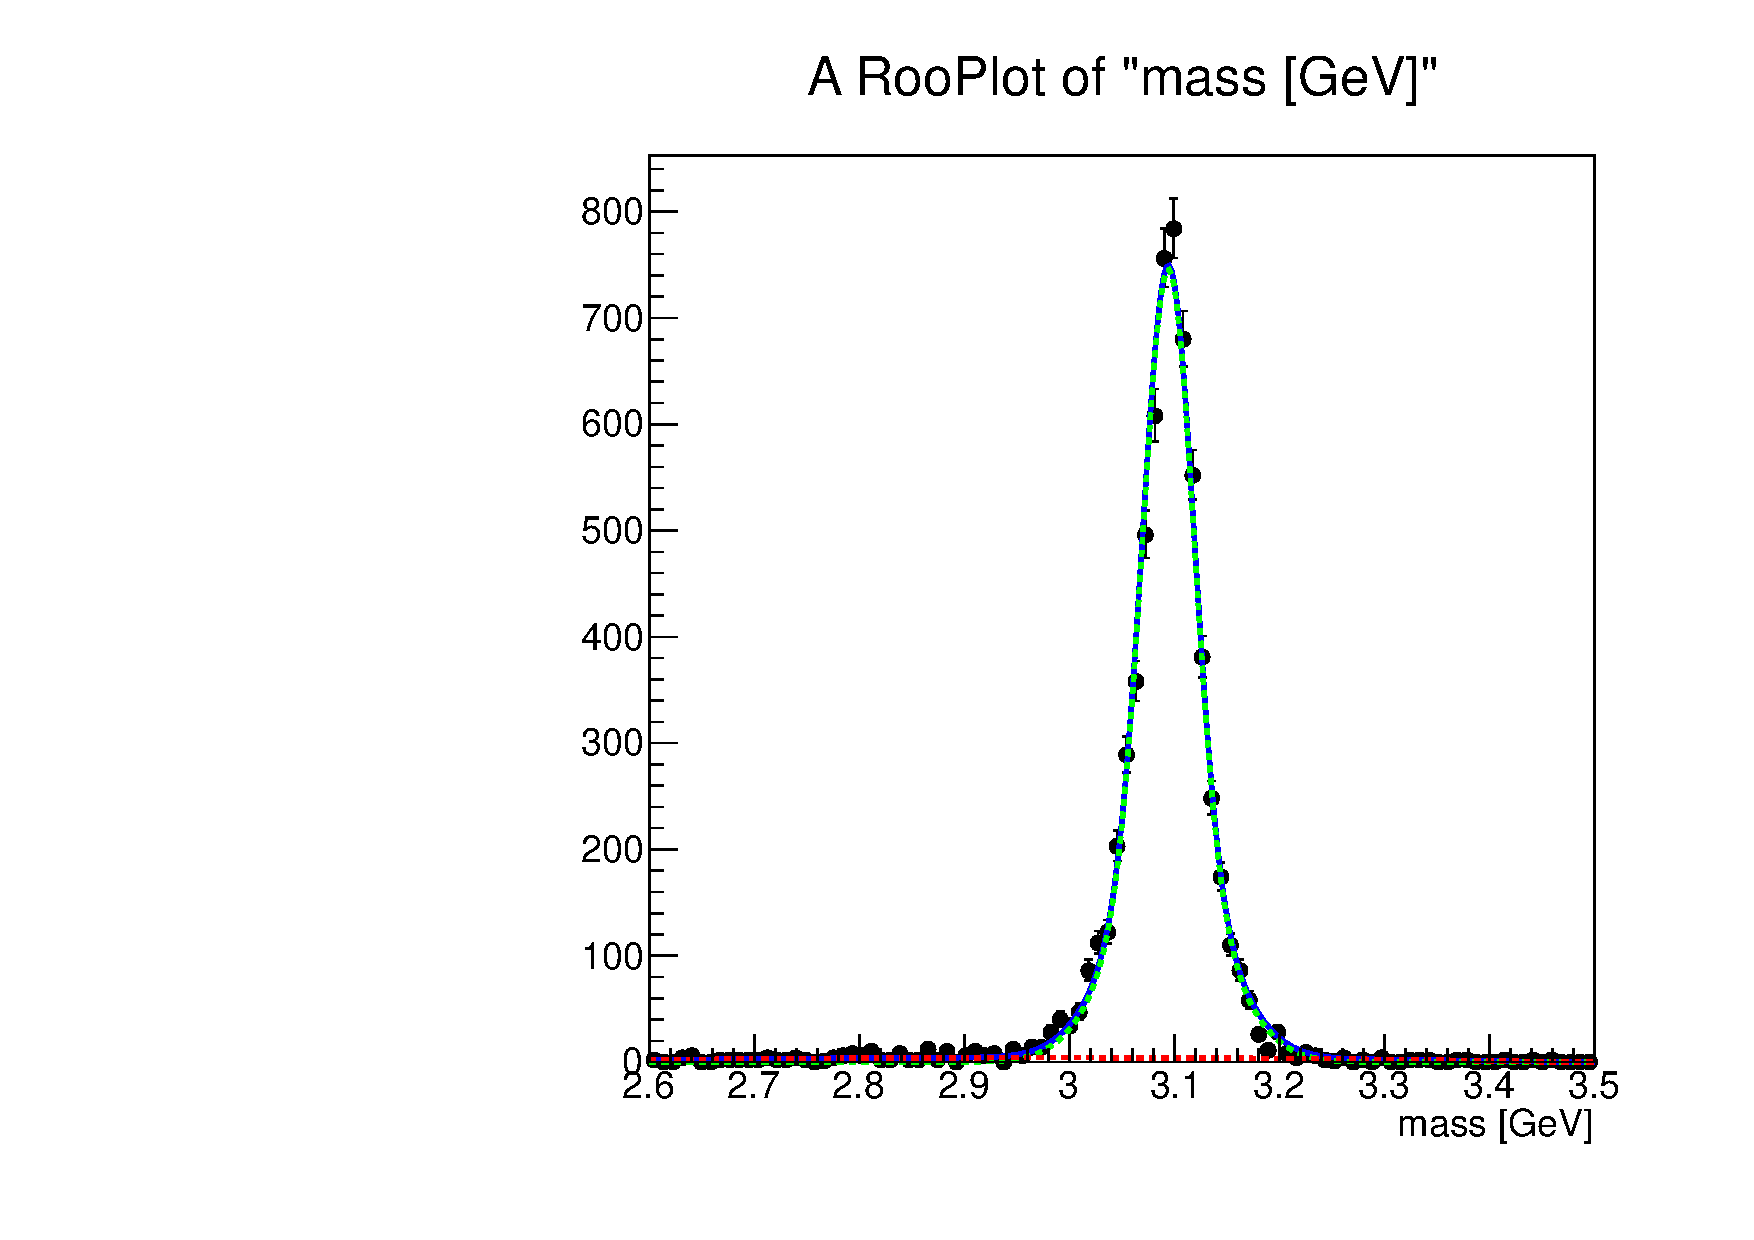
\includegraphics[width=0.25\textwidth]{../PlotsRooFitMC/croofit_trk_pass_5.pdf}
    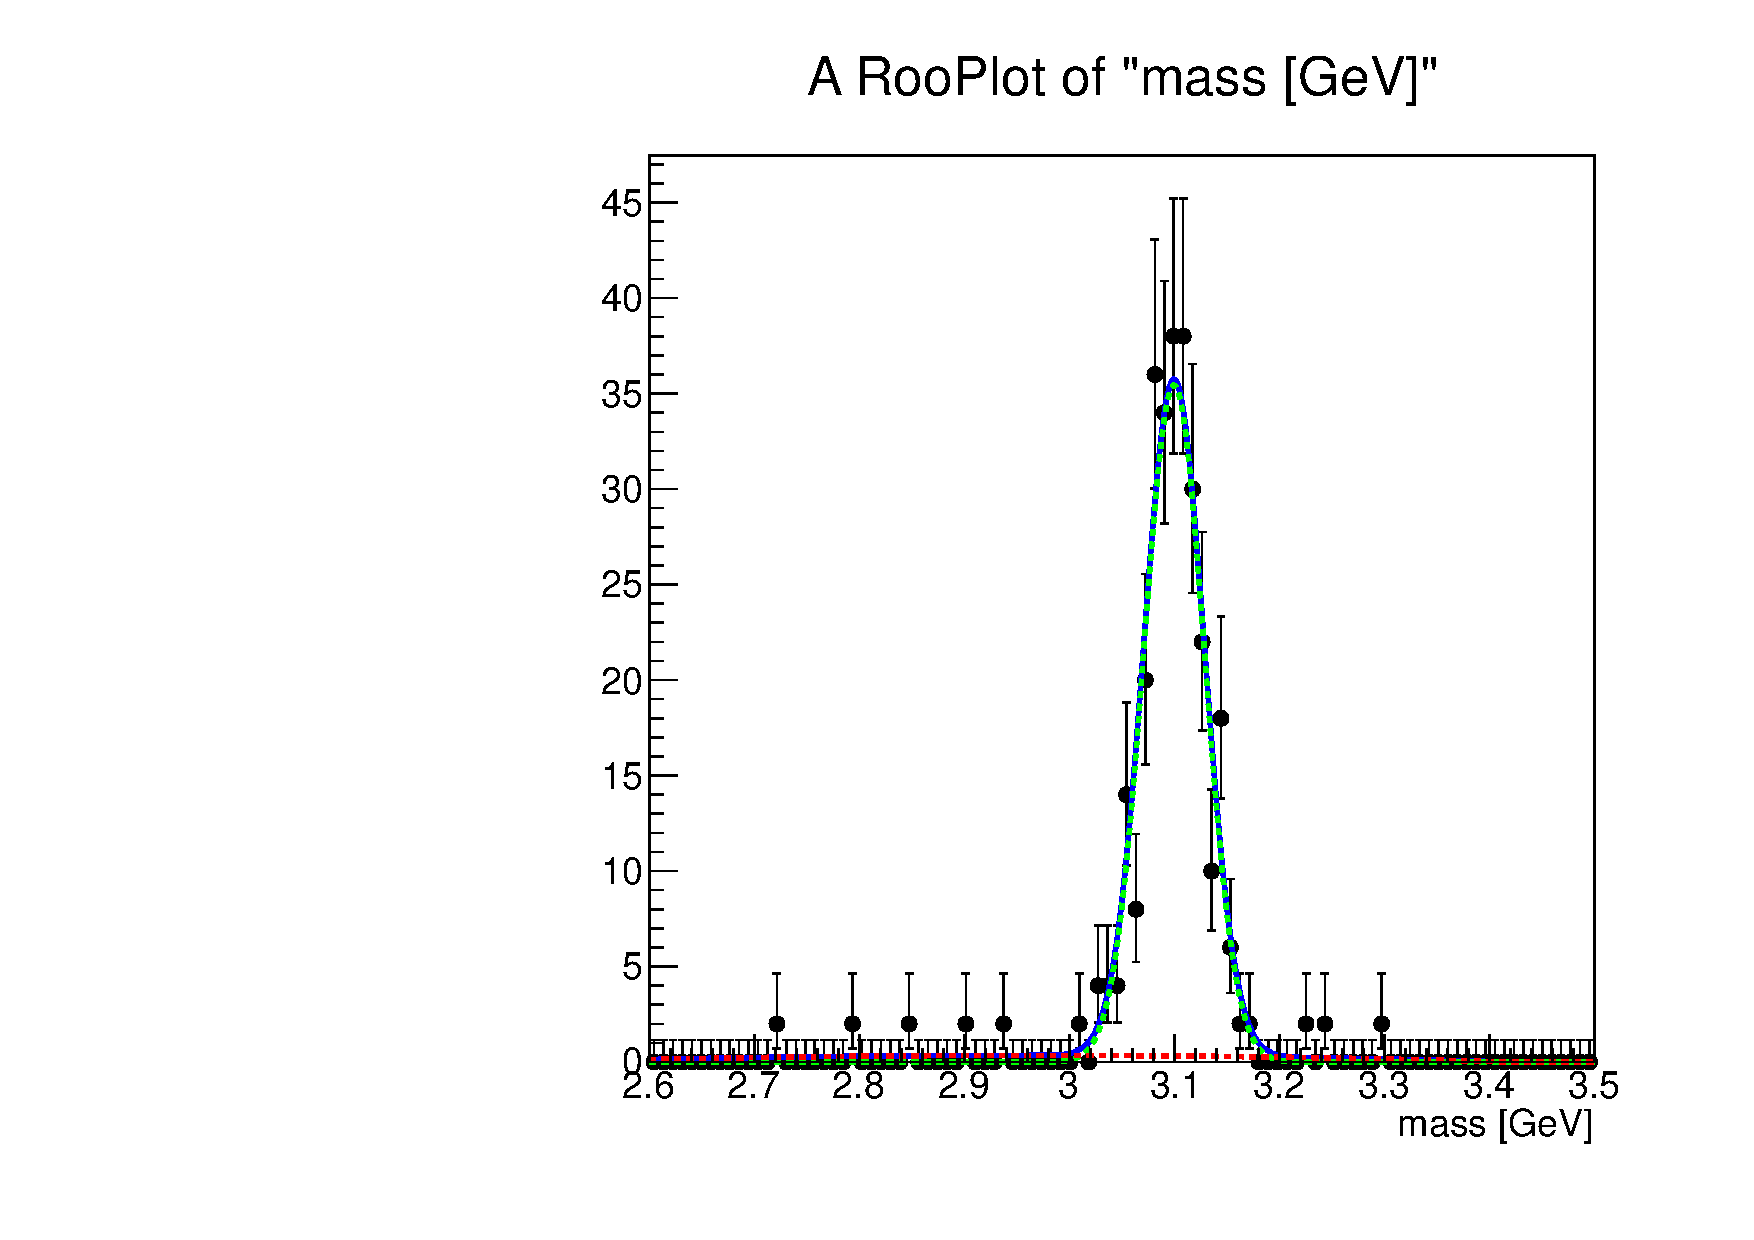
\includegraphics[width=0.25\textwidth]{../PlotsRooFitMC/croofit_trk_pass_6.pdf}
    \caption{MC Results trigger studies for passing probes, muon transverse momenta
    $\rm p_{t}$ (GeV/c)= {0.0-1.5}, {1.5-3.0}, {3.0-4.5}, {4.5-6.0}, 
    {6.0-9.0}, {9.0-20.0}, {20.0-30.0}}
   % \label{simulationfigure}
\end{figure}

\begin{figure}
    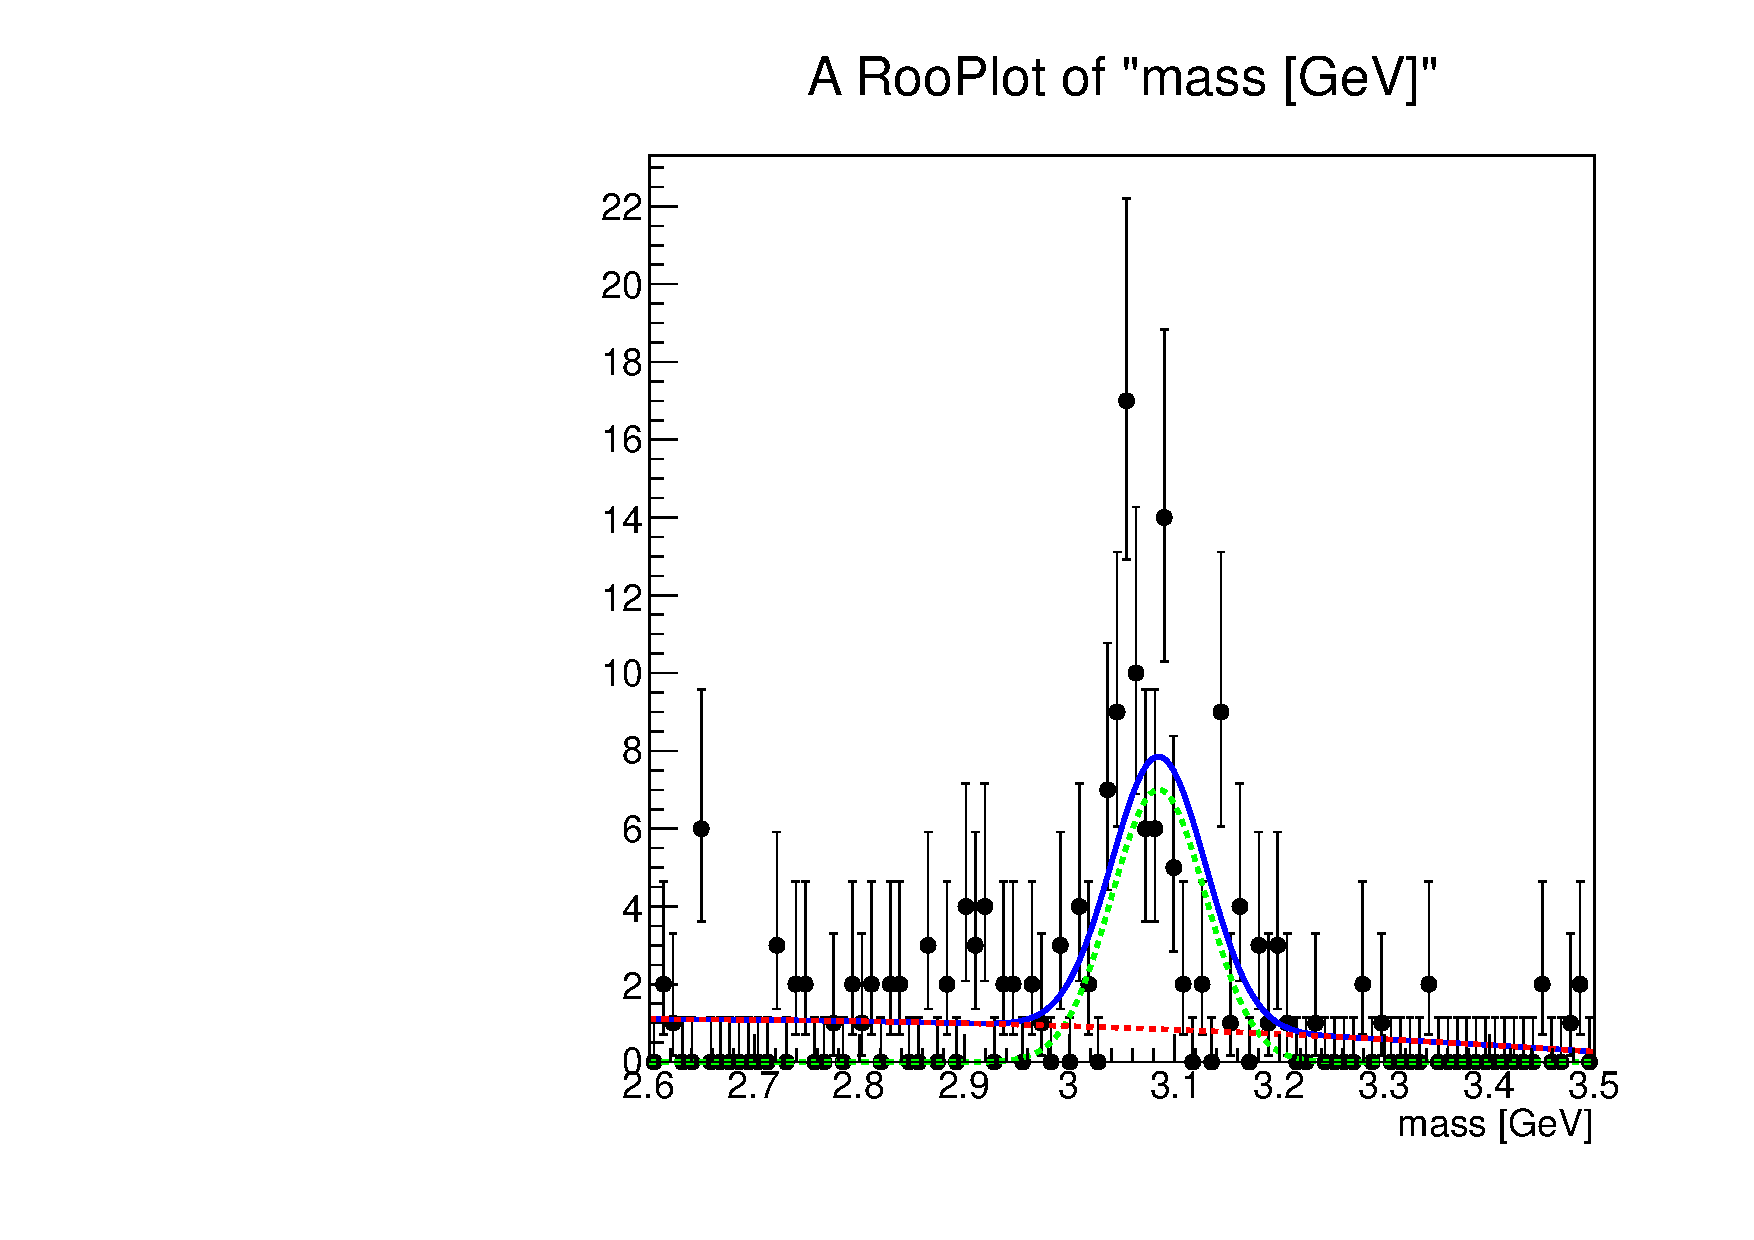
\includegraphics[width=0.25\textwidth]{../PlotsRooFitMC/croofit_trk_fail_0.pdf}
    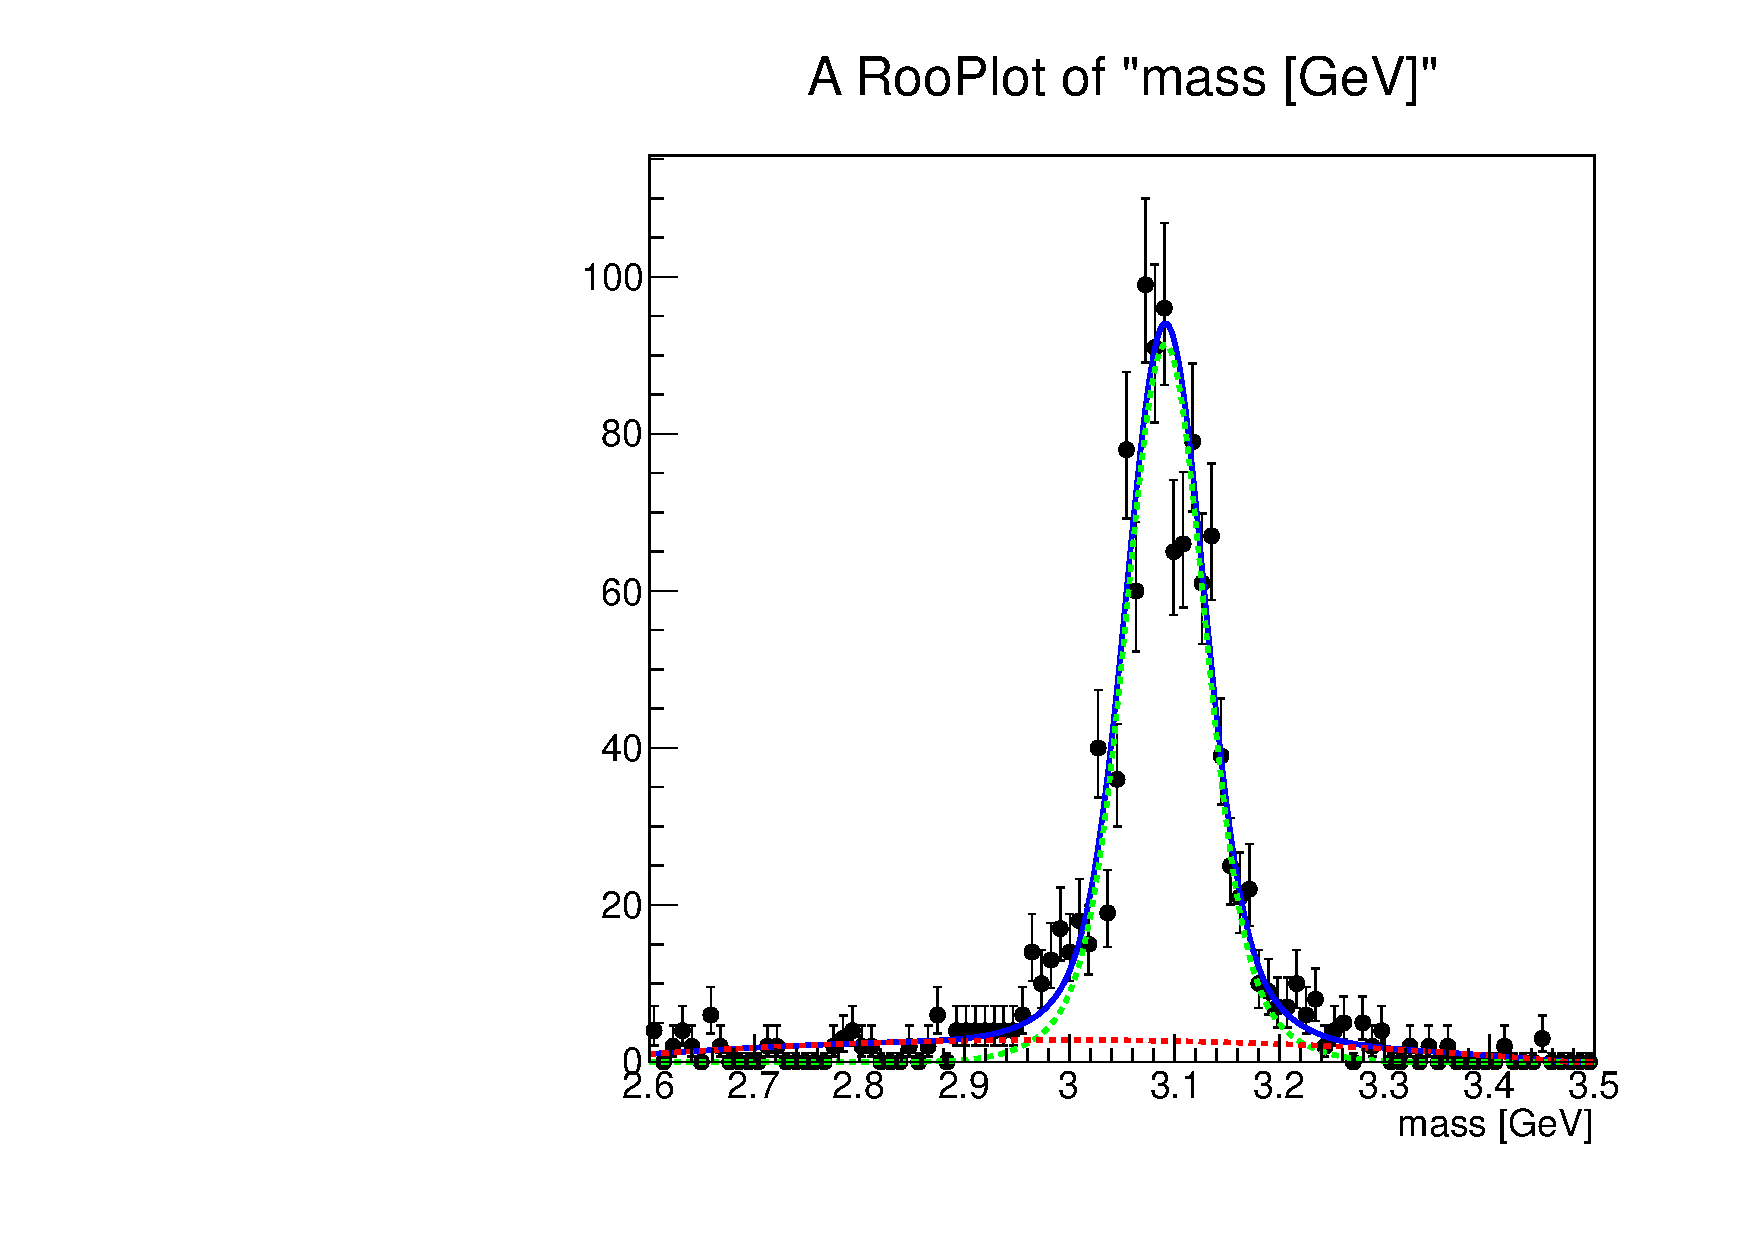
\includegraphics[width=0.25\textwidth]{../PlotsRooFitMC/croofit_trk_fail_1.pdf}
    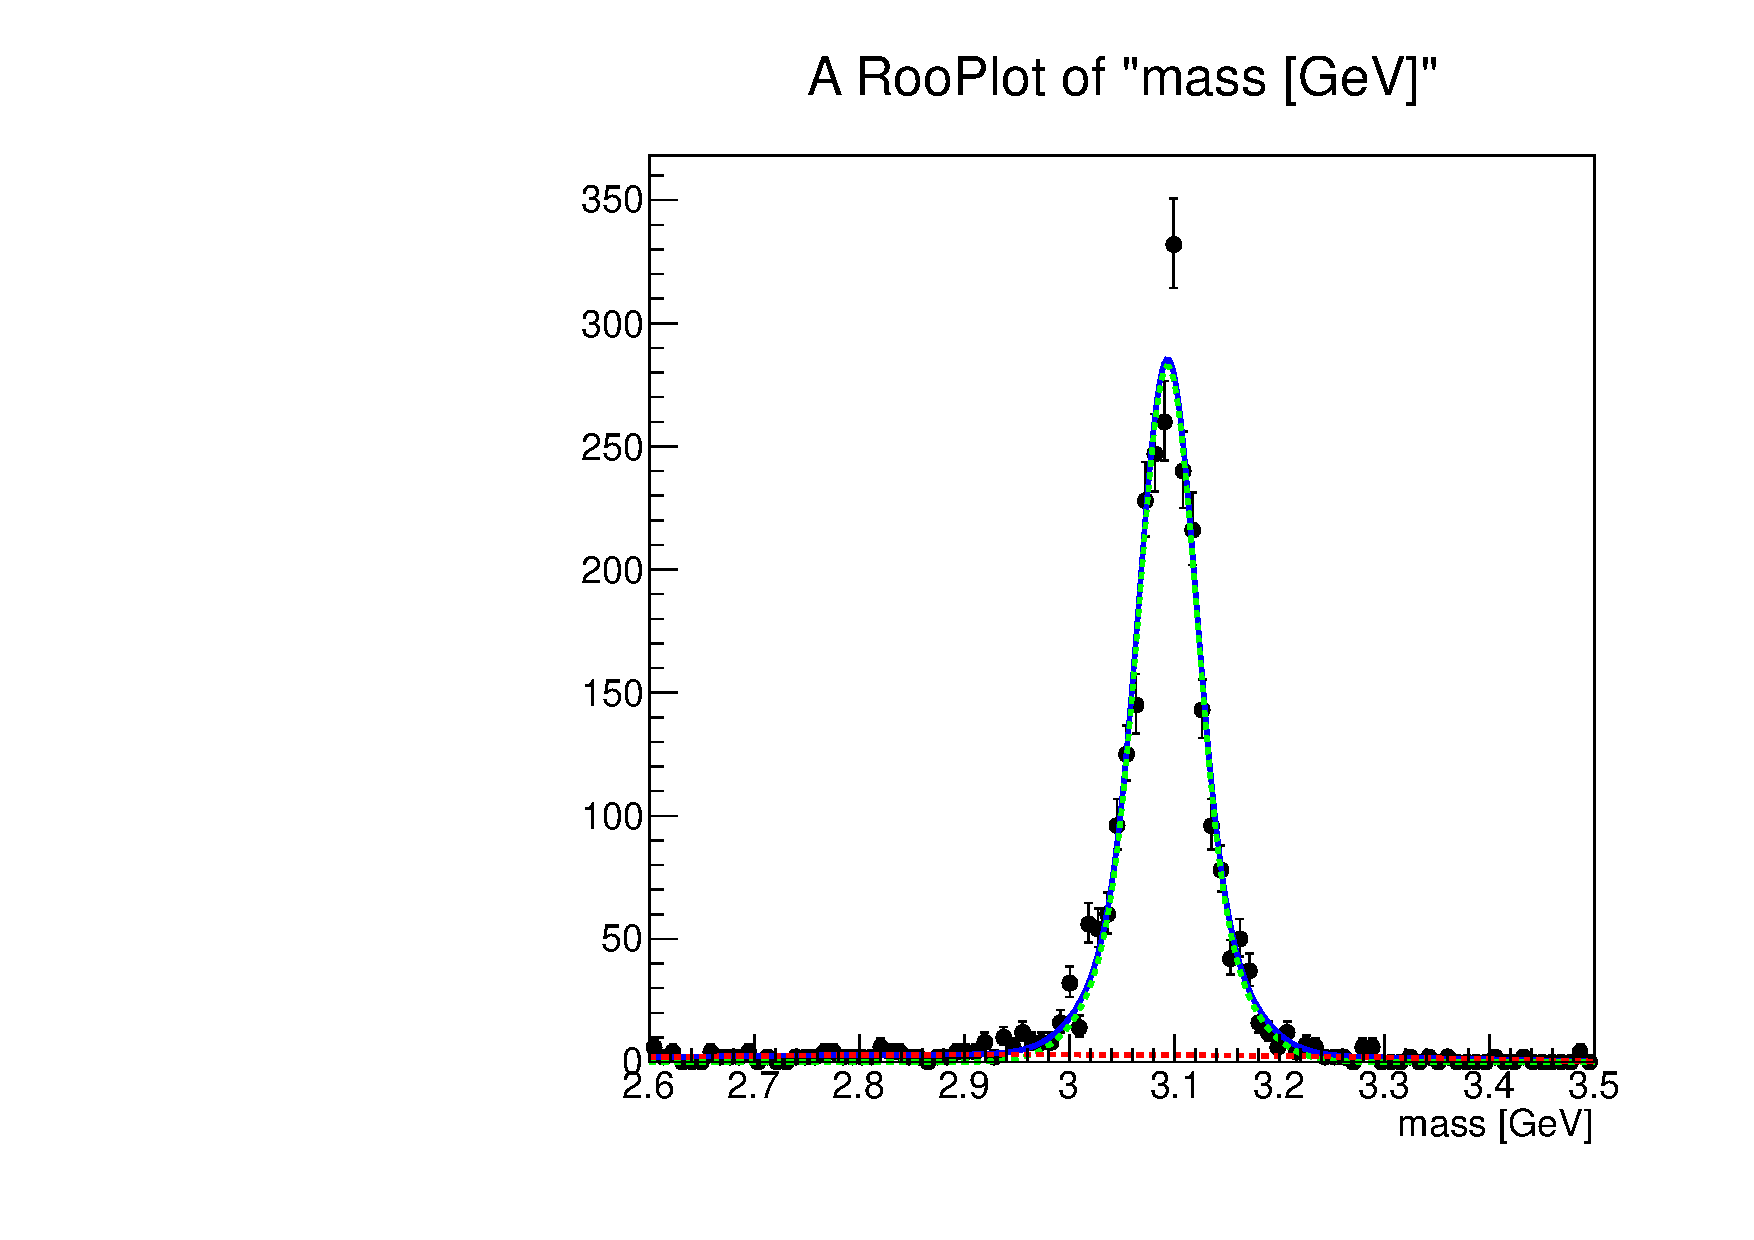
\includegraphics[width=0.25\textwidth]{../PlotsRooFitMC/croofit_trk_fail_2.pdf}
    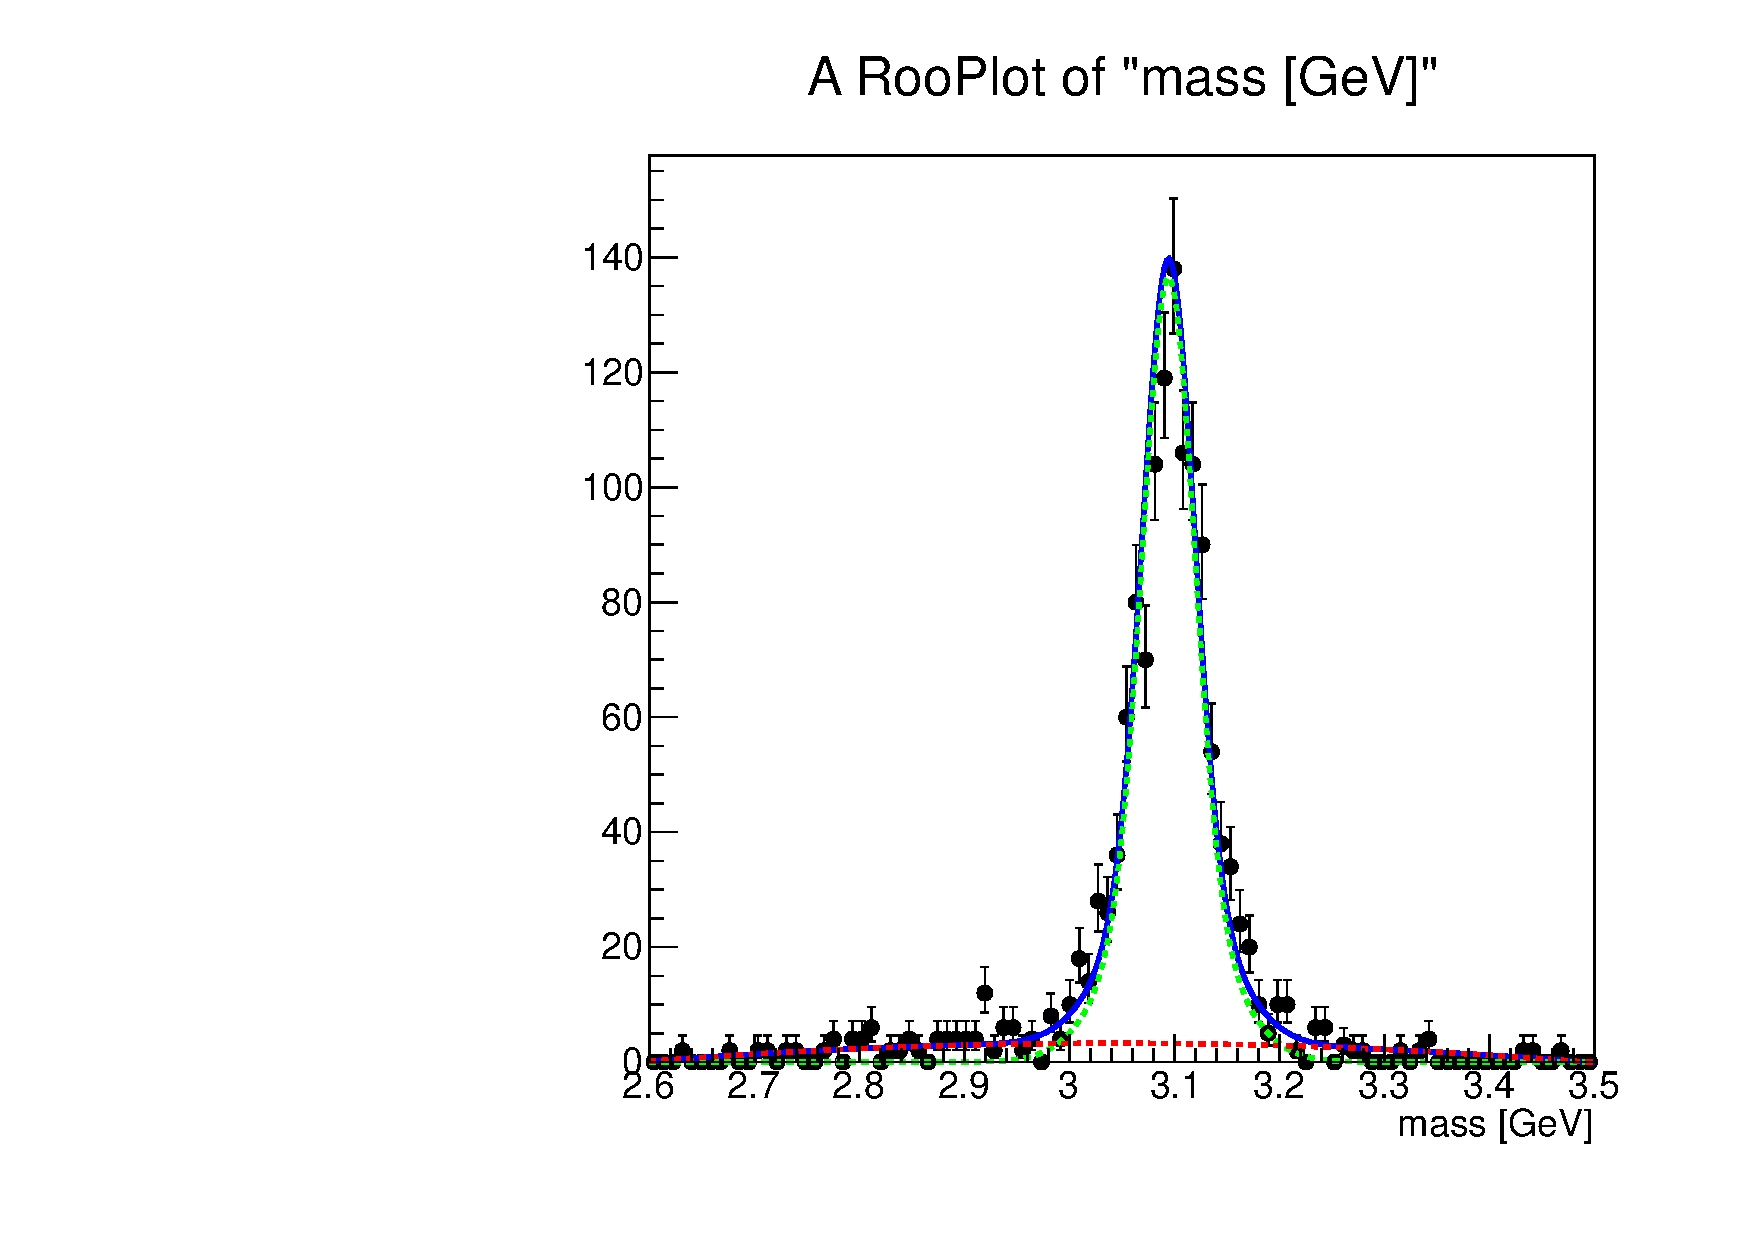
\includegraphics[width=0.25\textwidth]{../PlotsRooFitMC/croofit_trk_fail_3.pdf}
    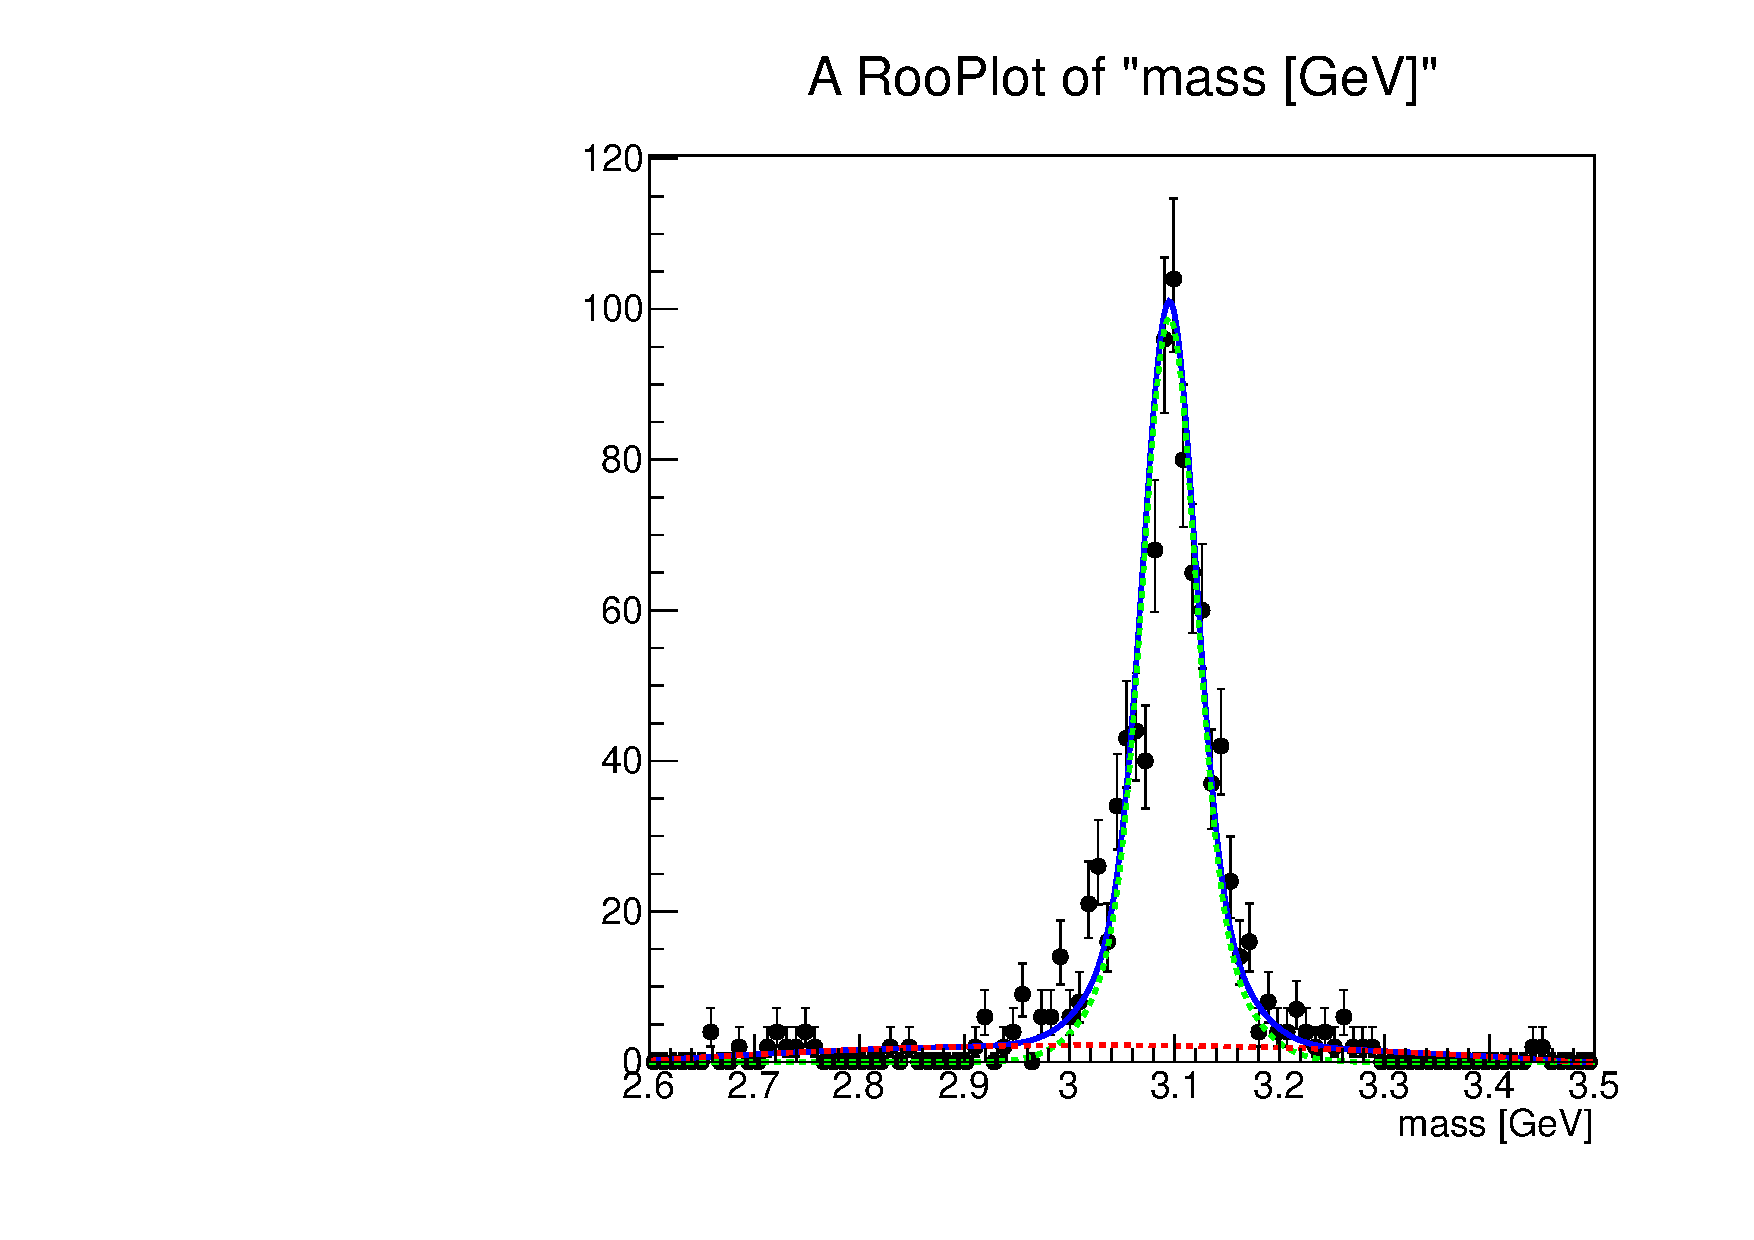
\includegraphics[width=0.25\textwidth]{../PlotsRooFitMC/croofit_trk_fail_4.pdf}
    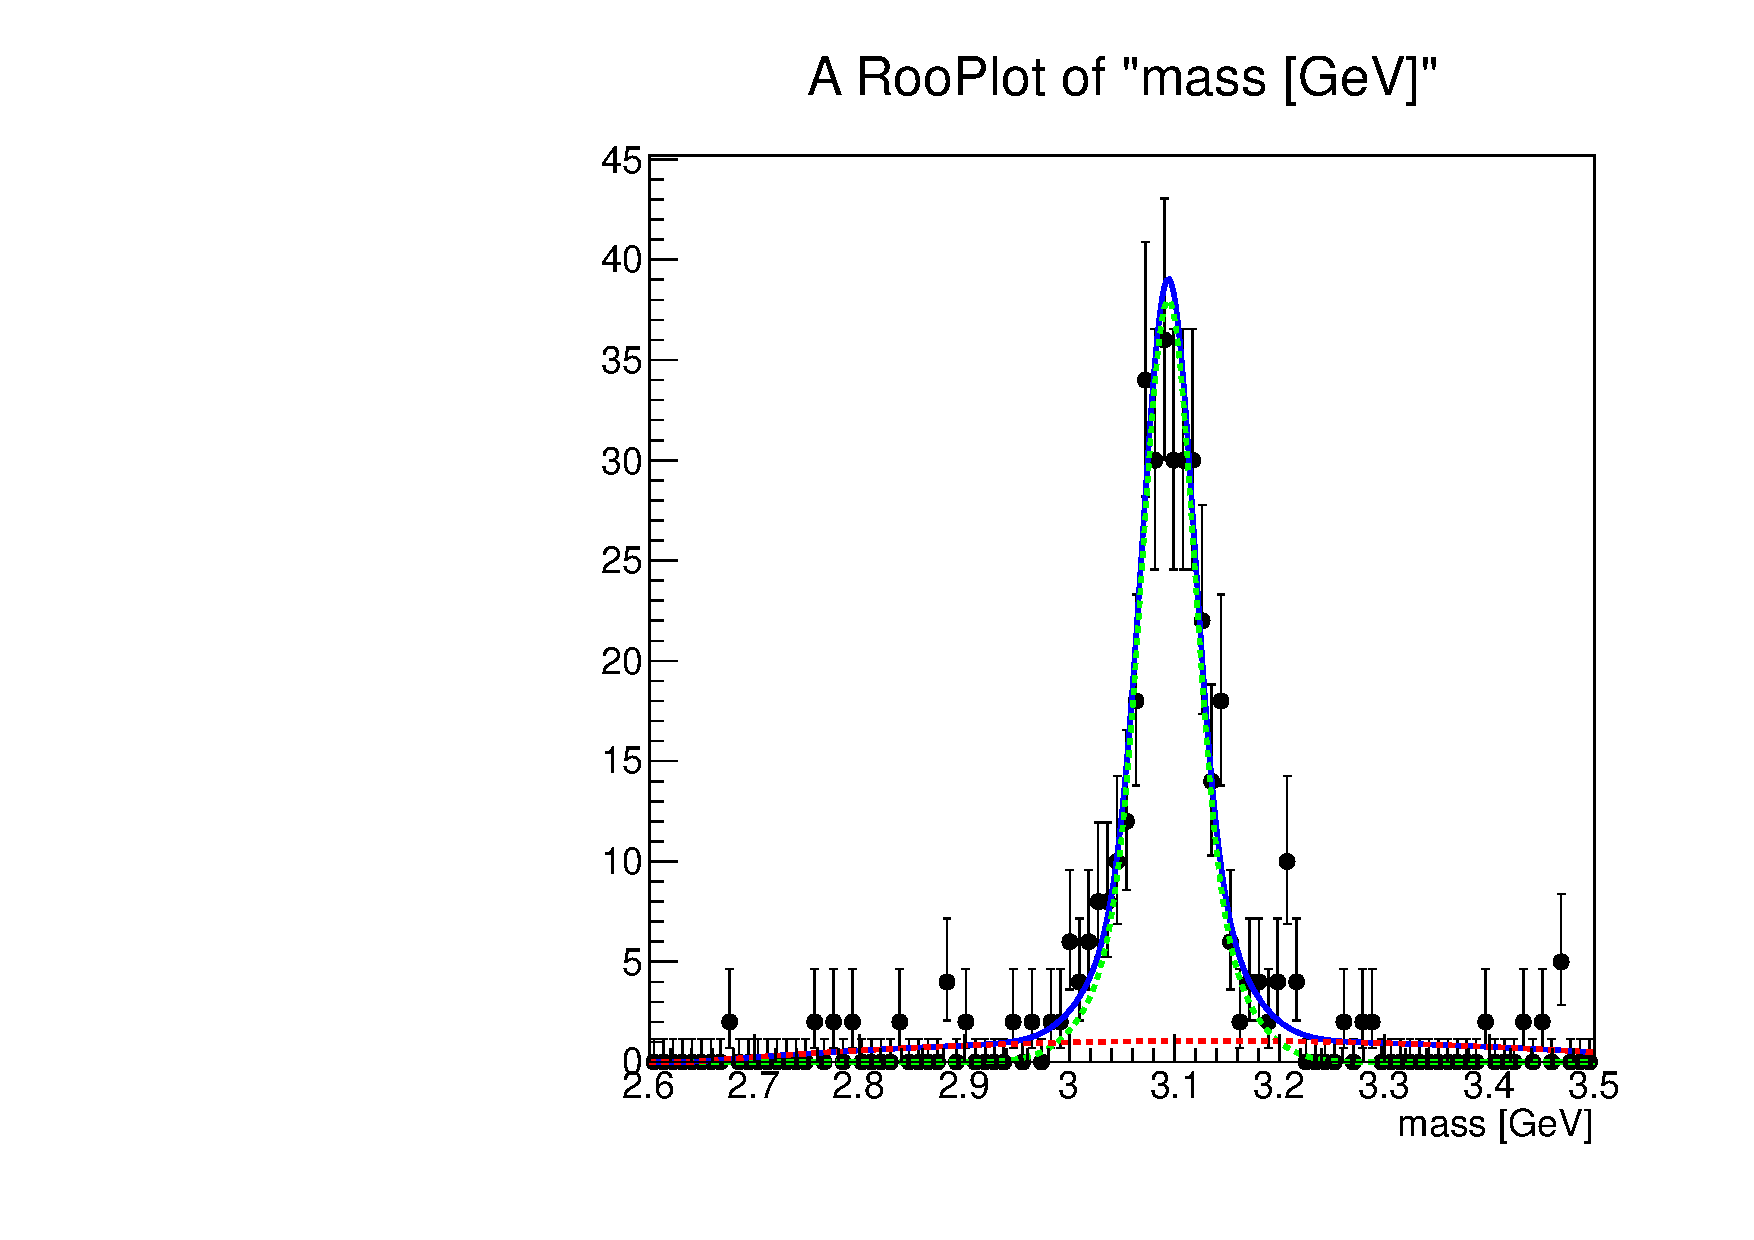
\includegraphics[width=0.25\textwidth]{../PlotsRooFitMC/croofit_trk_fail_5.pdf}
    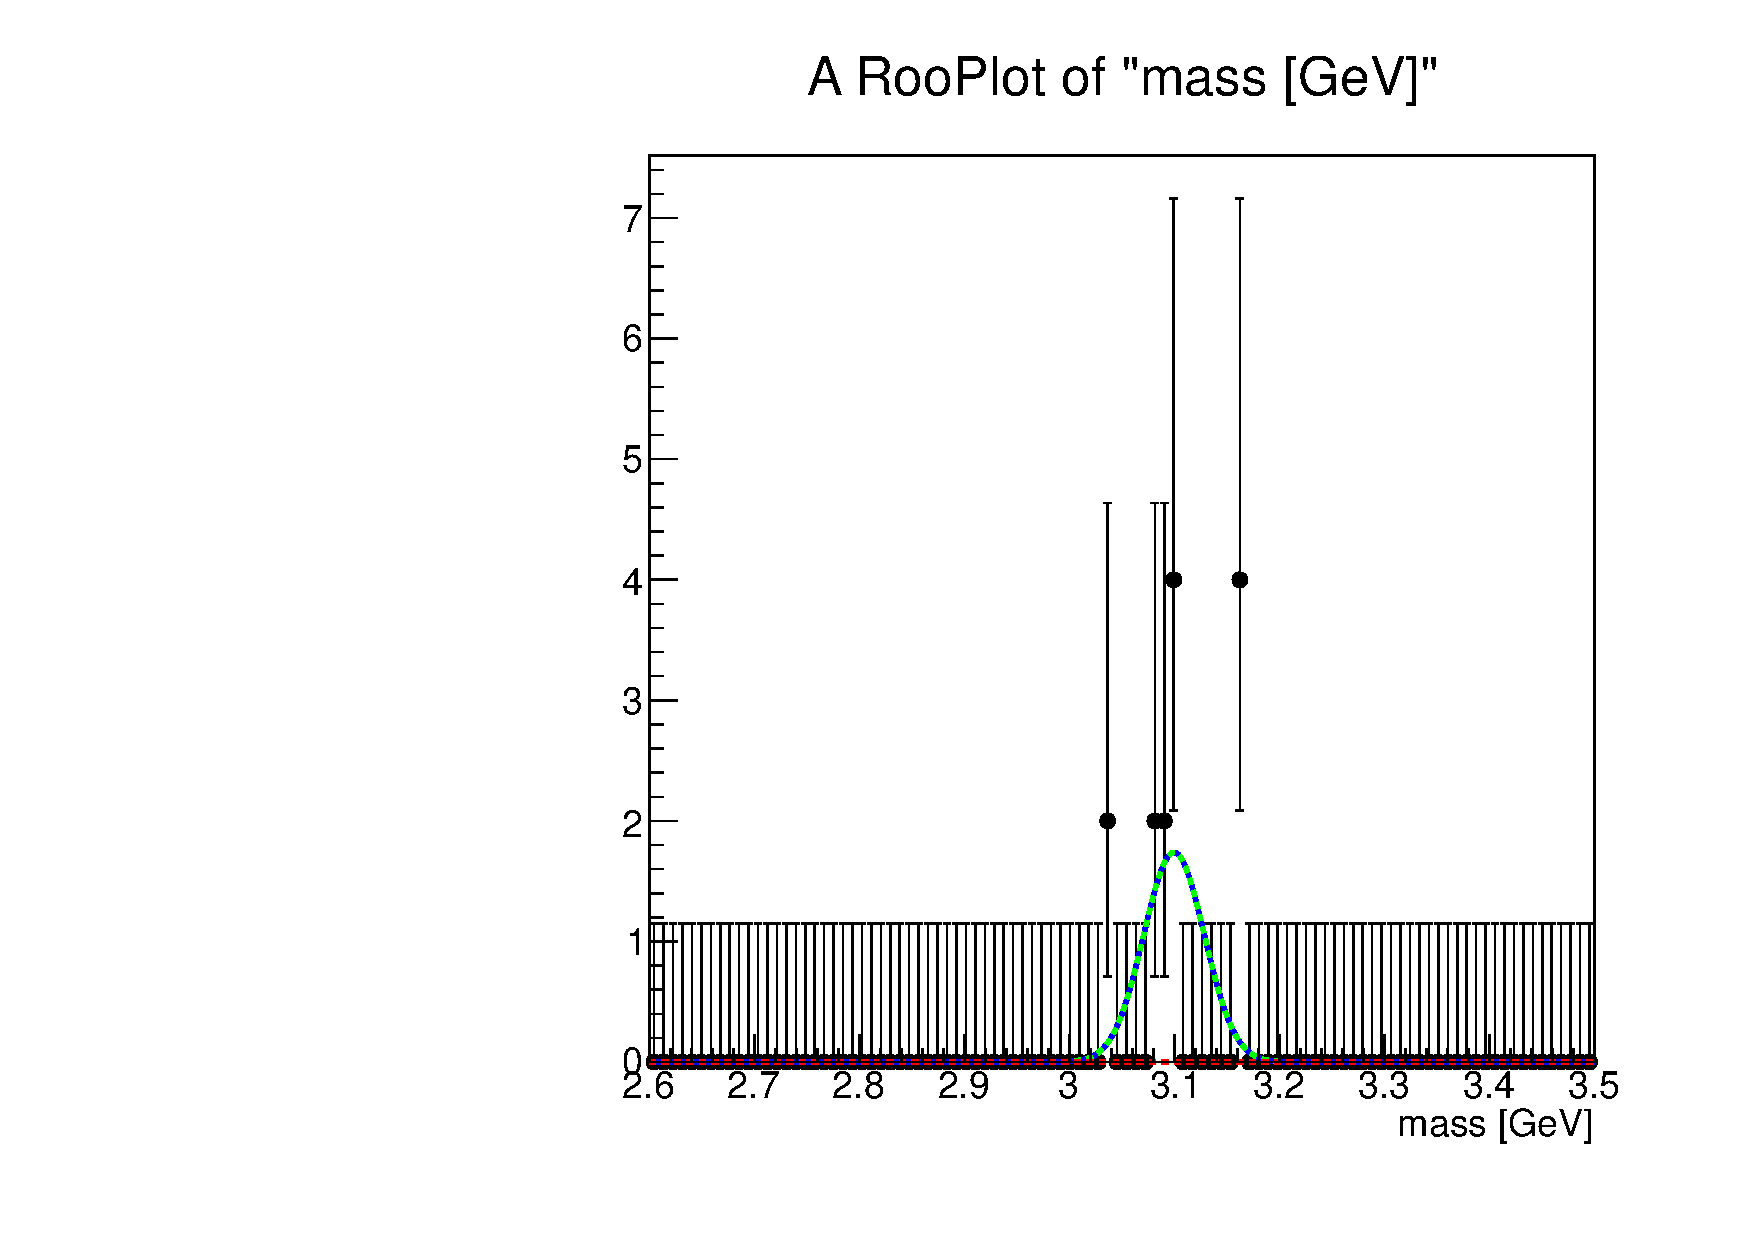
\includegraphics[width=0.25\textwidth]{../PlotsRooFitMC/croofit_trk_fail_6.pdf}
    \caption{MC Results tracking studies for failing probes, muon transverse momenta
    $\rm p_{t}$ (GeV/c)= {0.0-1.5}, {1.5-3.0}, {3.0-4.5}, {4.5-6.0}, 
    {6.0-9.0}, {9.0-20.0}, {20.0-30.0}}
   % \label{simulationfigure}
\end{figure}

\begin{figure}
    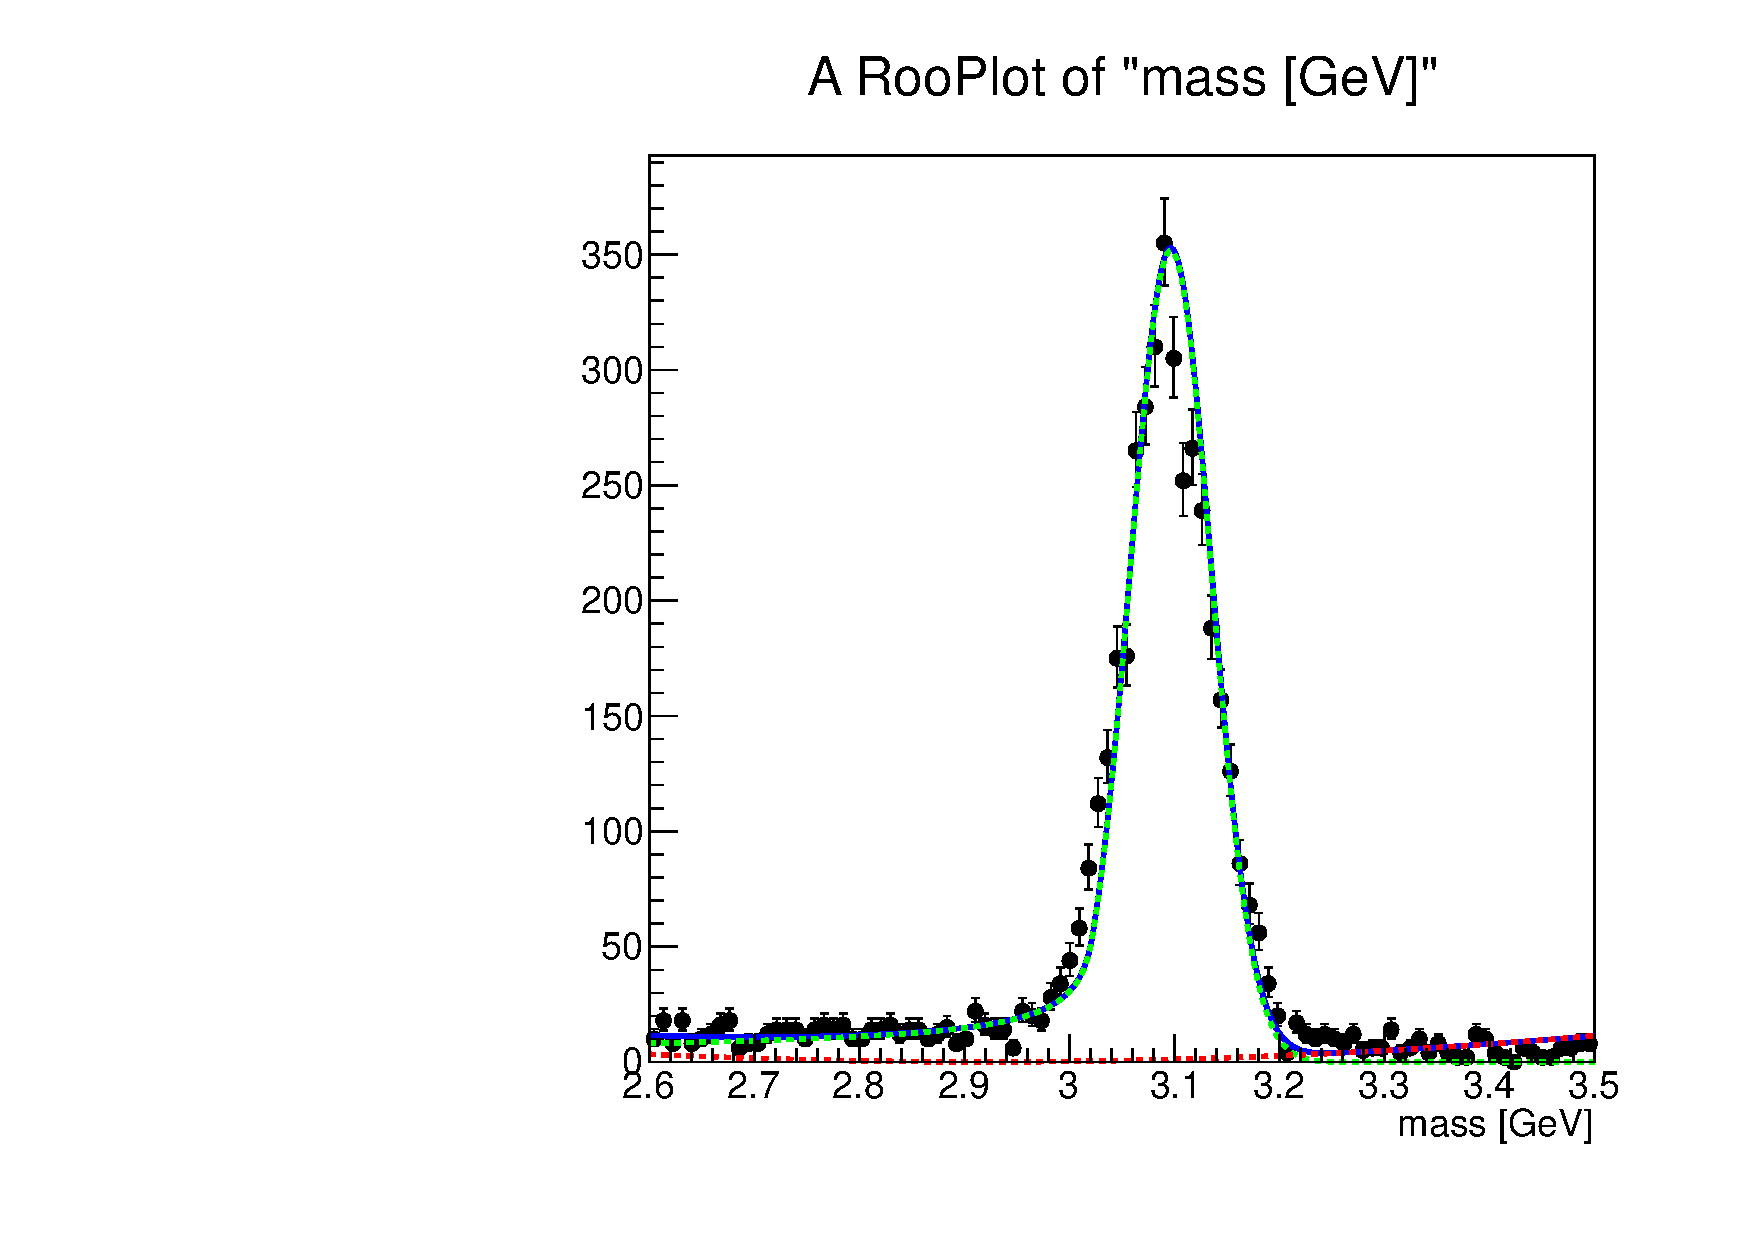
\includegraphics[width=0.25\textwidth]{../PlotsRooFitMC/croofit_id_pass_0.pdf}
    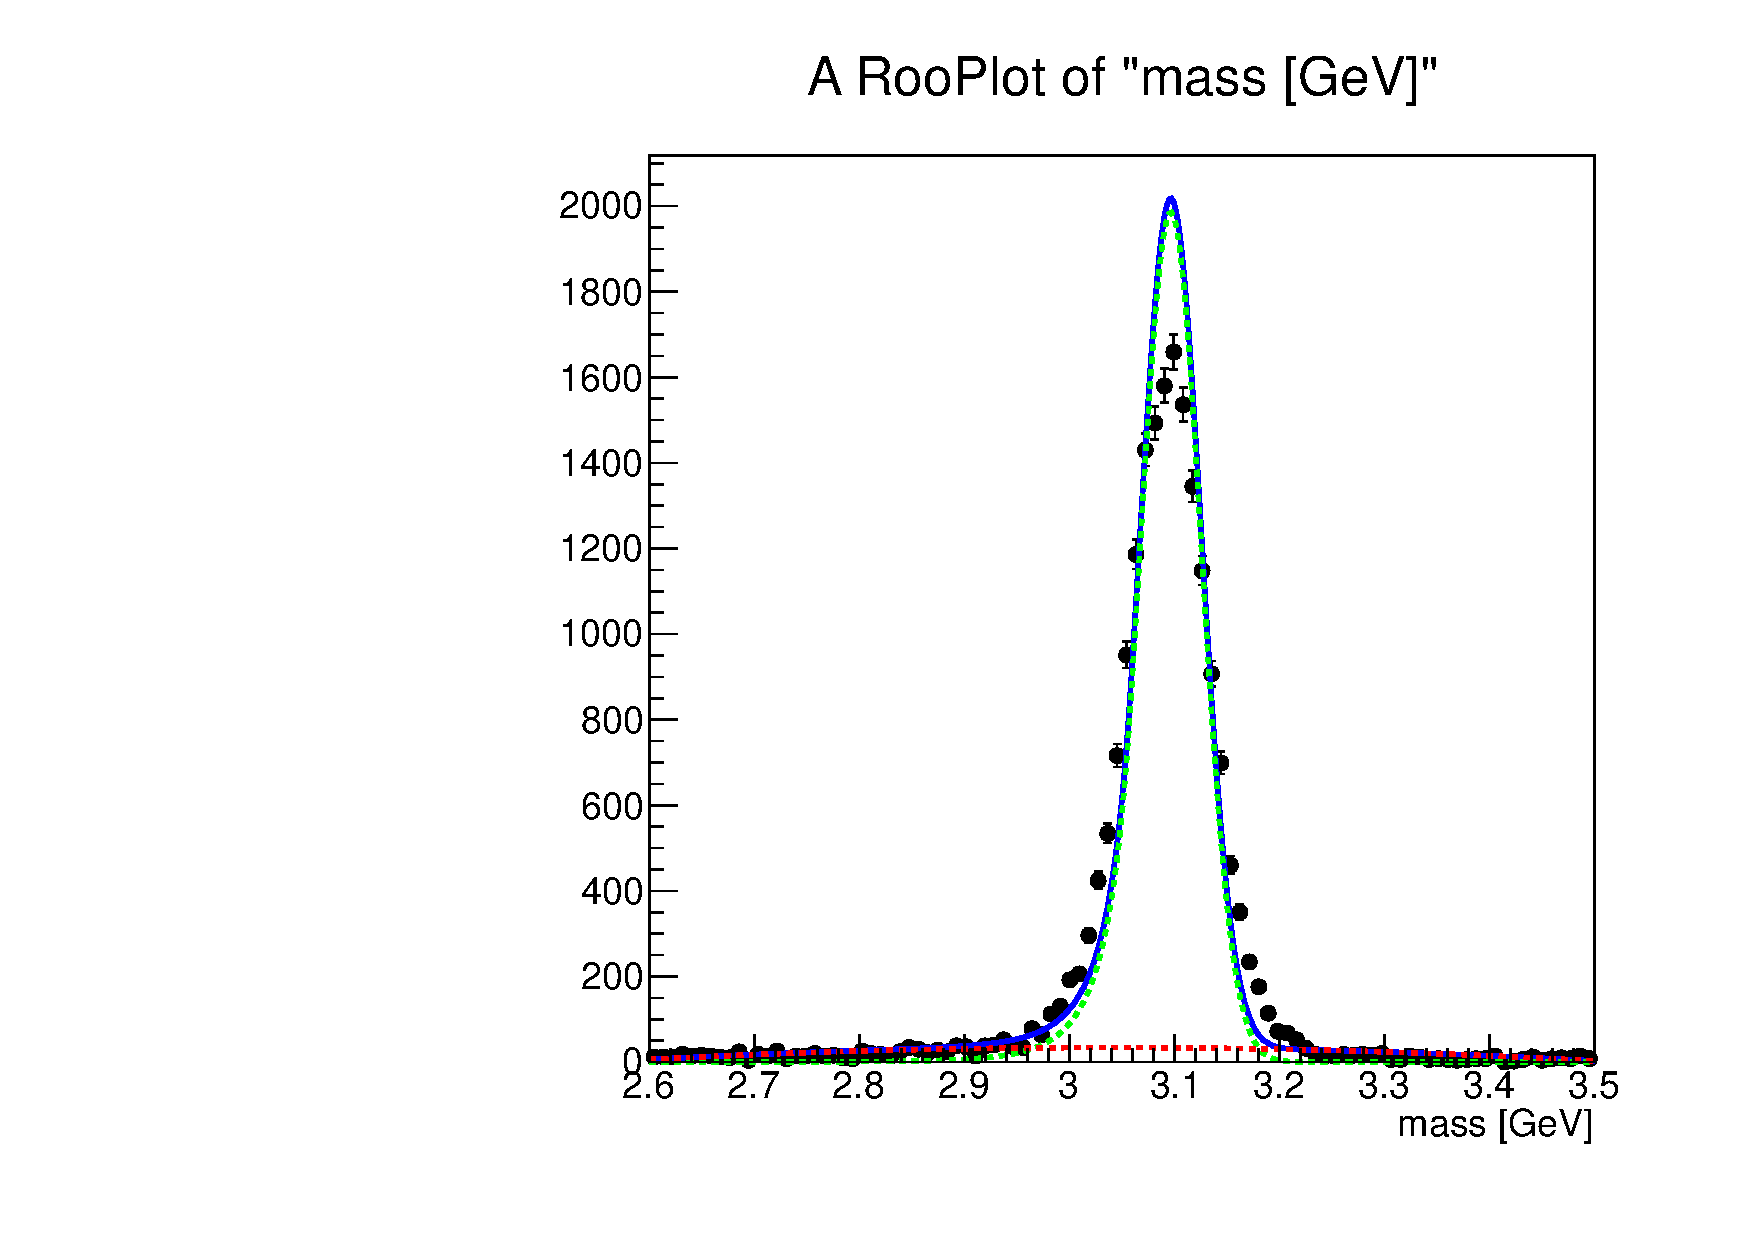
\includegraphics[width=0.25\textwidth]{../PlotsRooFitMC/croofit_id_pass_1.pdf}
    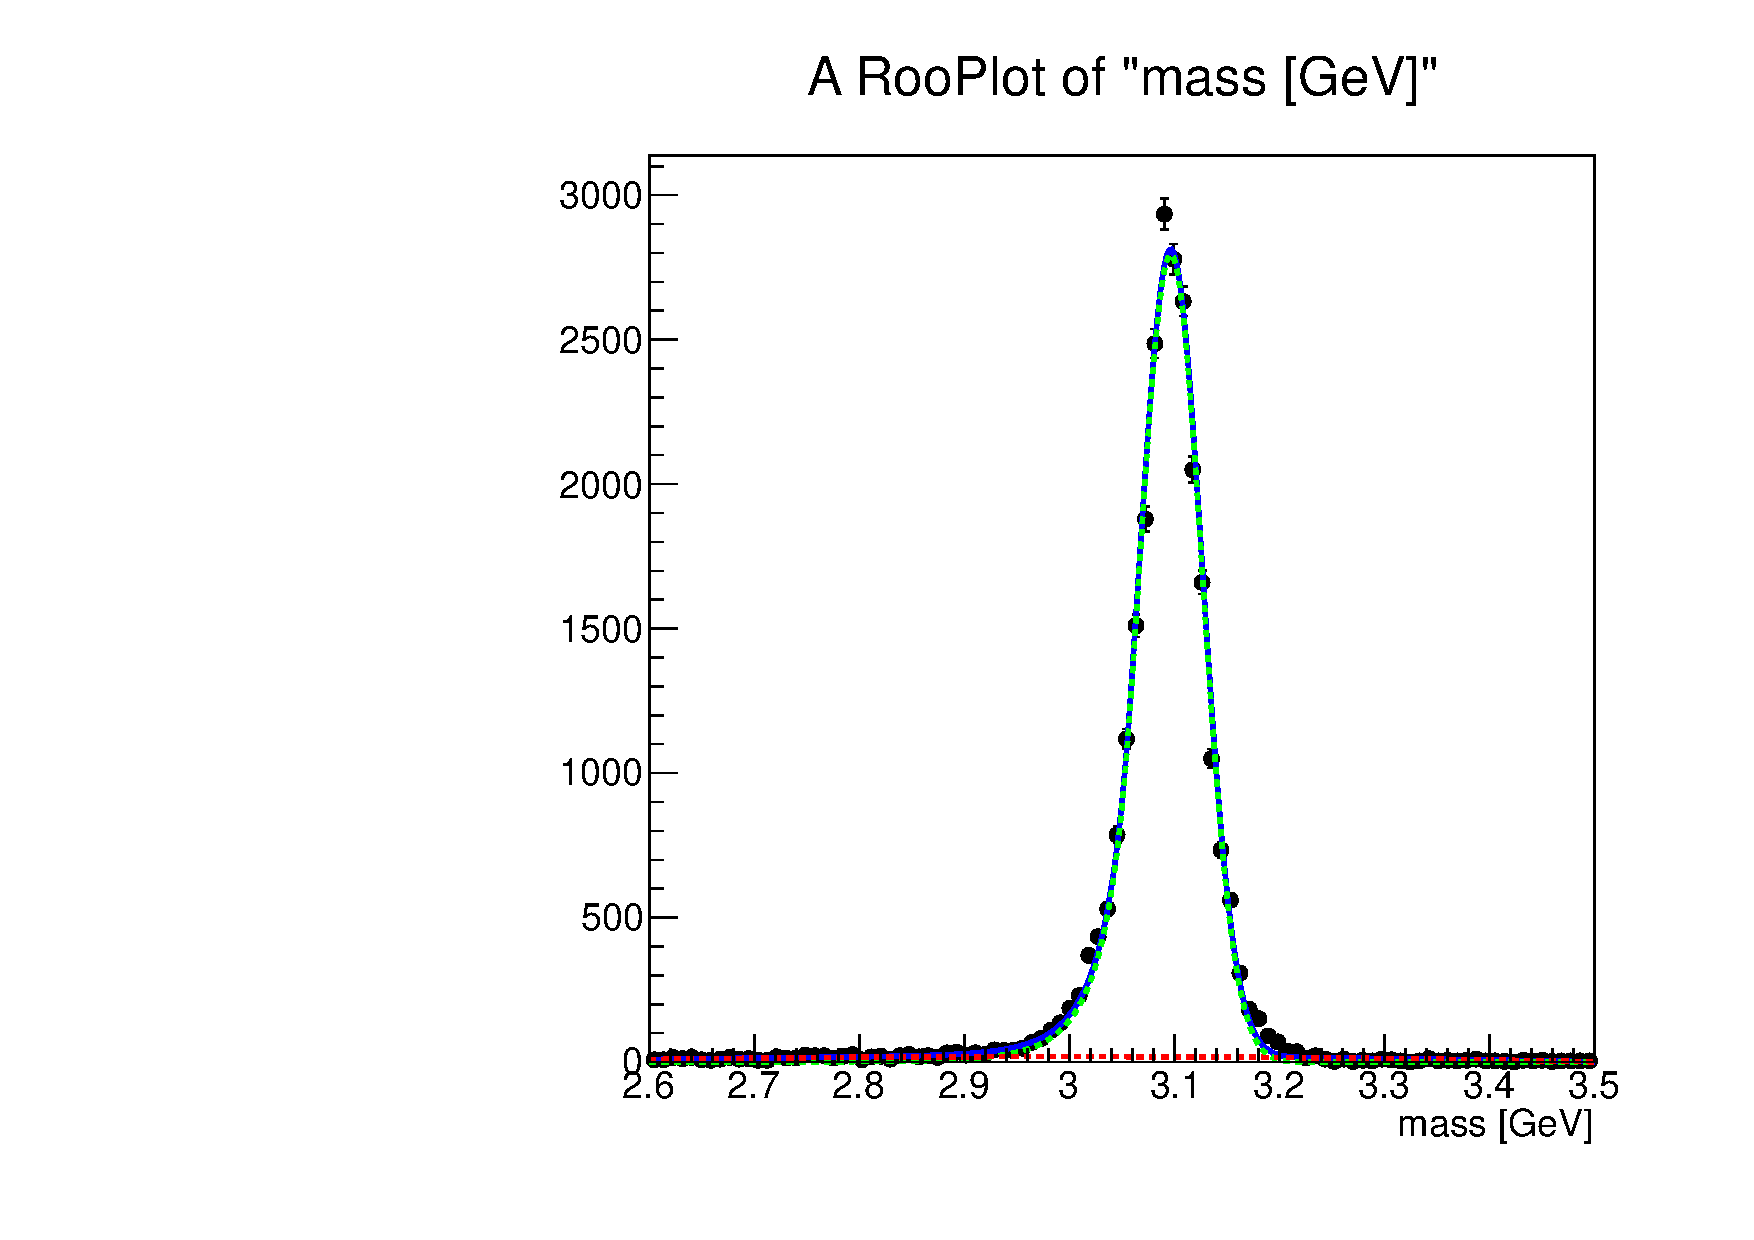
\includegraphics[width=0.25\textwidth]{../PlotsRooFitMC/croofit_id_pass_2.pdf}
    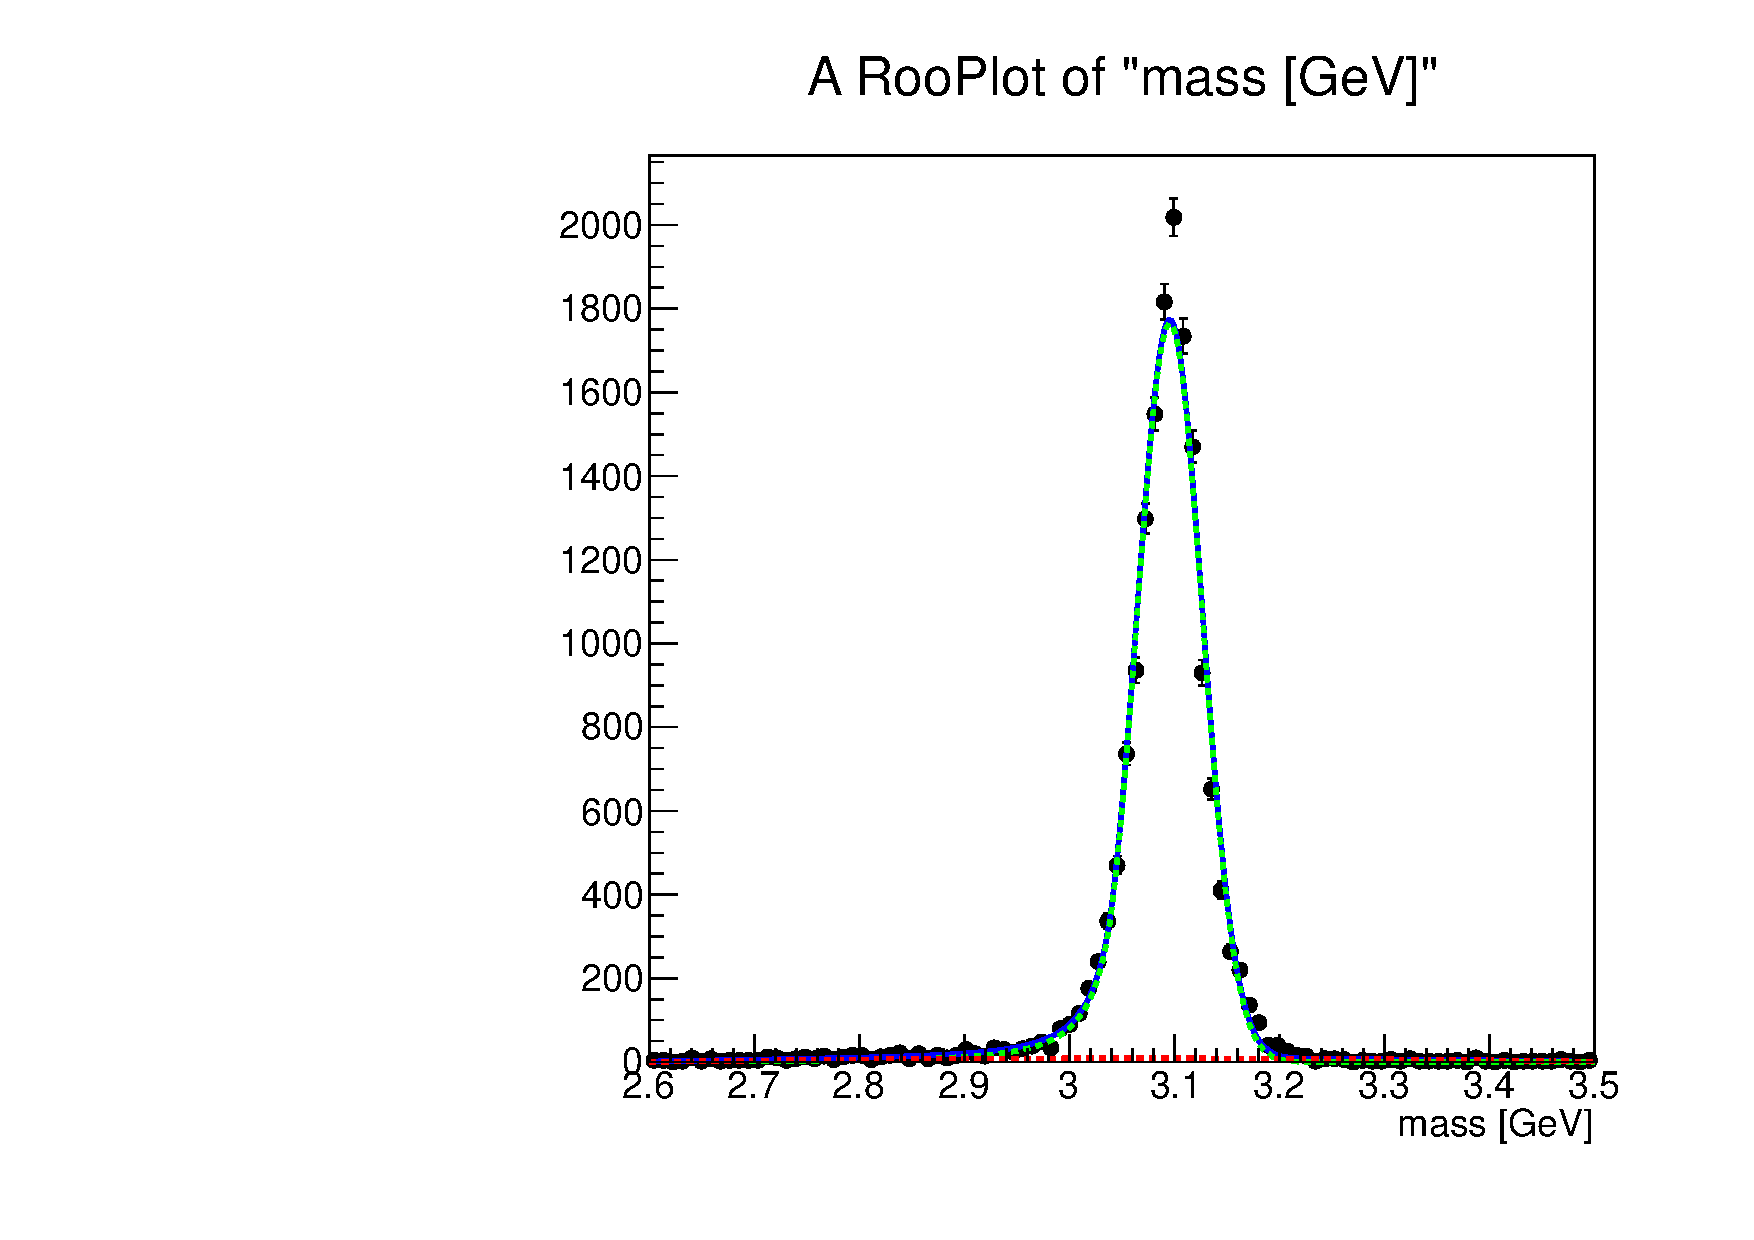
\includegraphics[width=0.25\textwidth]{../PlotsRooFitMC/croofit_id_pass_3.pdf}
    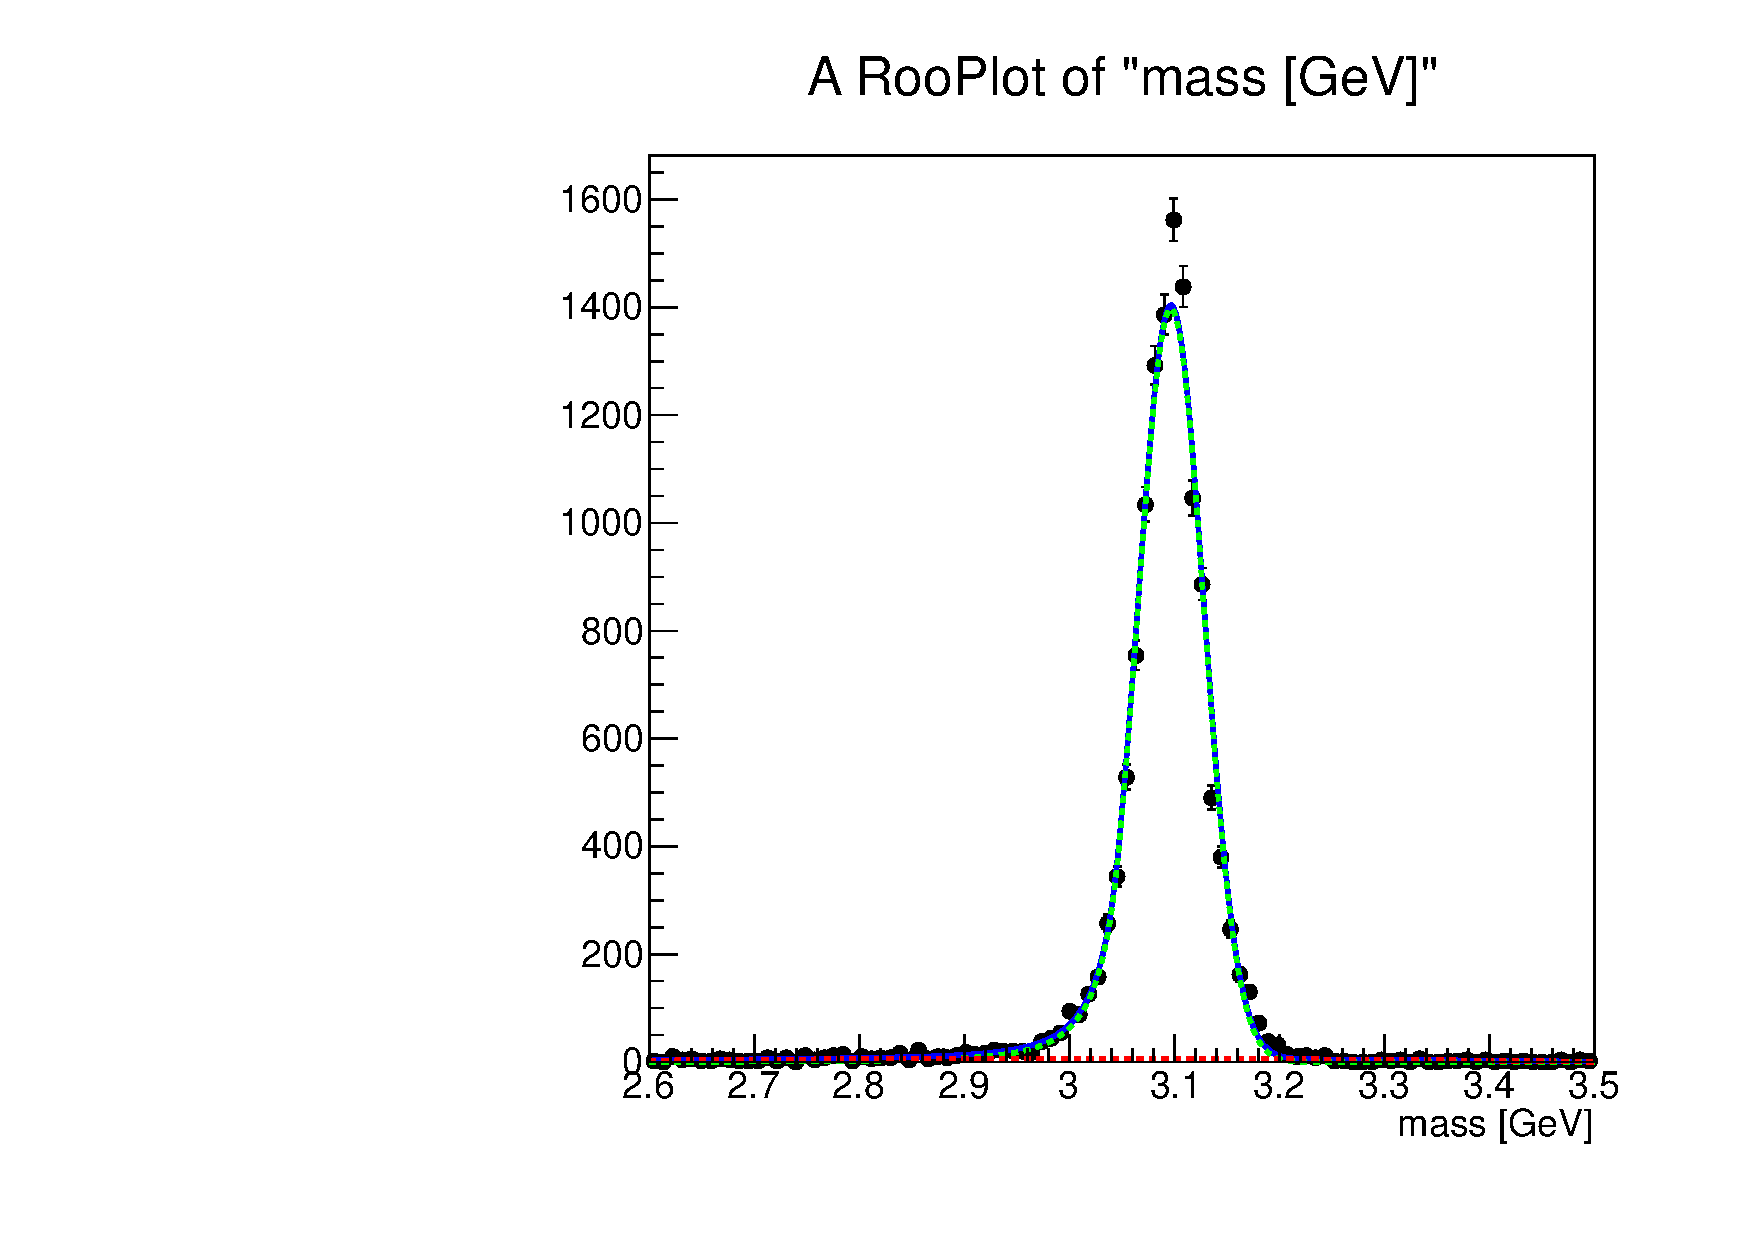
\includegraphics[width=0.25\textwidth]{../PlotsRooFitMC/croofit_id_pass_4.pdf}
    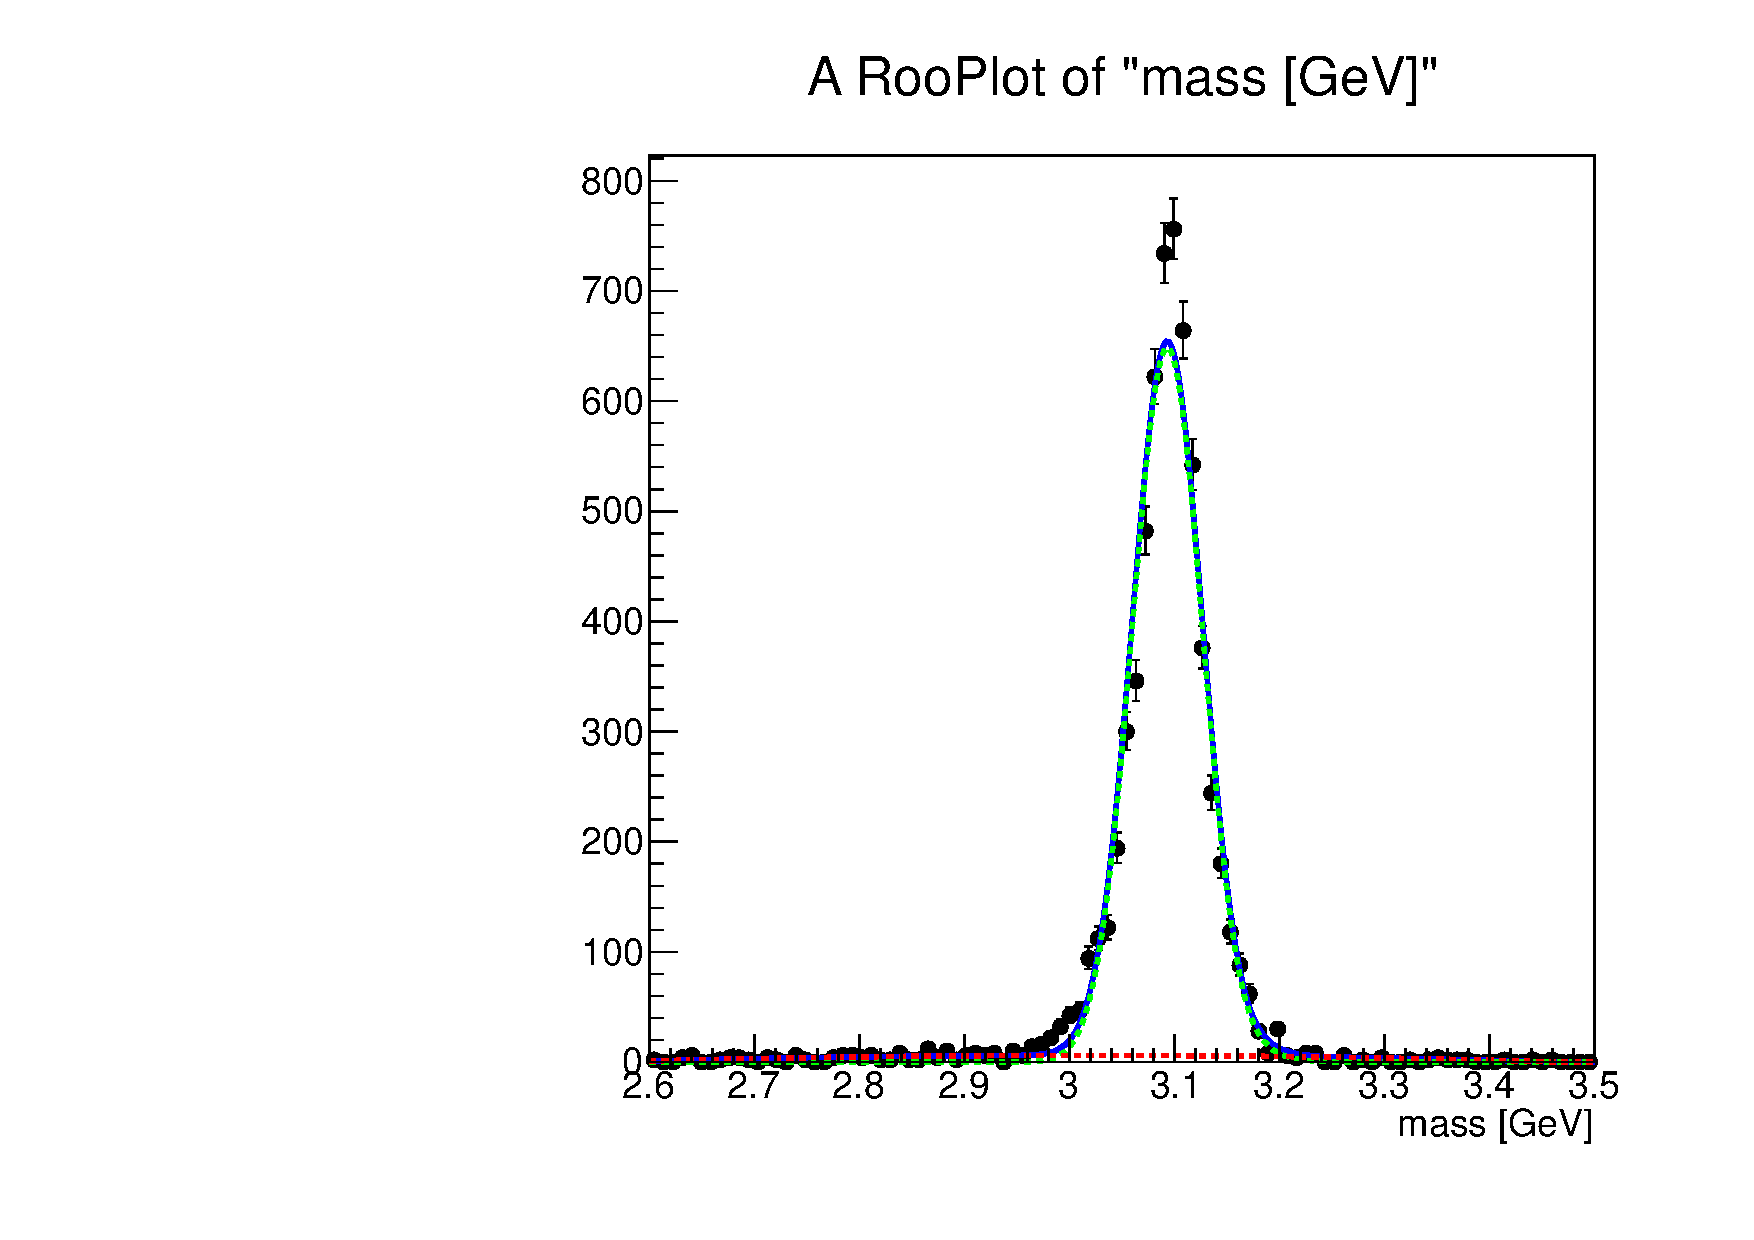
\includegraphics[width=0.25\textwidth]{../PlotsRooFitMC/croofit_id_pass_5.pdf}
    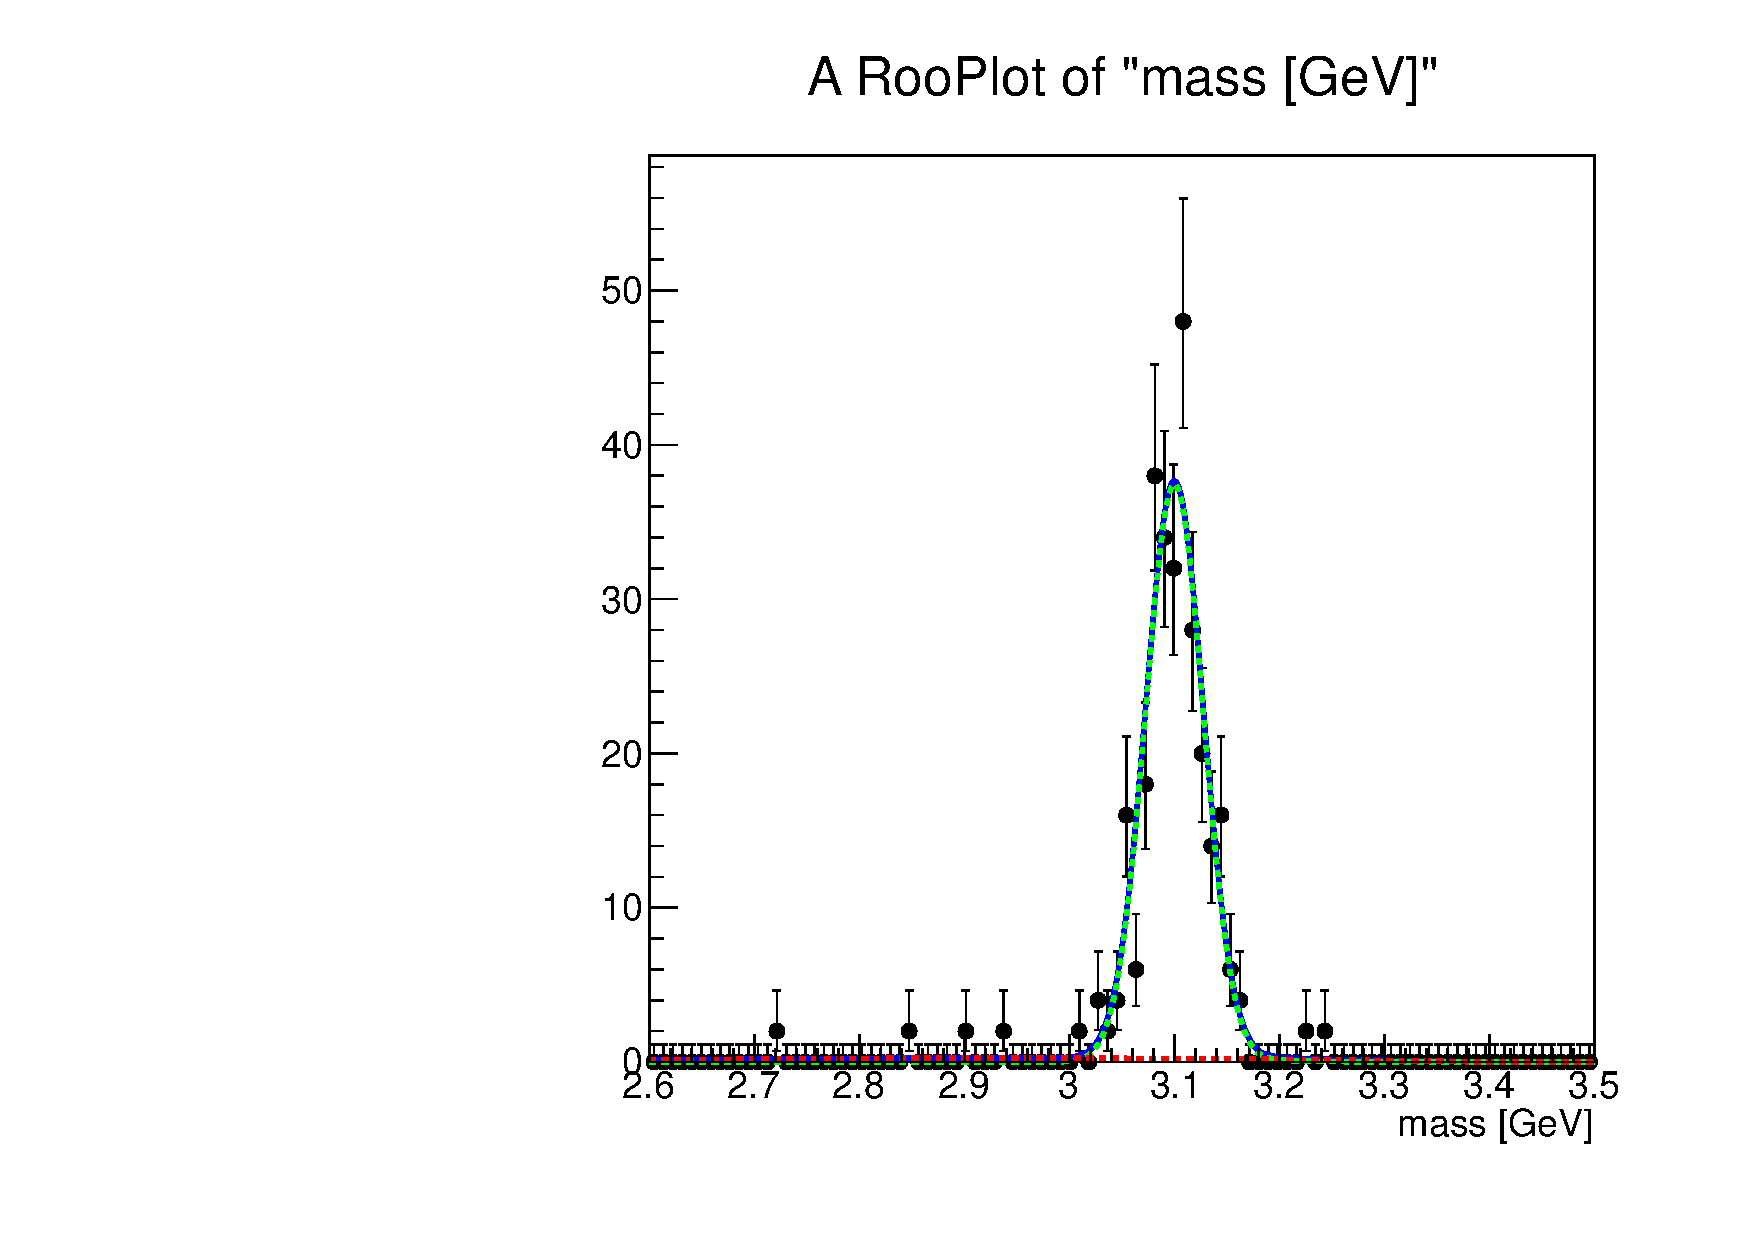
\includegraphics[width=0.25\textwidth]{../PlotsRooFitMC/croofit_id_pass_6.pdf}
    \caption{MC Results muonID studies for passing probes, muon transverse momenta
    $\rm p_{t}$ (GeV/c)= {0.0-1.5}, {1.5-3.0}, {3.0-4.5}, {4.5-6.0}, 
    {6.0-9.0}, {9.0-20.0}, {20.0-30.0}}
   % \label{simulationfigure}
\end{figure}

\begin{figure}
    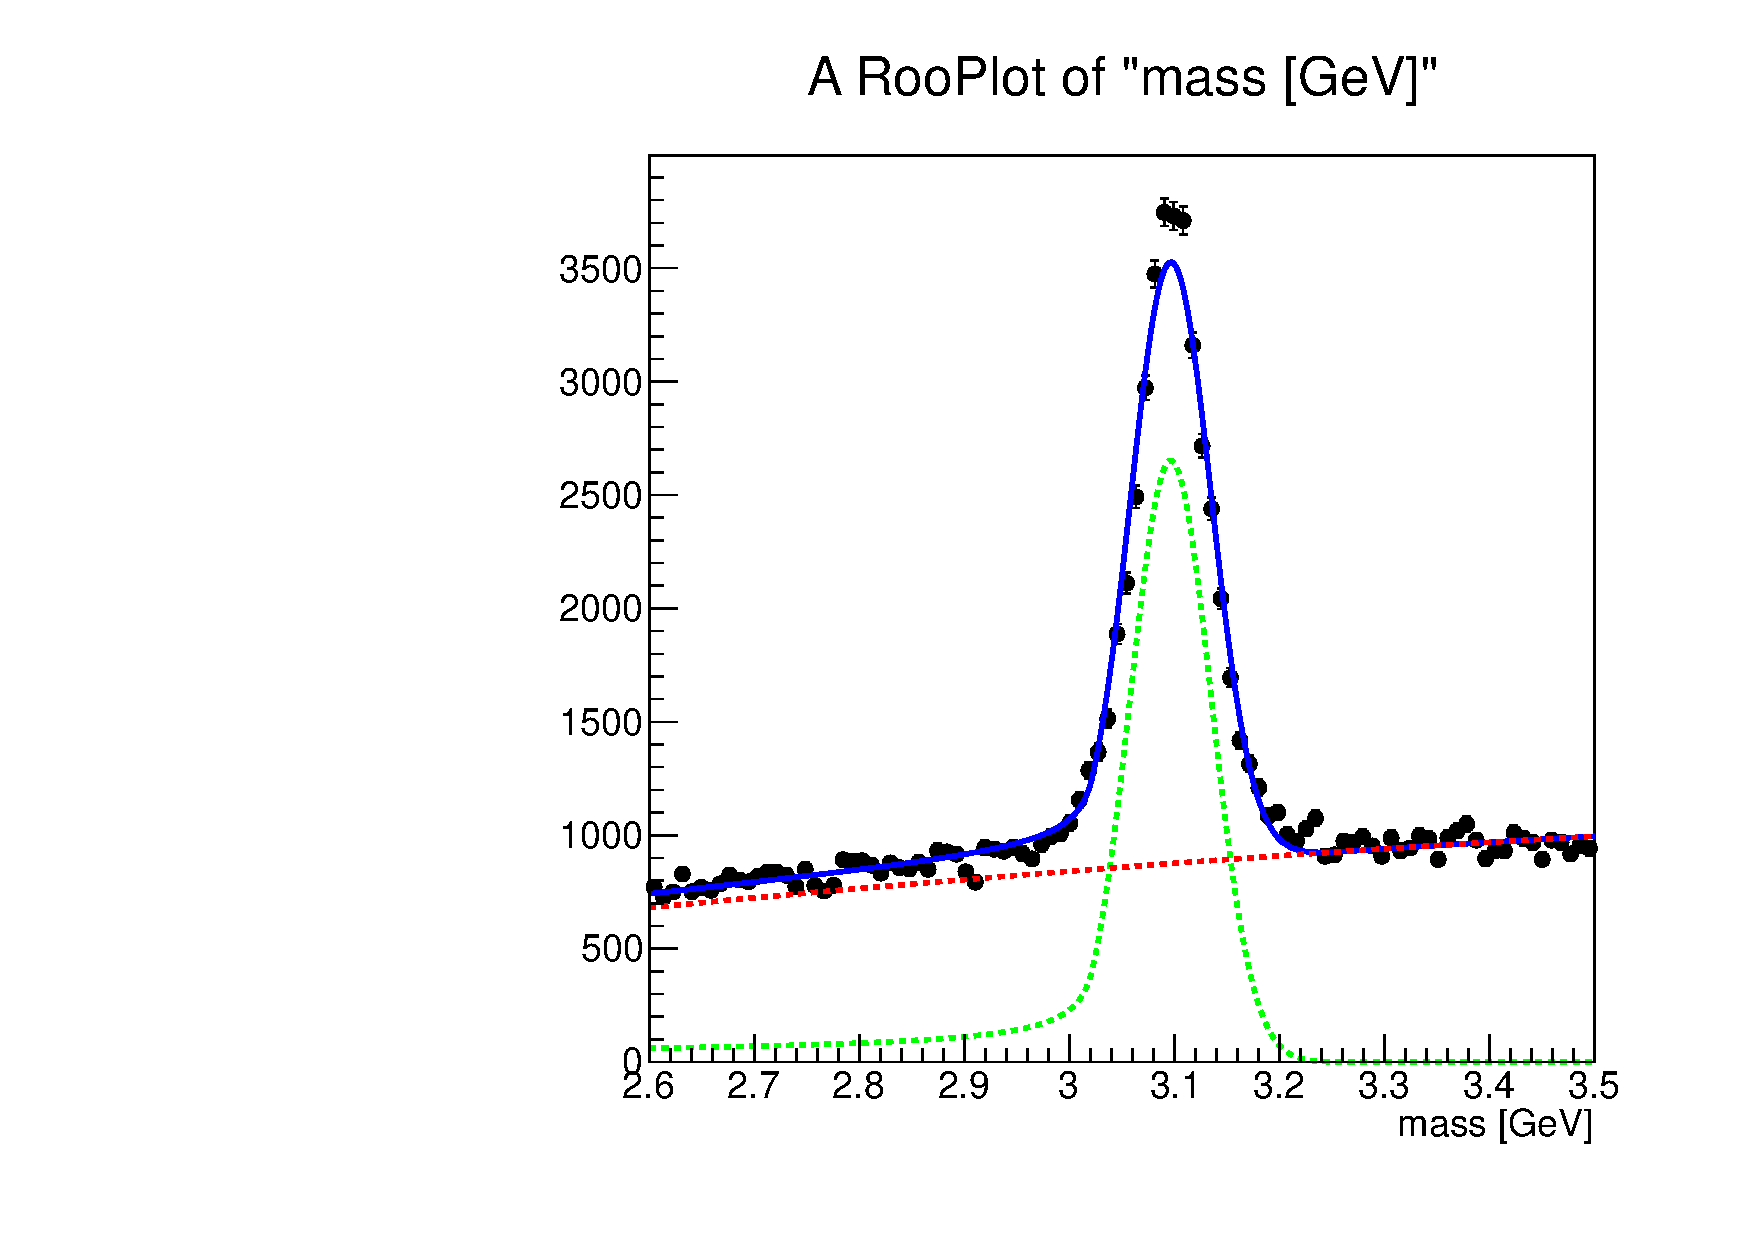
\includegraphics[width=0.25\textwidth]{../PlotsRooFitMC/croofit_id_fail_0.pdf}
    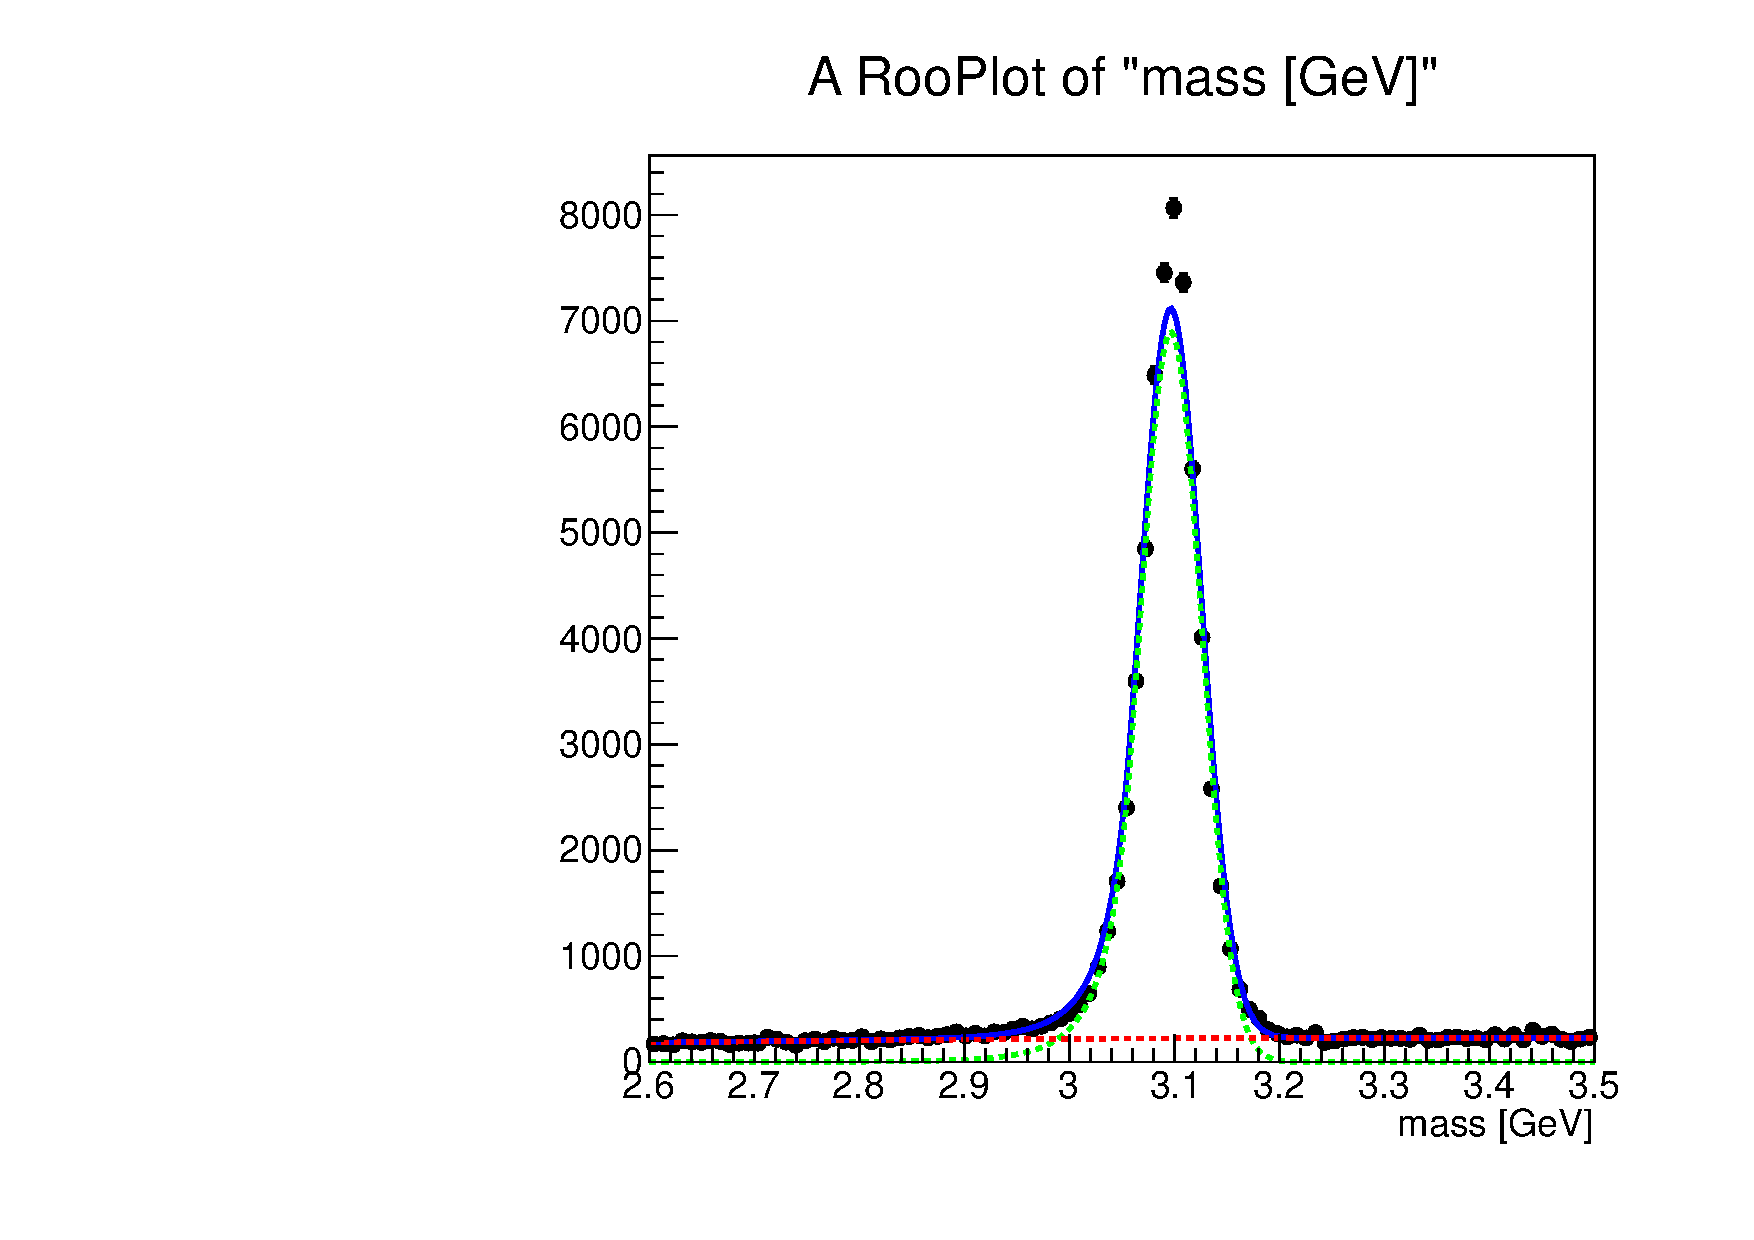
\includegraphics[width=0.25\textwidth]{../PlotsRooFitMC/croofit_id_fail_1.pdf}
    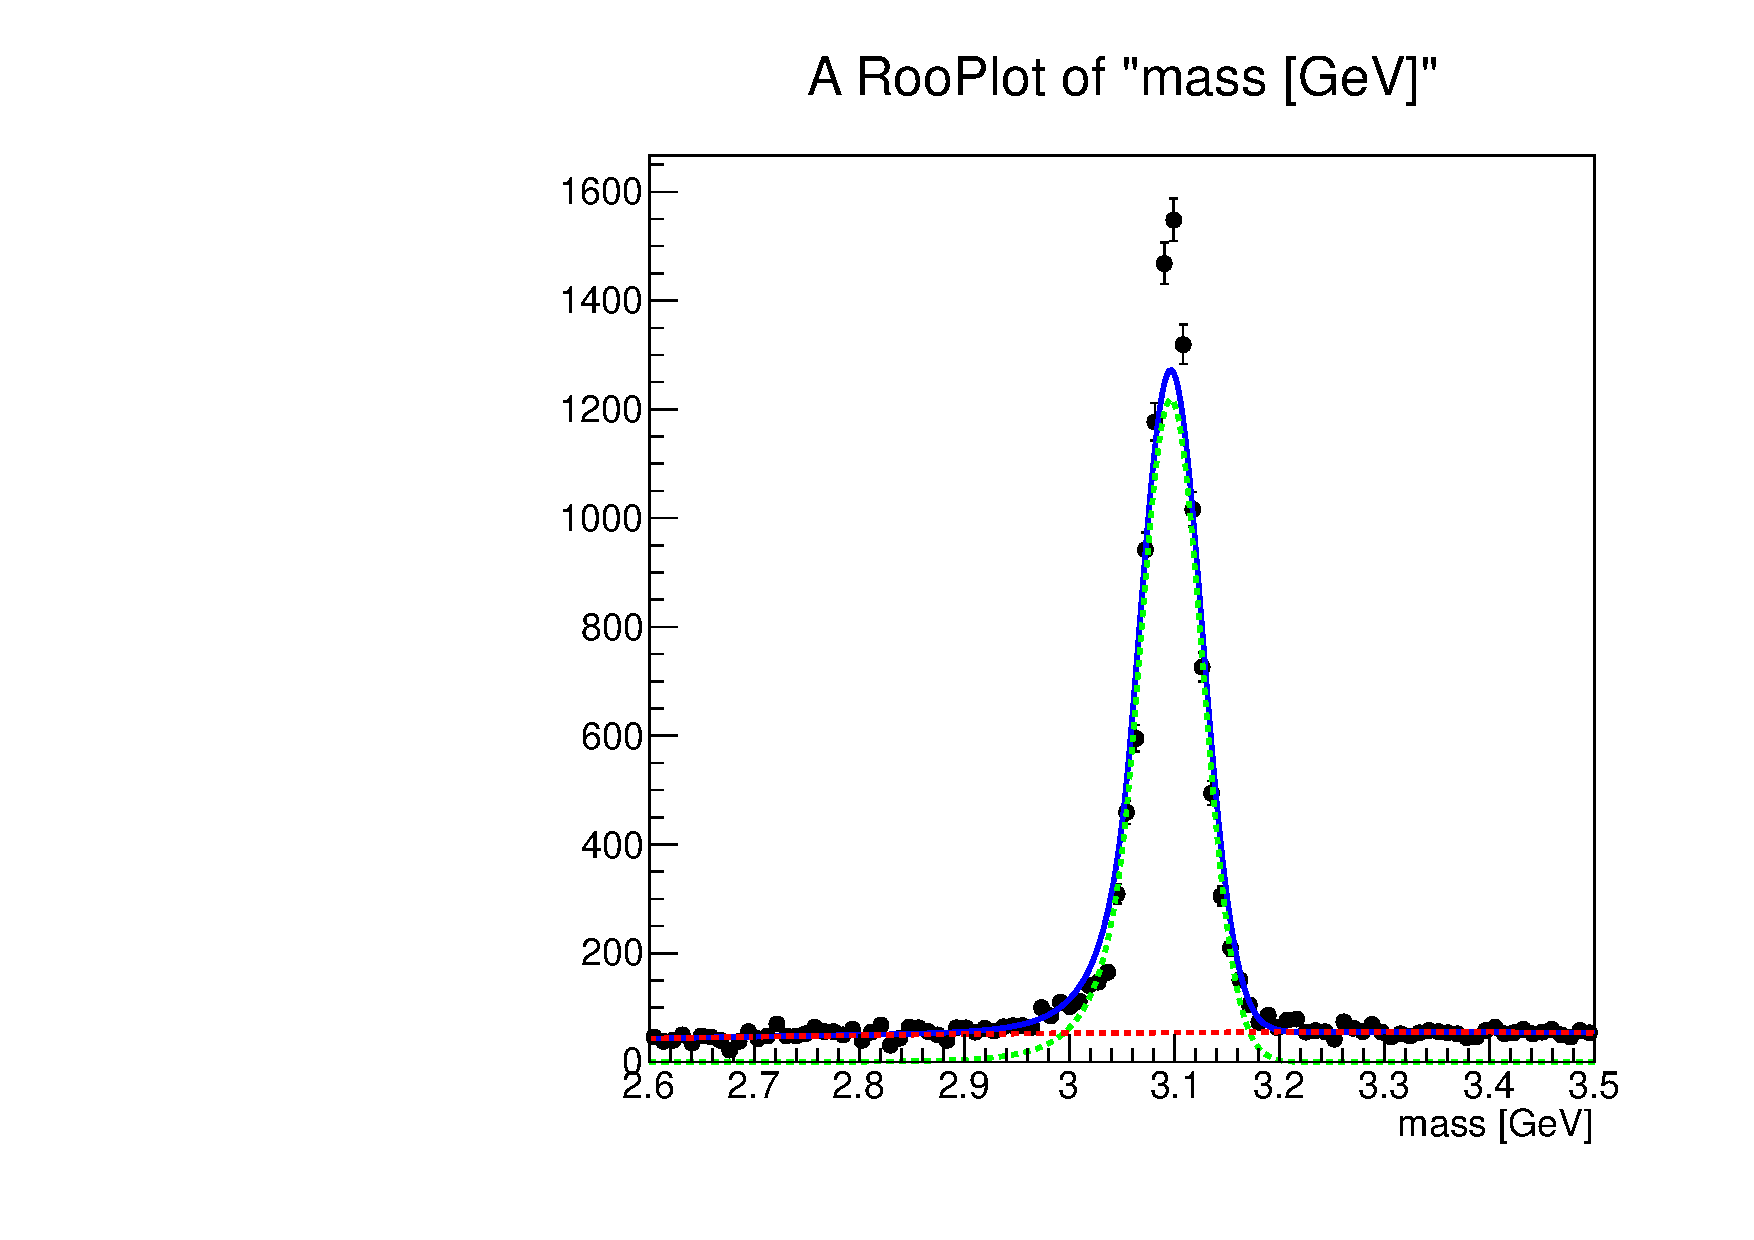
\includegraphics[width=0.25\textwidth]{../PlotsRooFitMC/croofit_id_fail_2.pdf}
    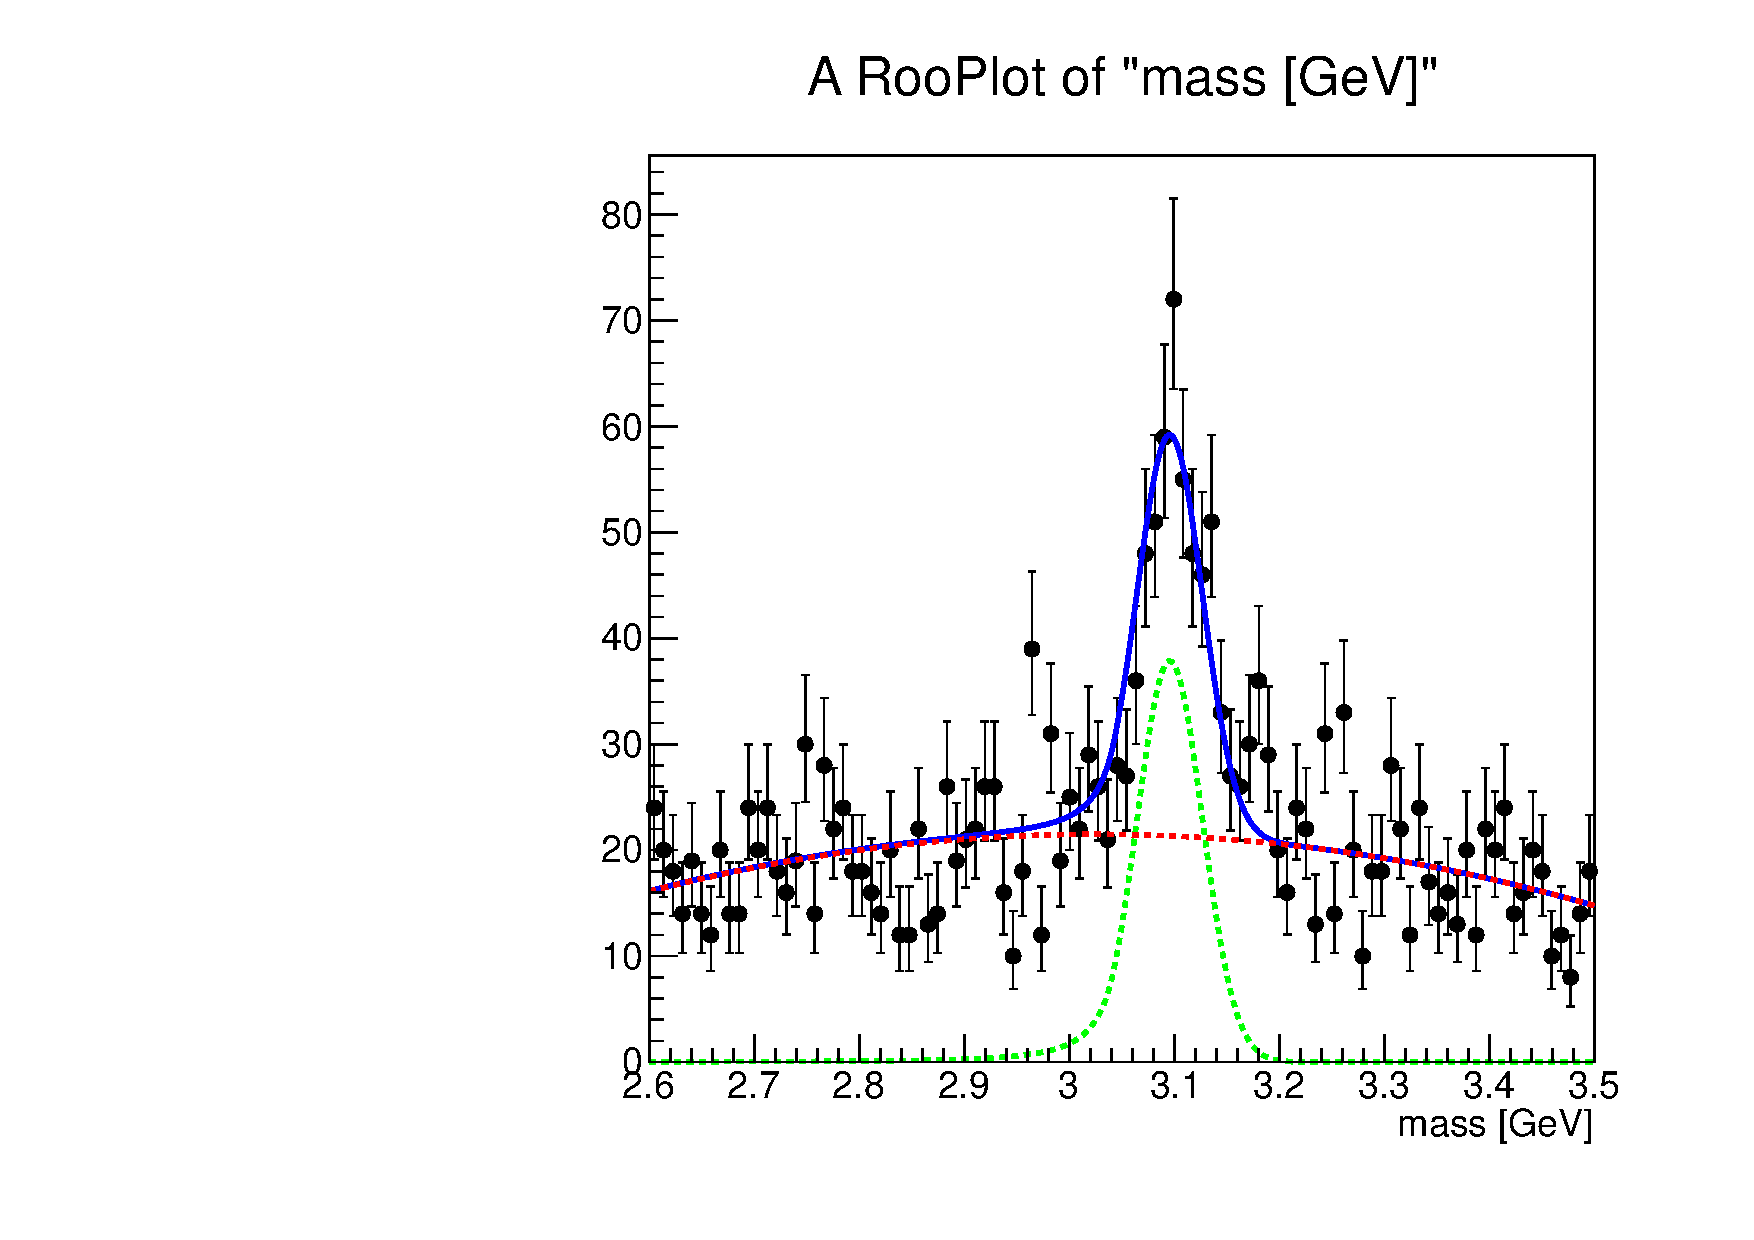
\includegraphics[width=0.25\textwidth]{../PlotsRooFitMC/croofit_id_fail_3.pdf}
    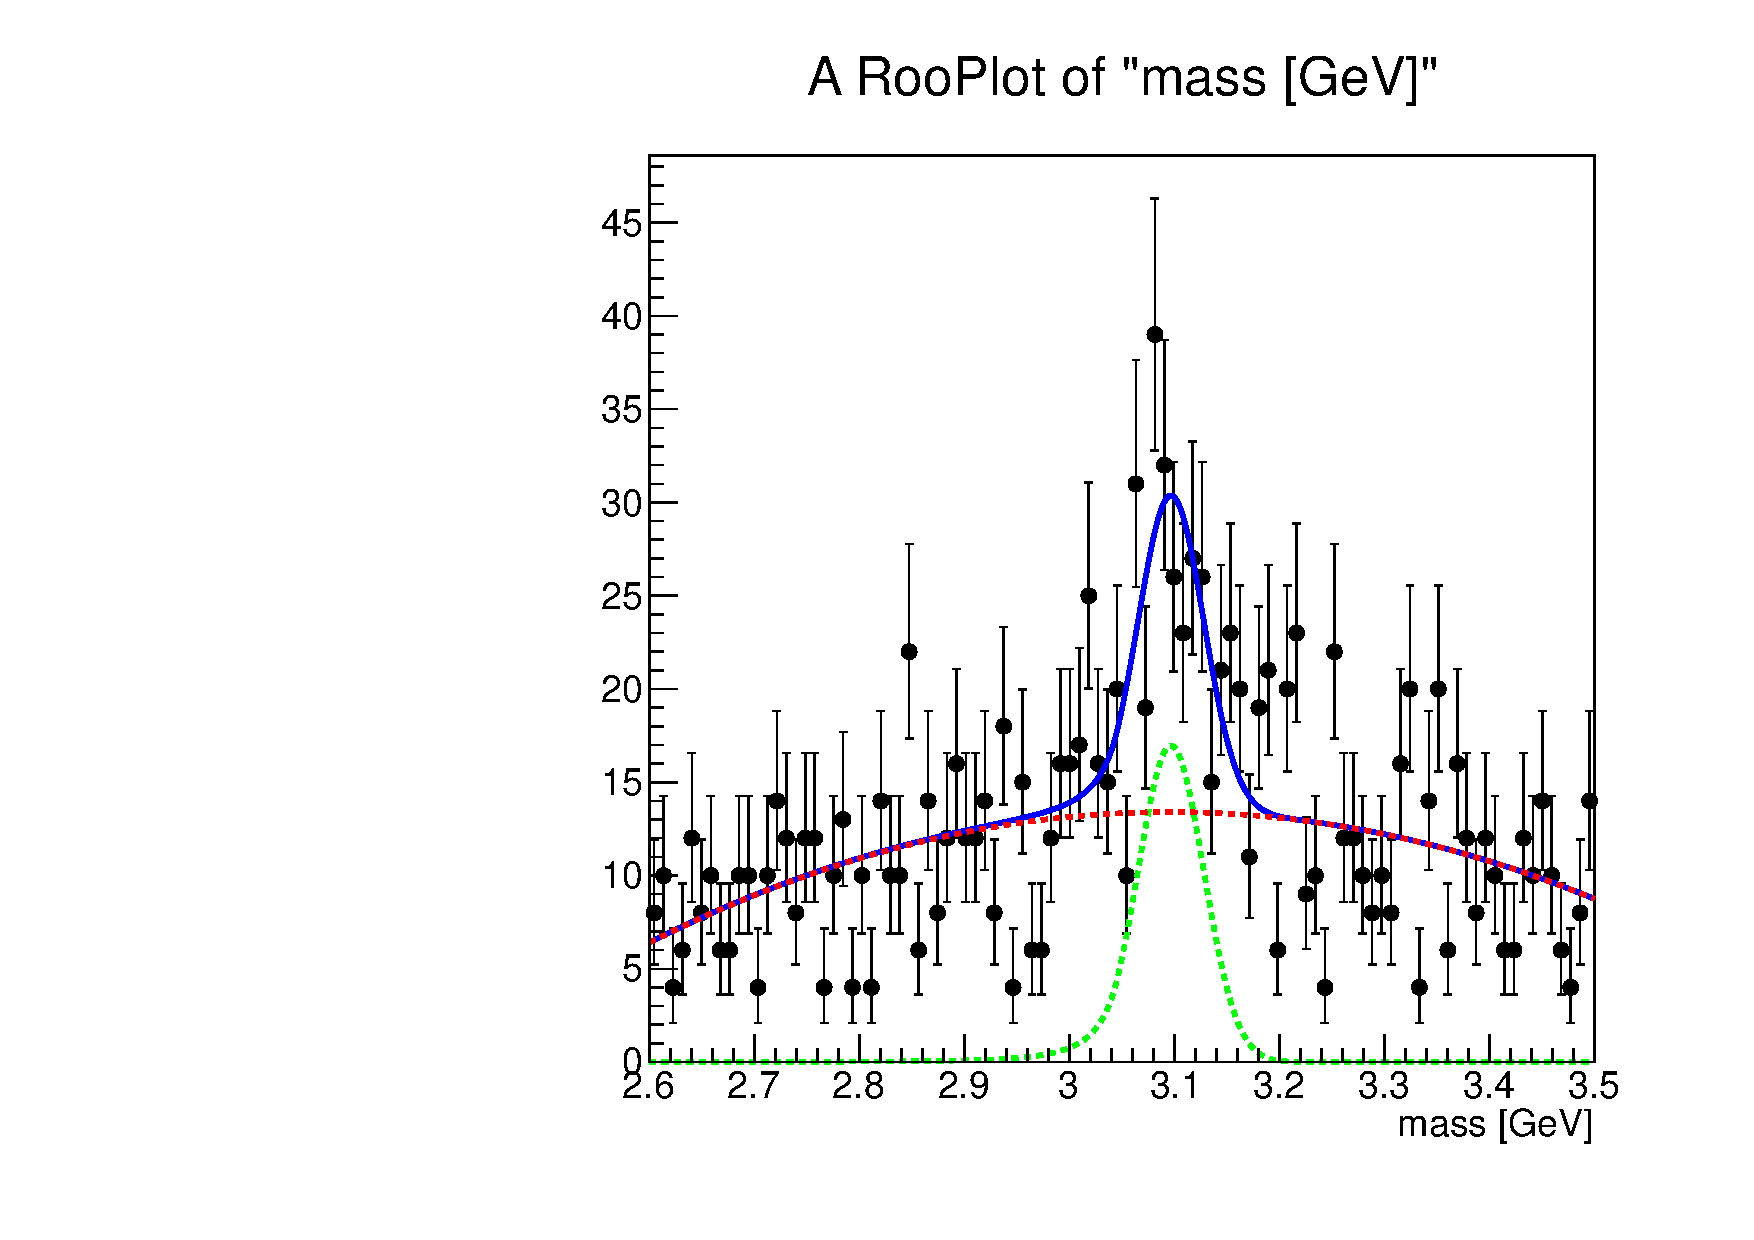
\includegraphics[width=0.25\textwidth]{../PlotsRooFitMC/croofit_id_fail_4.pdf}
    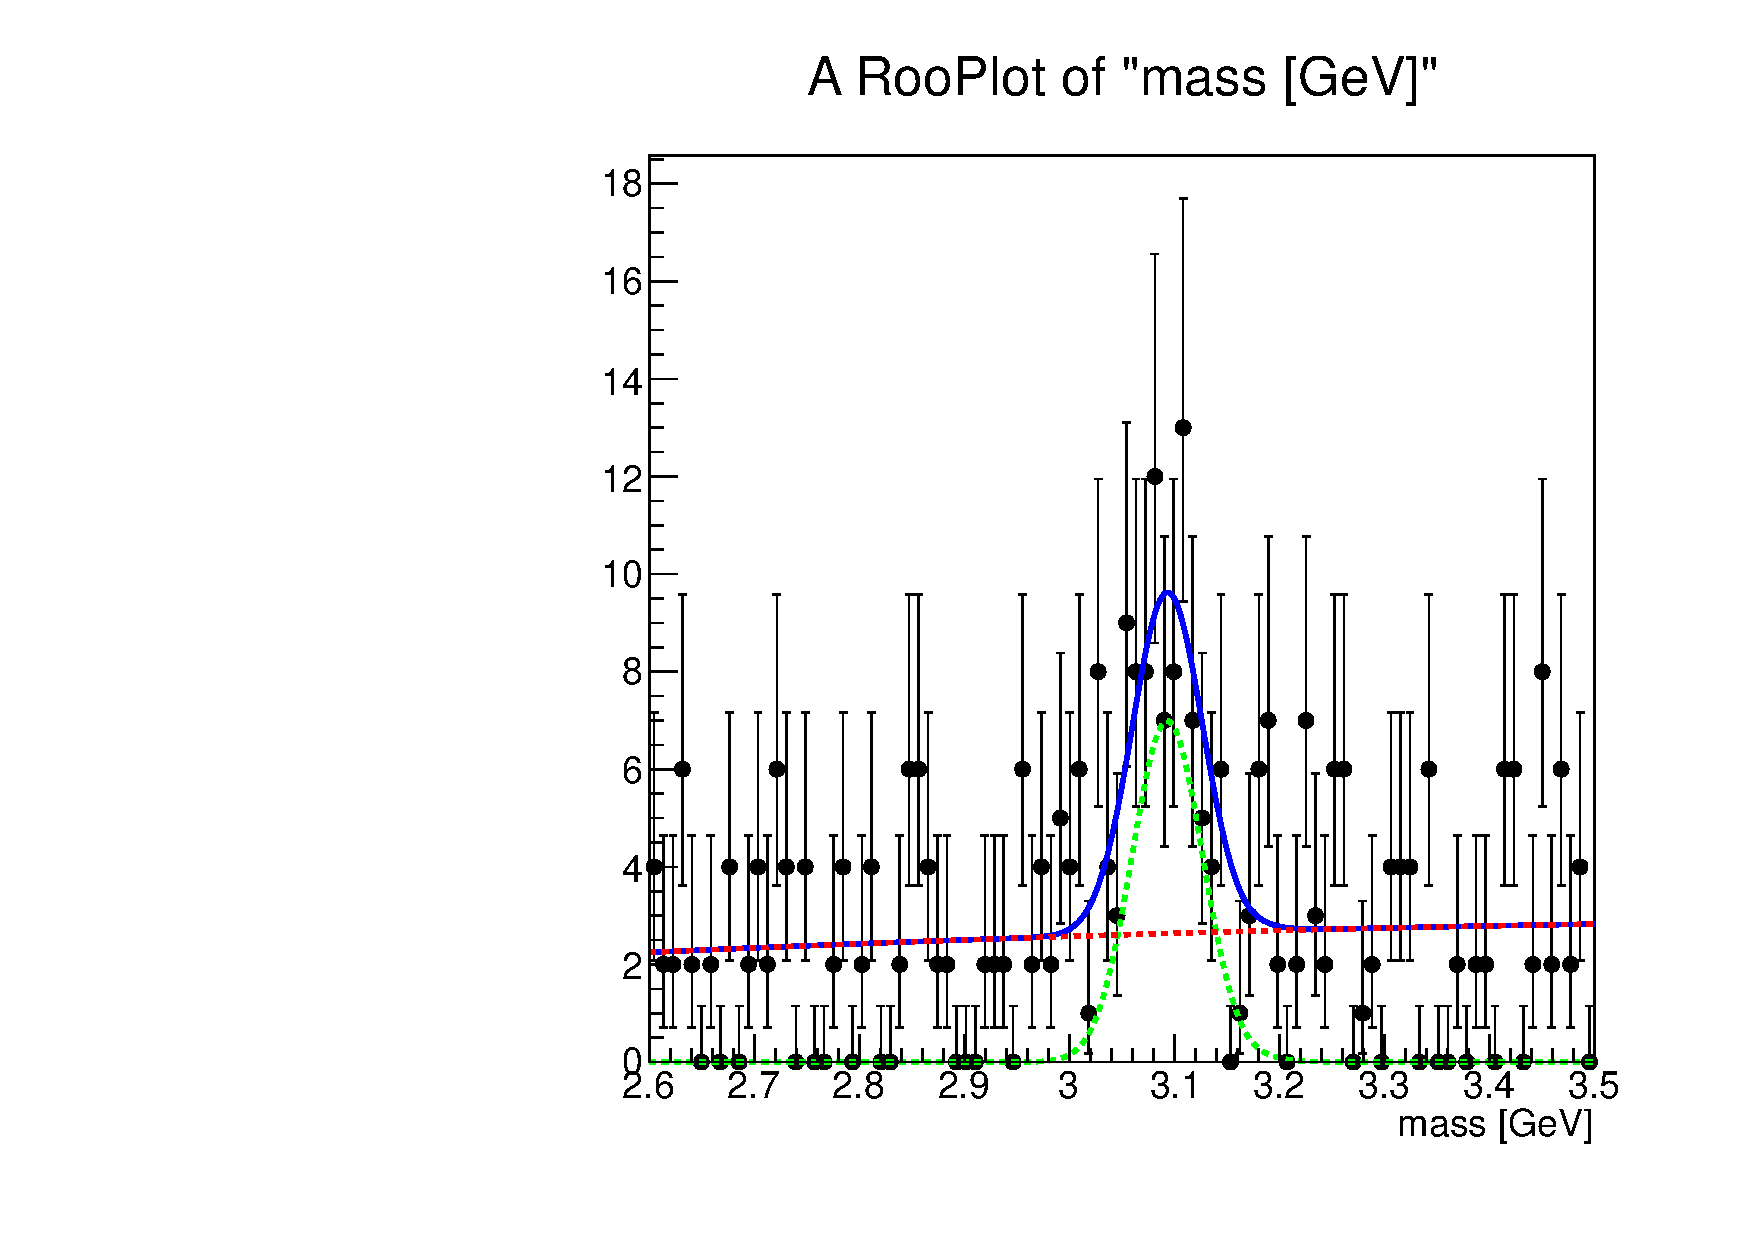
\includegraphics[width=0.25\textwidth]{../PlotsRooFitMC/croofit_id_fail_5.pdf}
    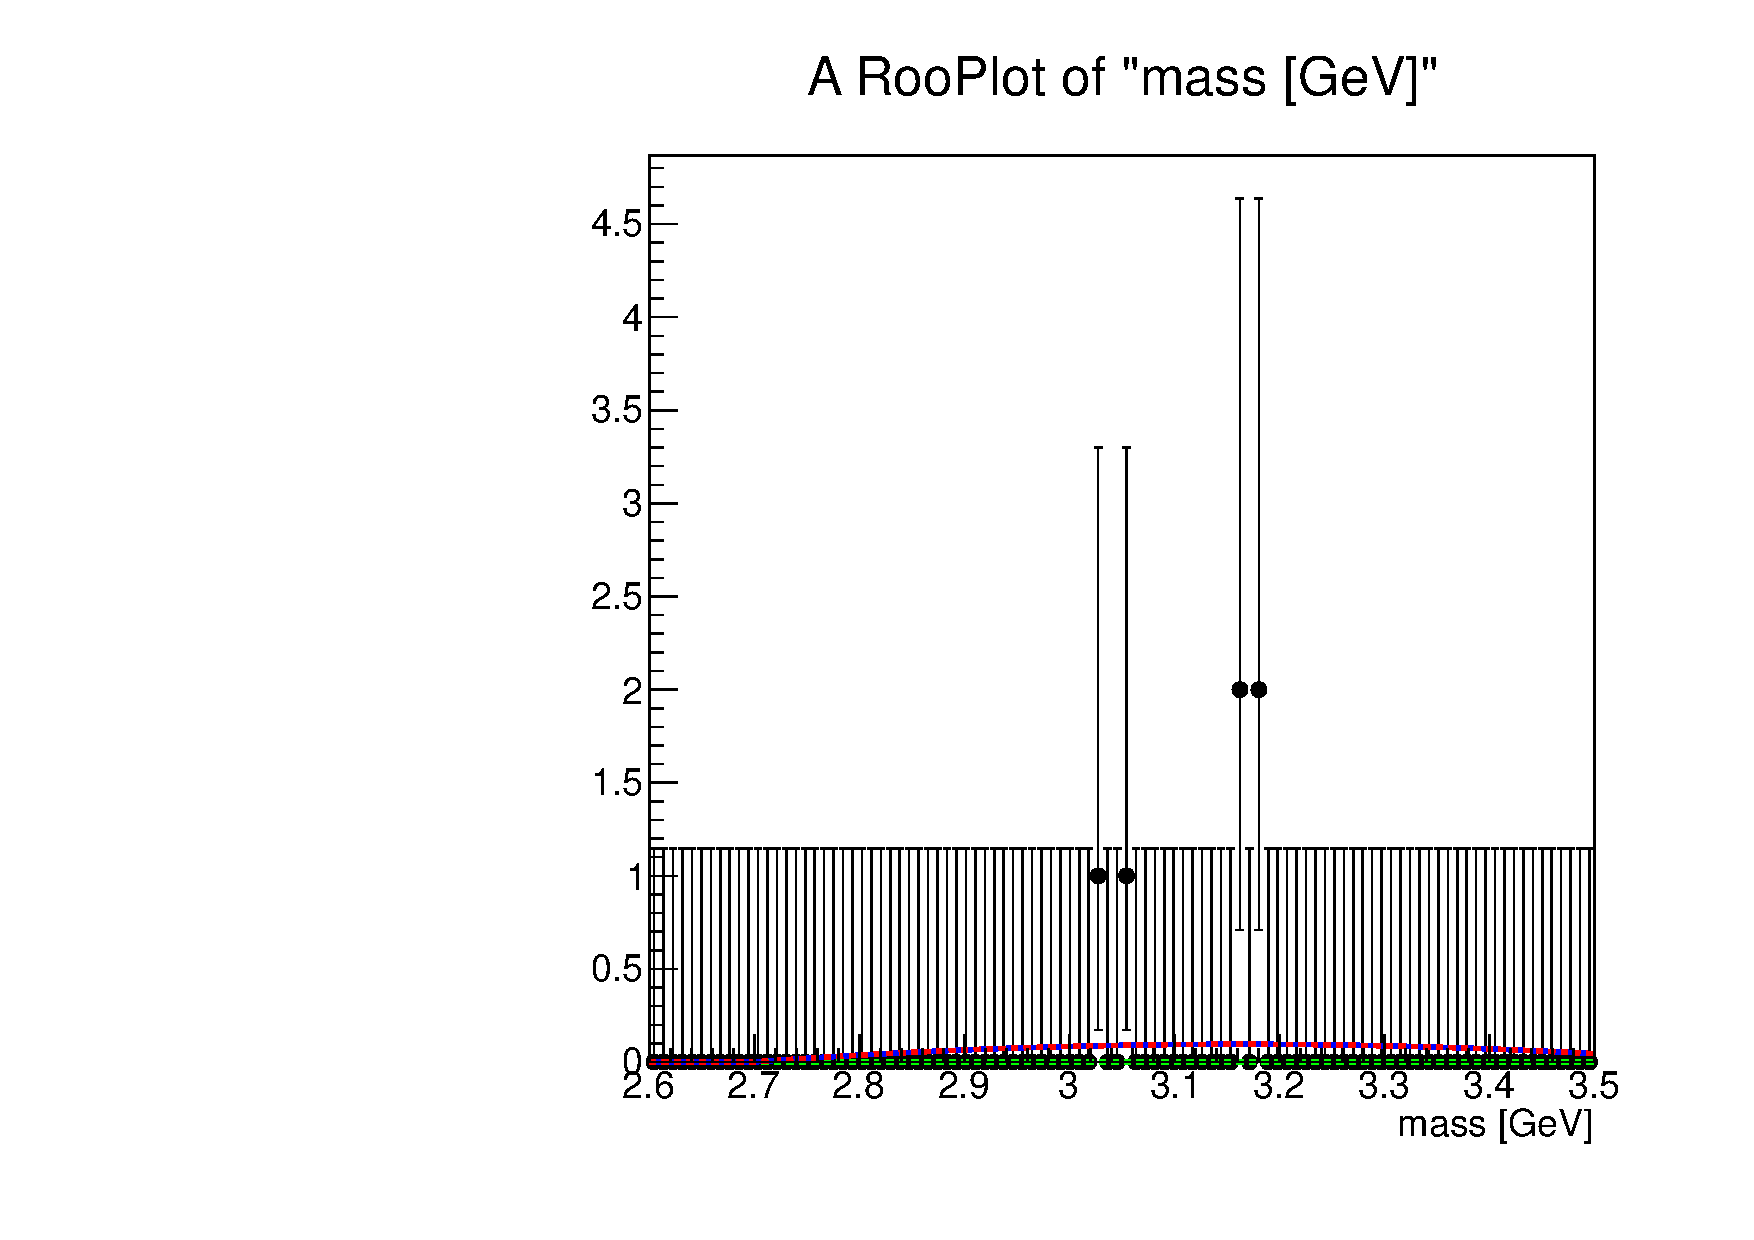
\includegraphics[width=0.25\textwidth]{../PlotsRooFitMC/croofit_id_fail_6.pdf}
    \caption{MC Results muonID studies for failing probes, muon transverse momenta
    $\rm p_{t}$ (GeV/c)= {0.0-1.5}, {1.5-3.0}, {3.0-4.5}, {4.5-6.0}, 
    {6.0-9.0}, {9.0-20.0}, {20.0-30.0}}
   % \label{simulationfigure}
\end{figure}

\begin{figure}
    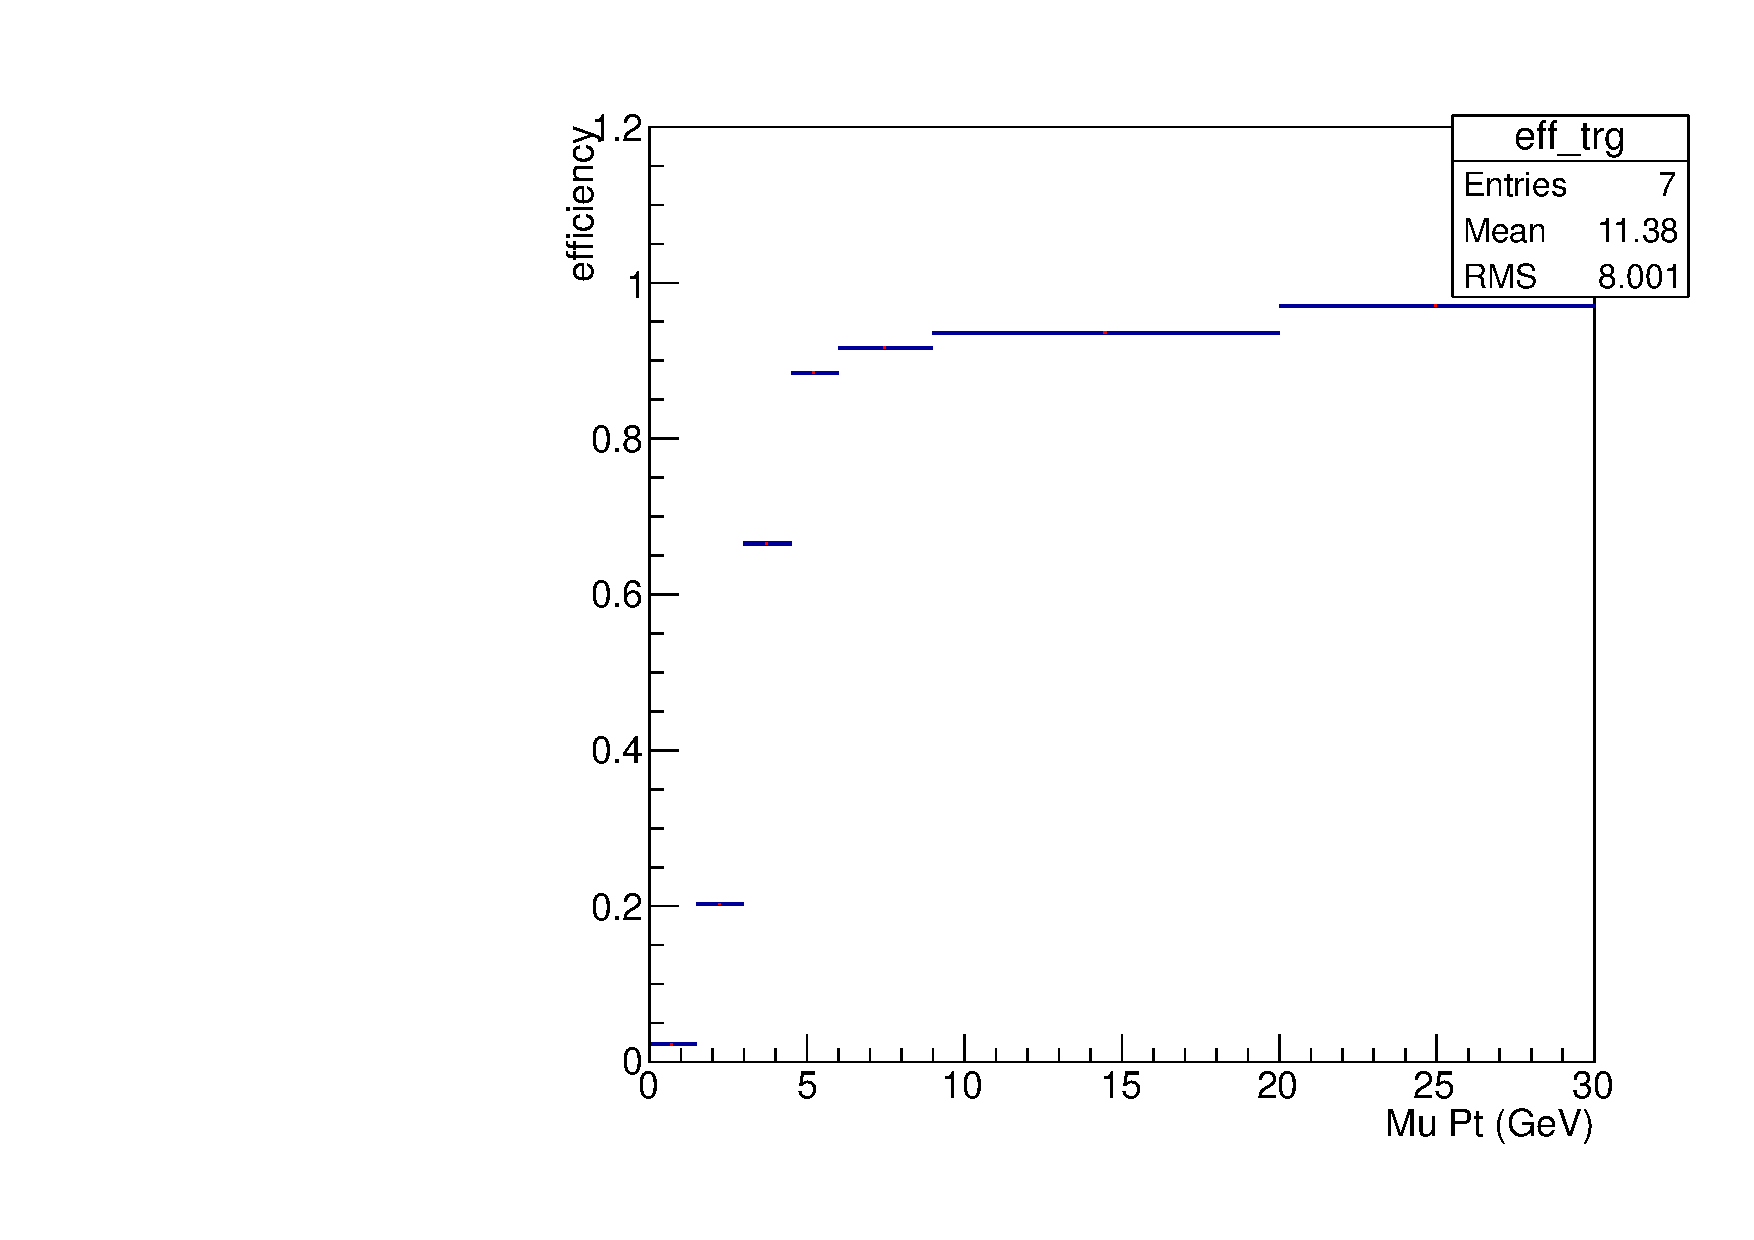
\includegraphics[width=0.25\textwidth]{../PlotsRooFitMC/eff_trg.pdf}
    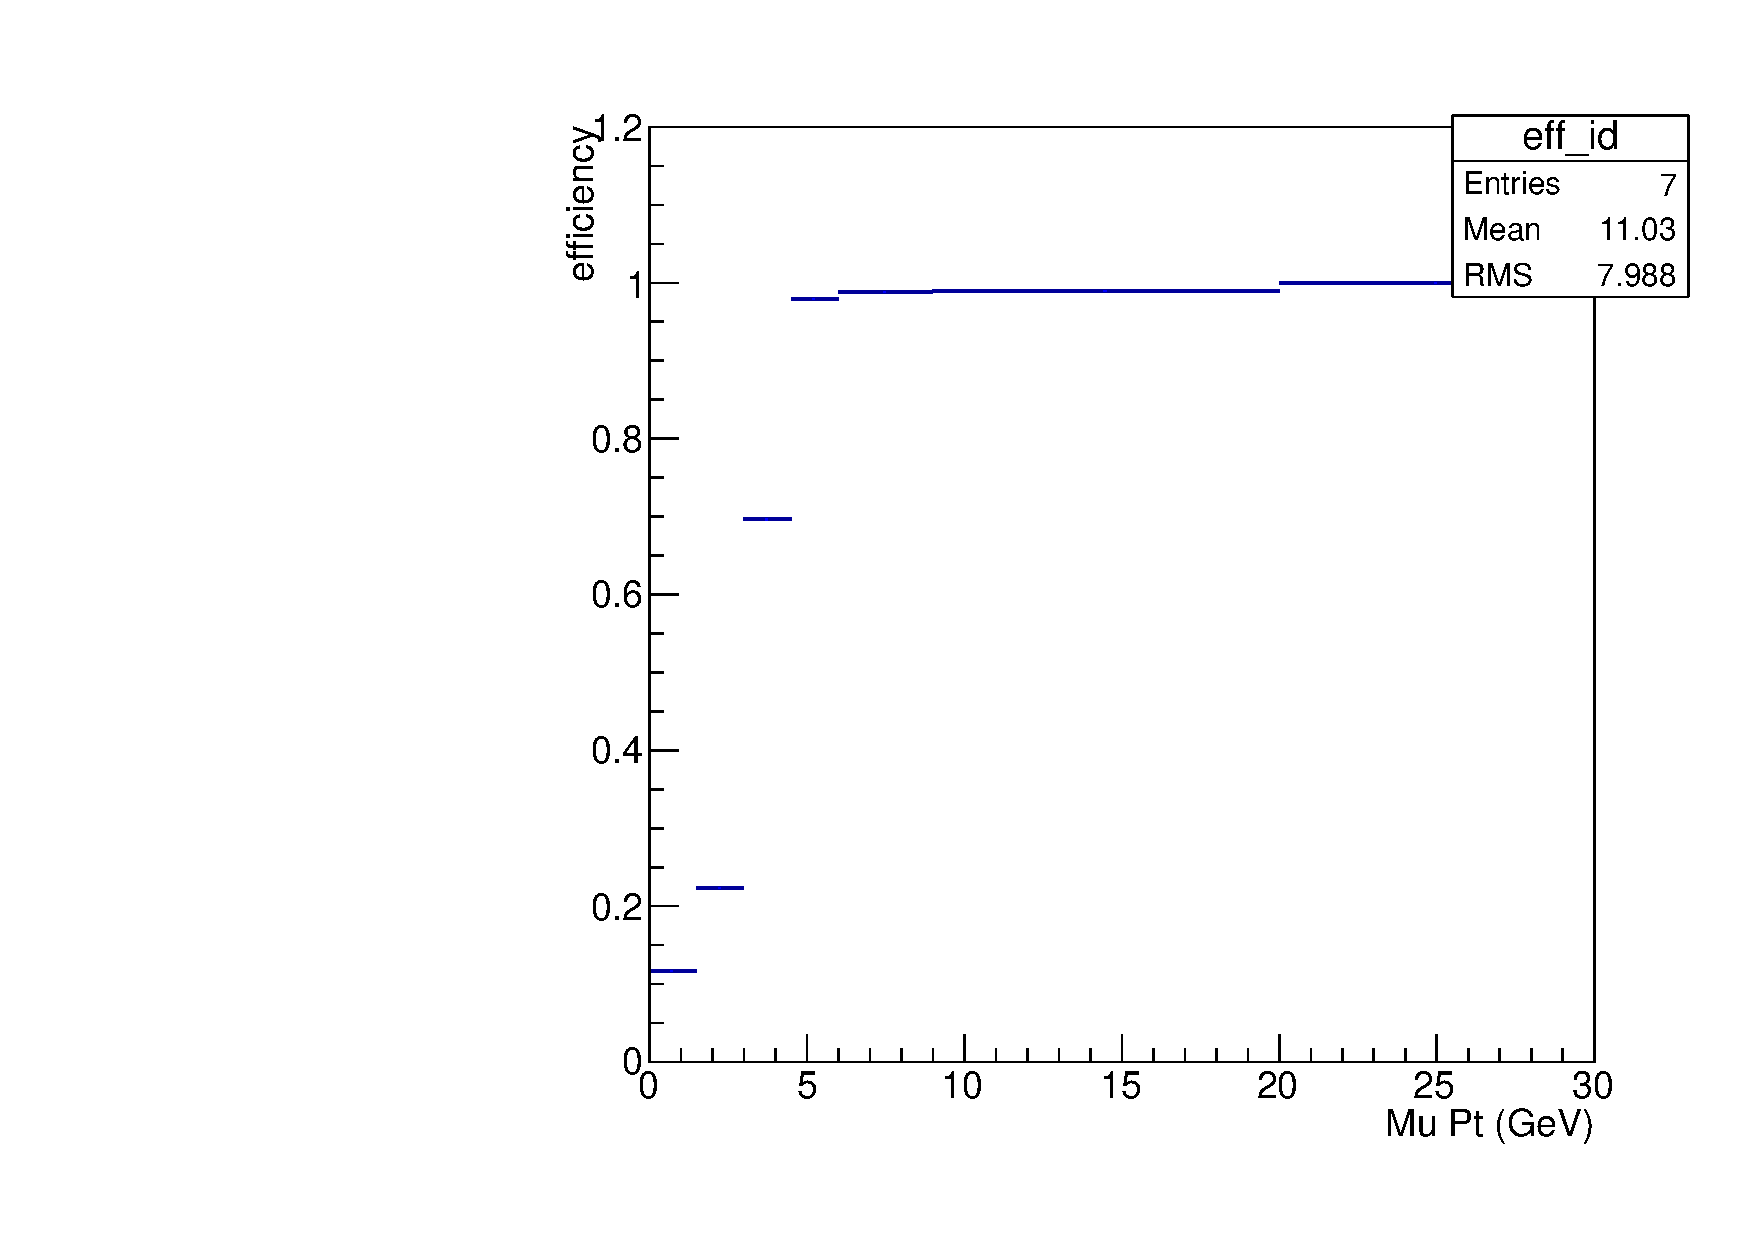
\includegraphics[width=0.25\textwidth]{../PlotsRooFitMC/eff_id.pdf}
    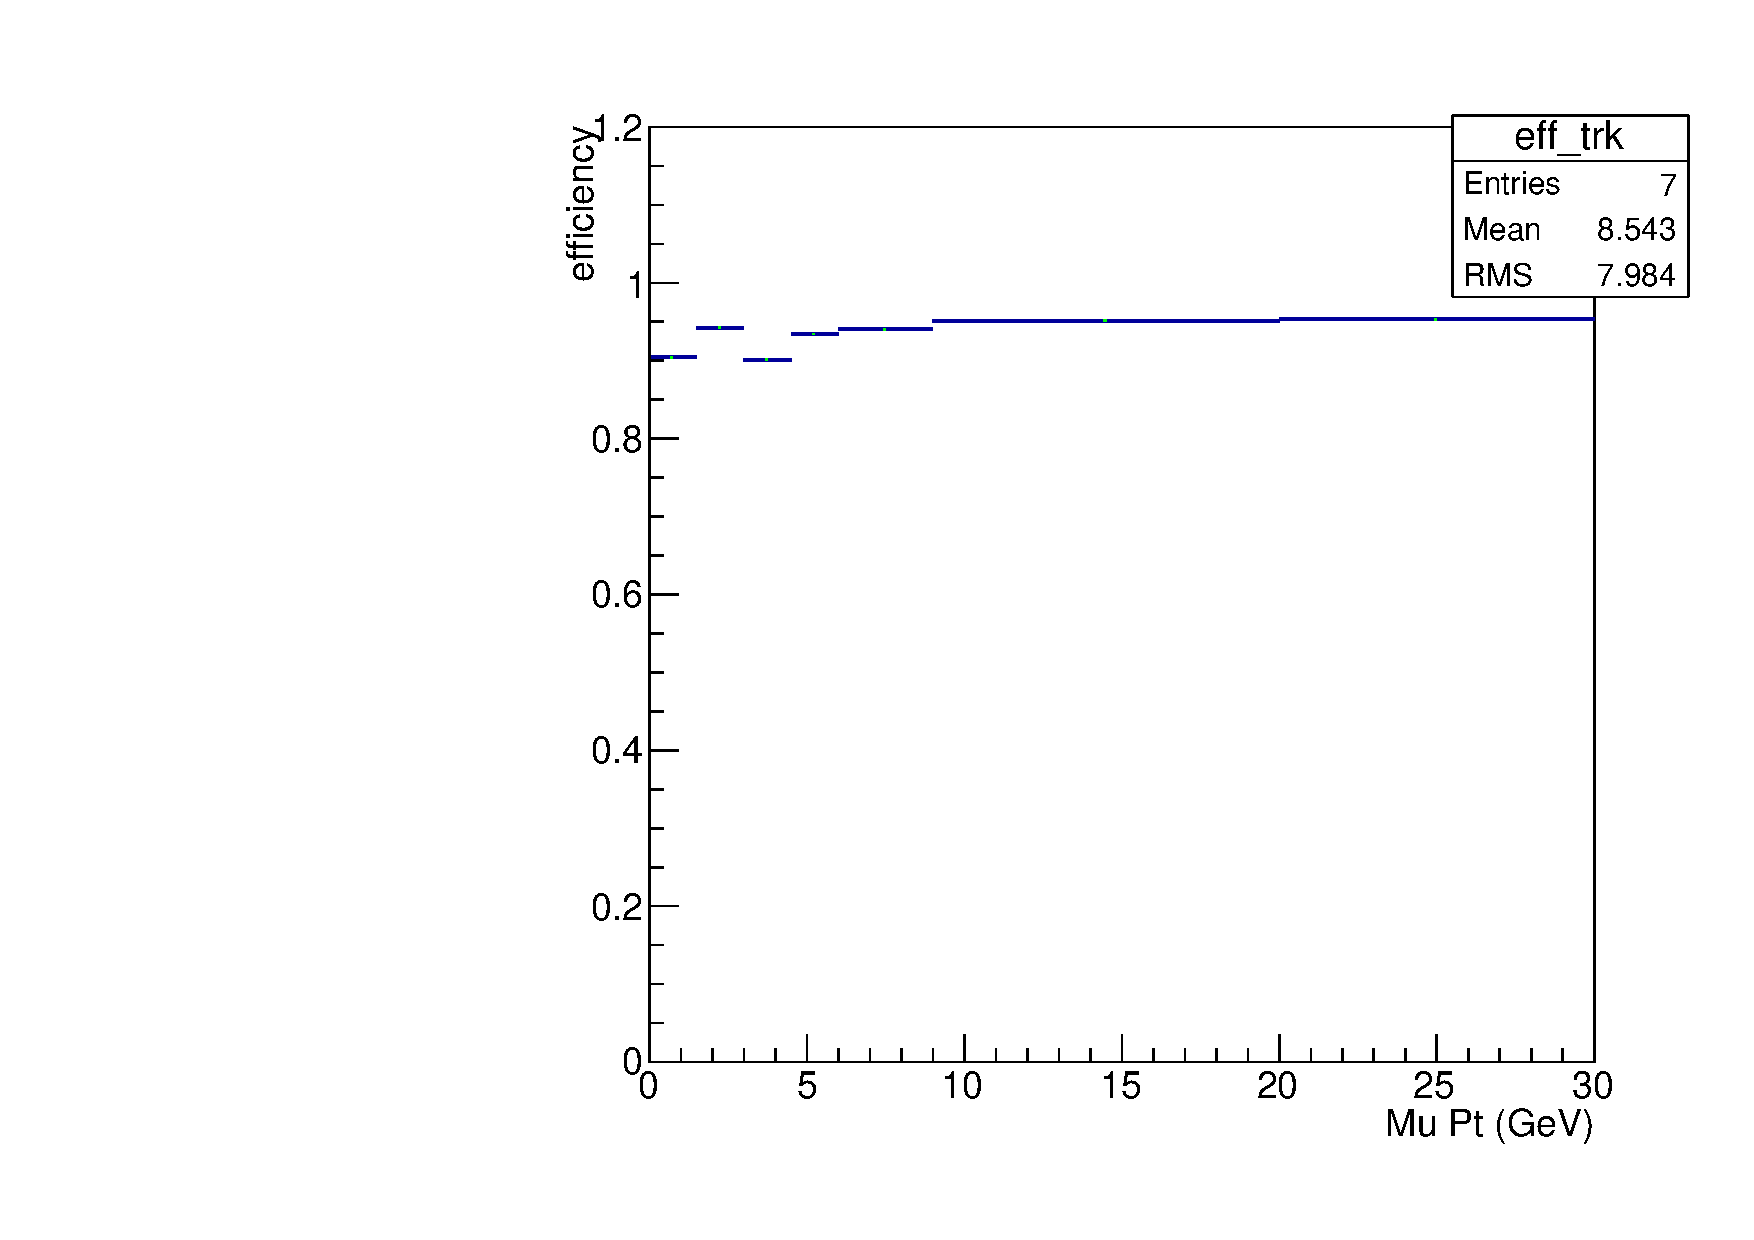
\includegraphics[width=0.25\textwidth]{../PlotsRooFitMC/eff_trk.pdf}
    \caption{MC efficiencies for Trigger(left), MuonID (centre), Tracking (right) 
    $\rm p_{t}$ (GeV/c)= {0.0-1.5}, {1.5-3.0}, {3.0-4.5}, {4.5-6.0}, {6.0-9.0}, {9.0-20.0}, {20.0-30.0}}
   % \label{simulationfigure}
\end{figure}



%--------------------------- DATA ----------------------------



\begin{figure}
    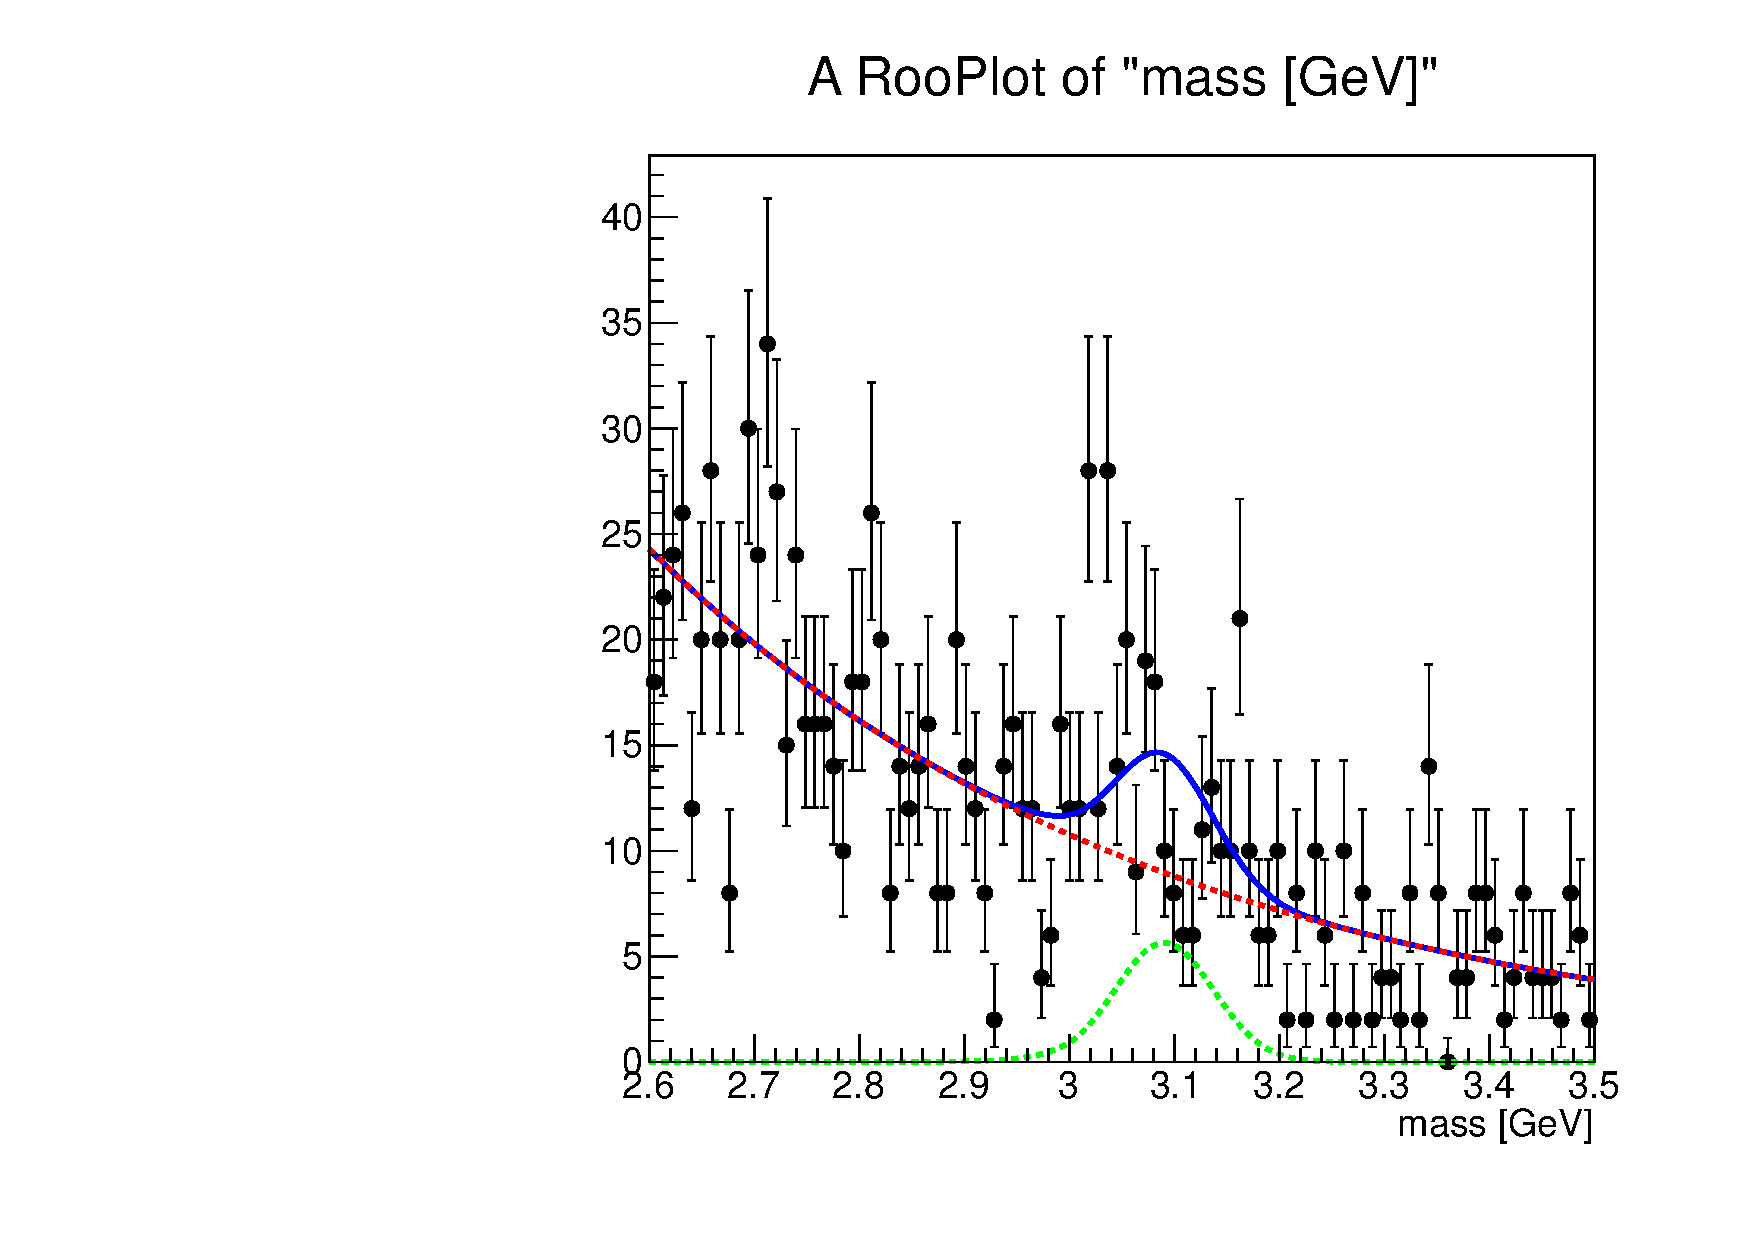
\includegraphics[width=0.25\textwidth]{../PlotsRooFitData/croofit_trg_pass_0.pdf}
    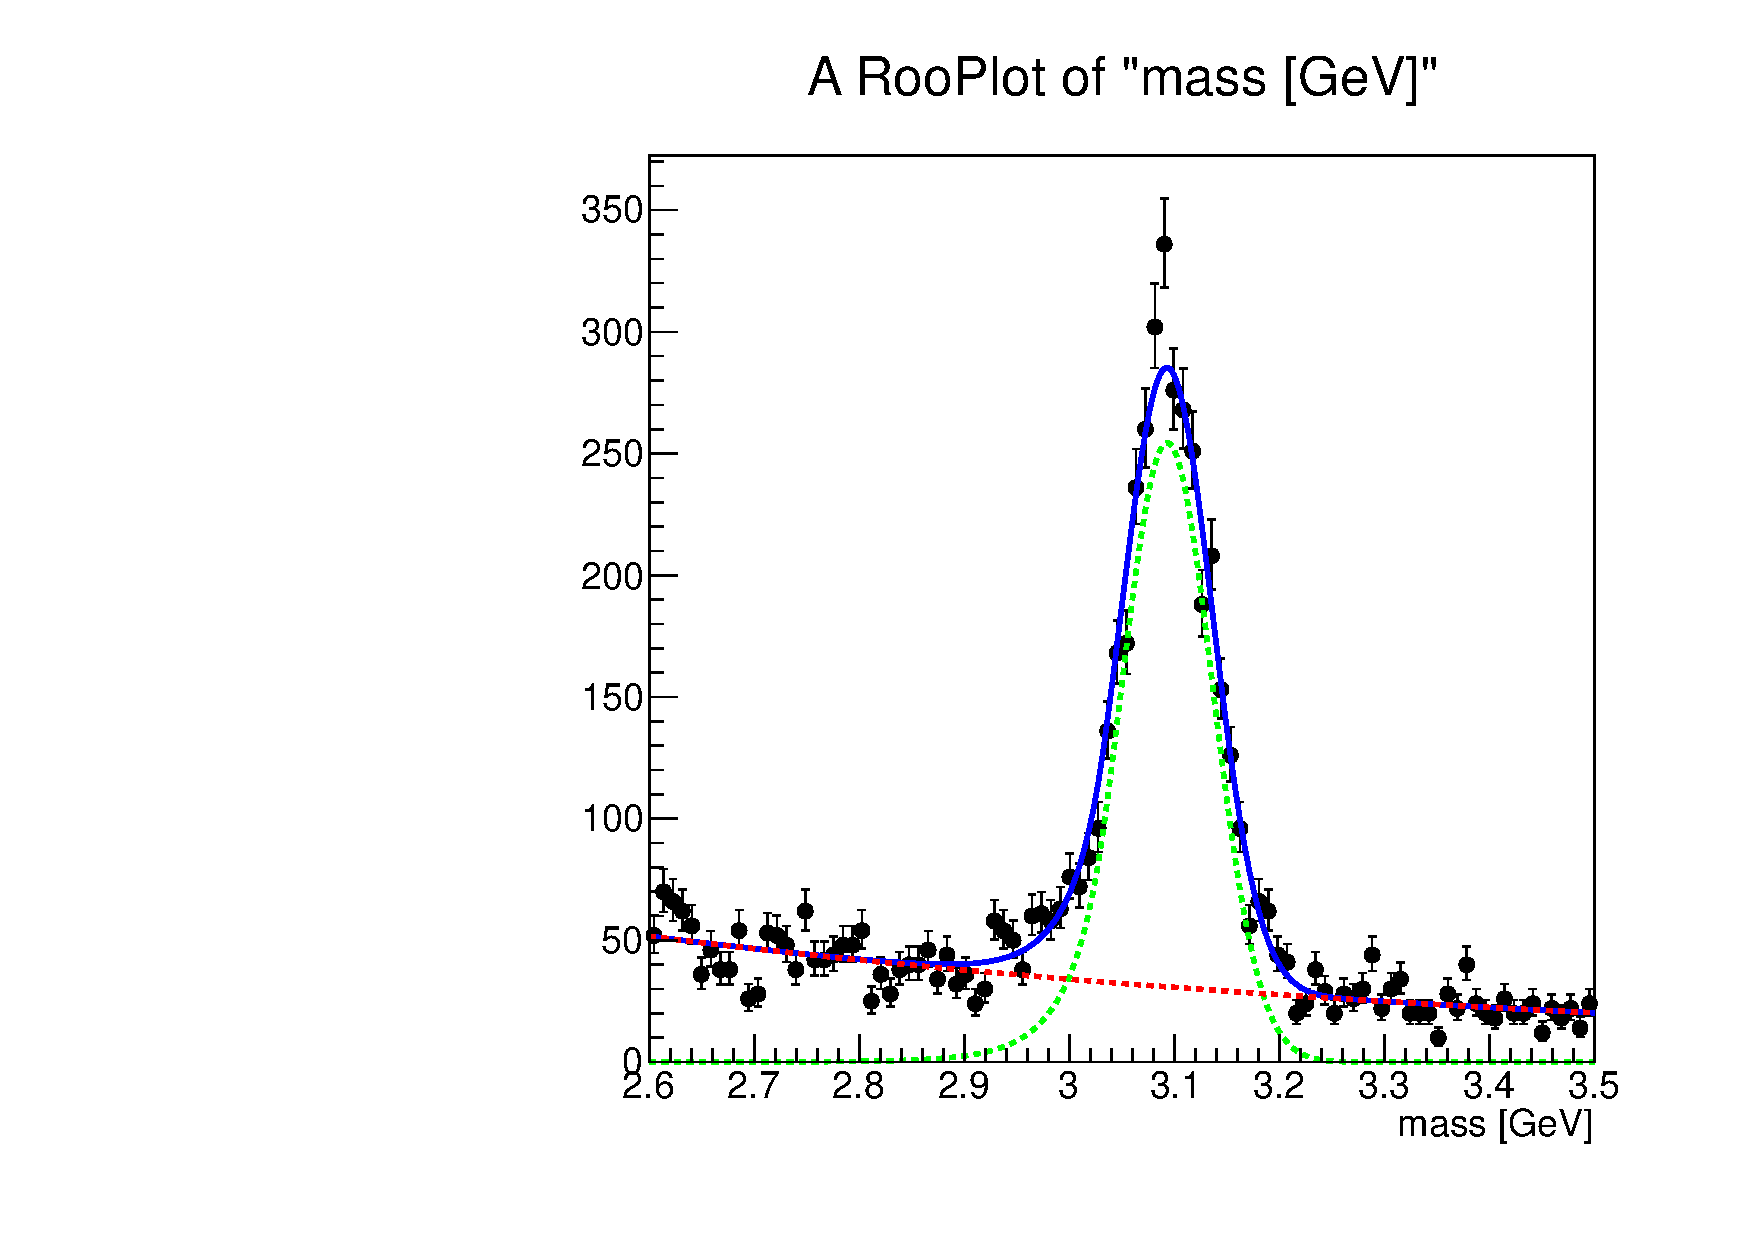
\includegraphics[width=0.25\textwidth]{../PlotsRooFitData/croofit_trg_pass_1.pdf}
    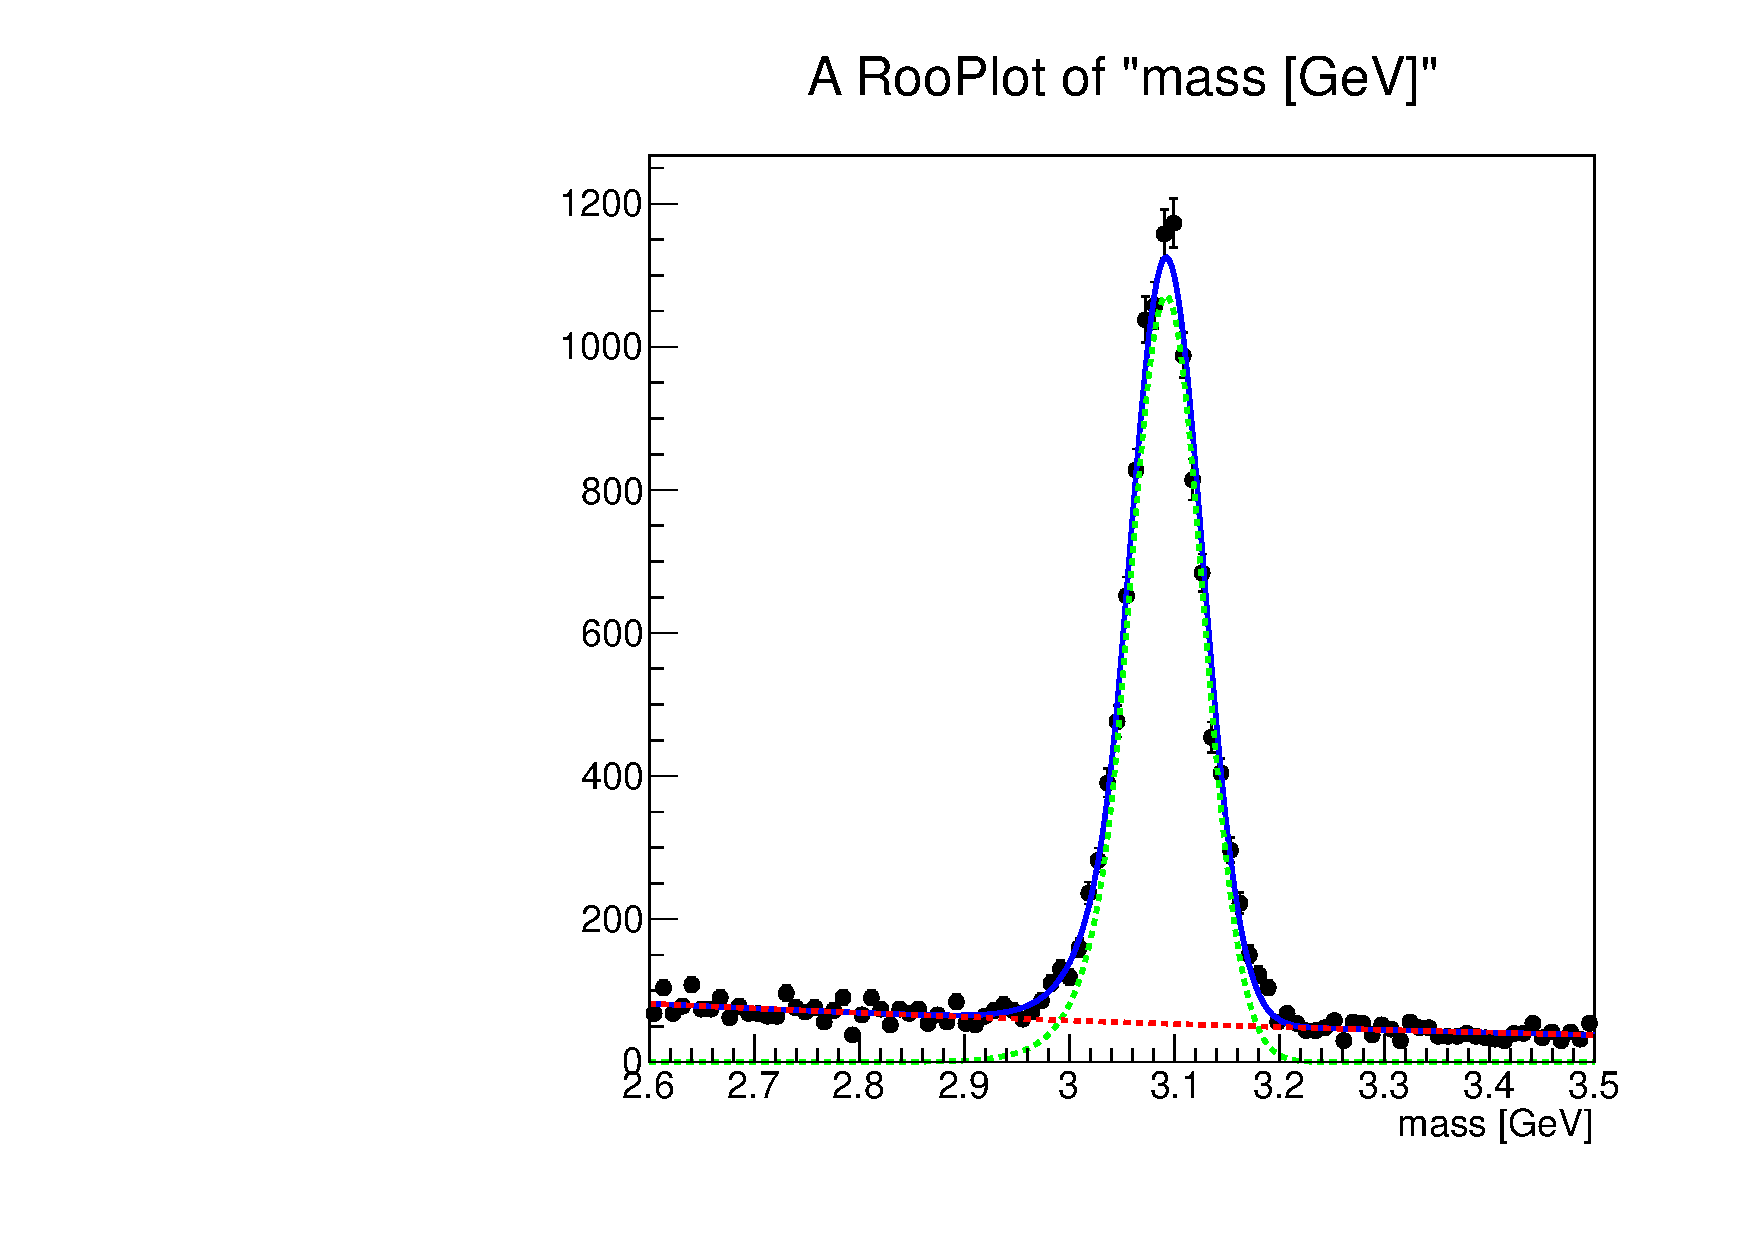
\includegraphics[width=0.25\textwidth]{../PlotsRooFitData/croofit_trg_pass_2.pdf}
    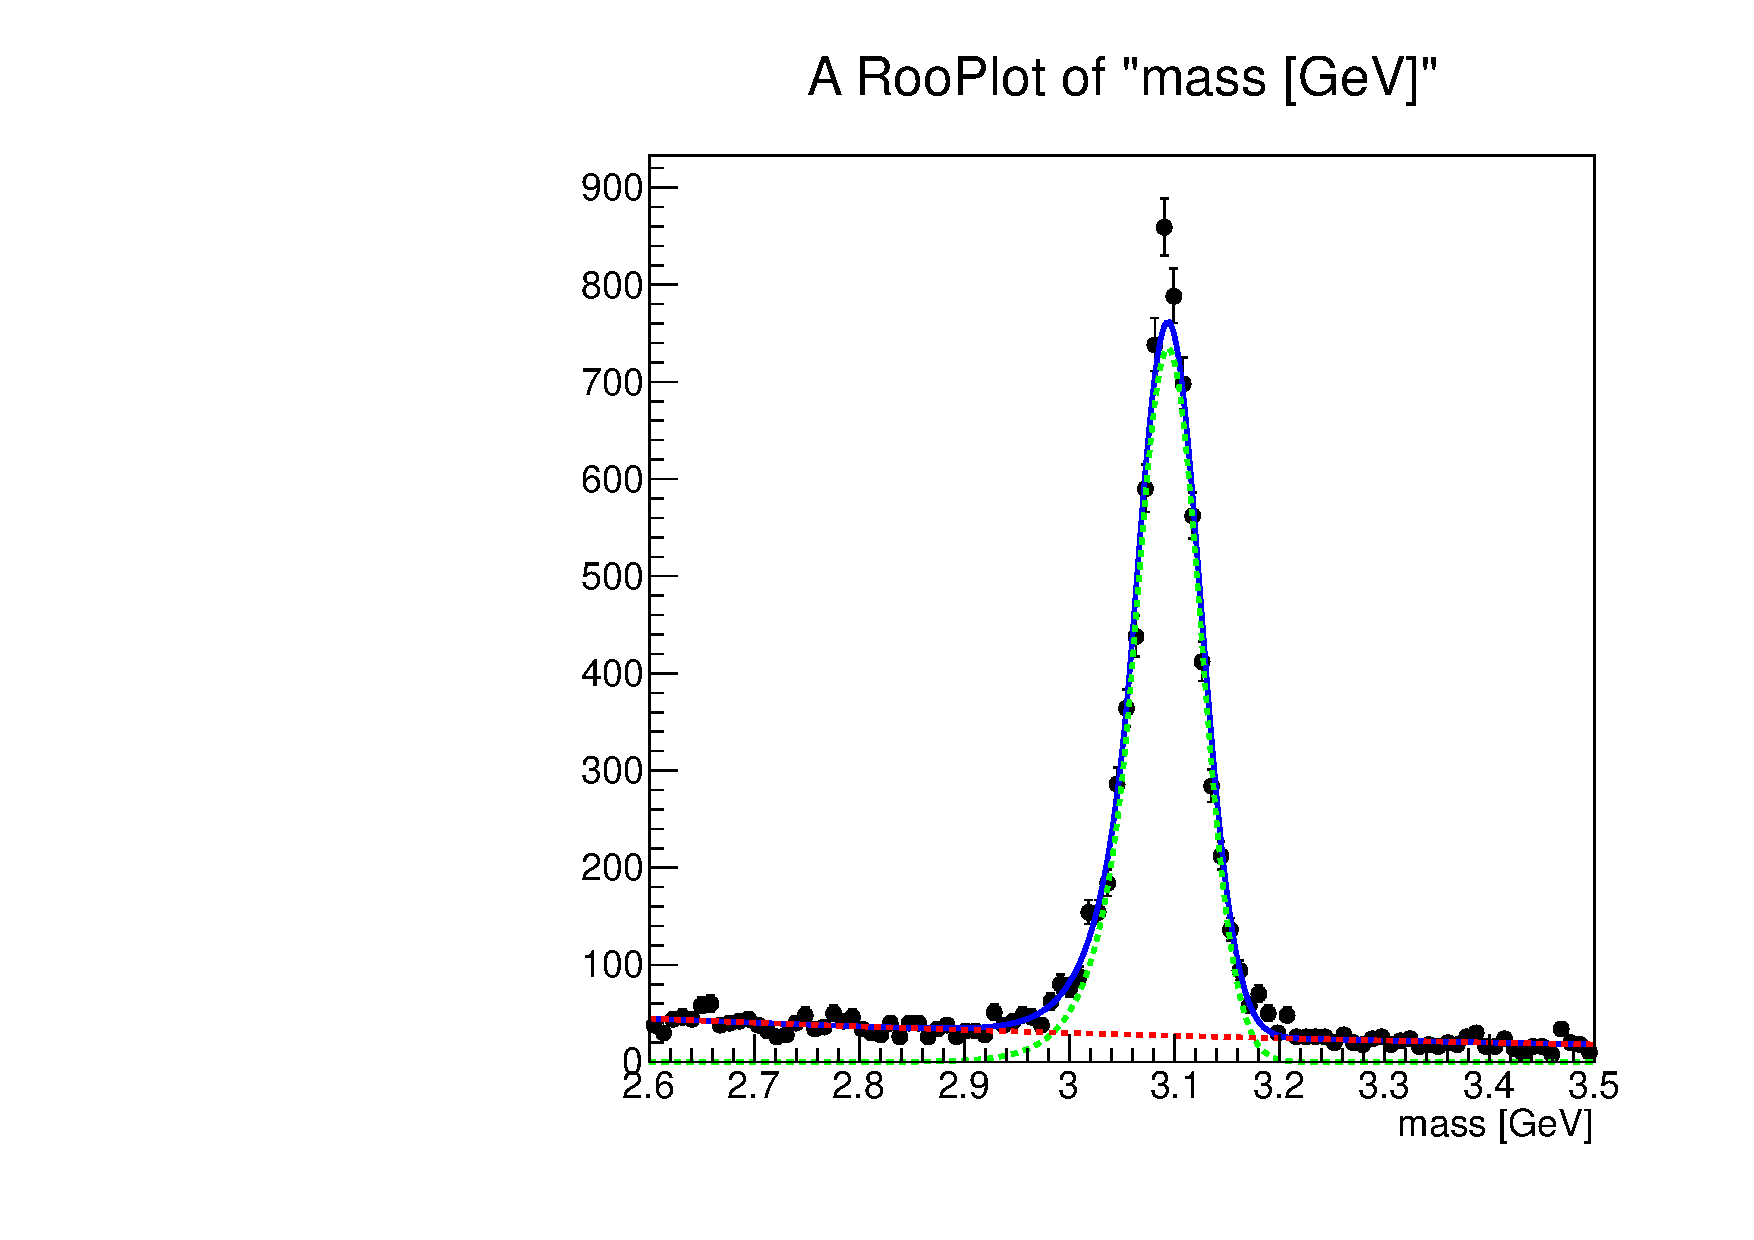
\includegraphics[width=0.25\textwidth]{../PlotsRooFitData/croofit_trg_pass_3.pdf}
    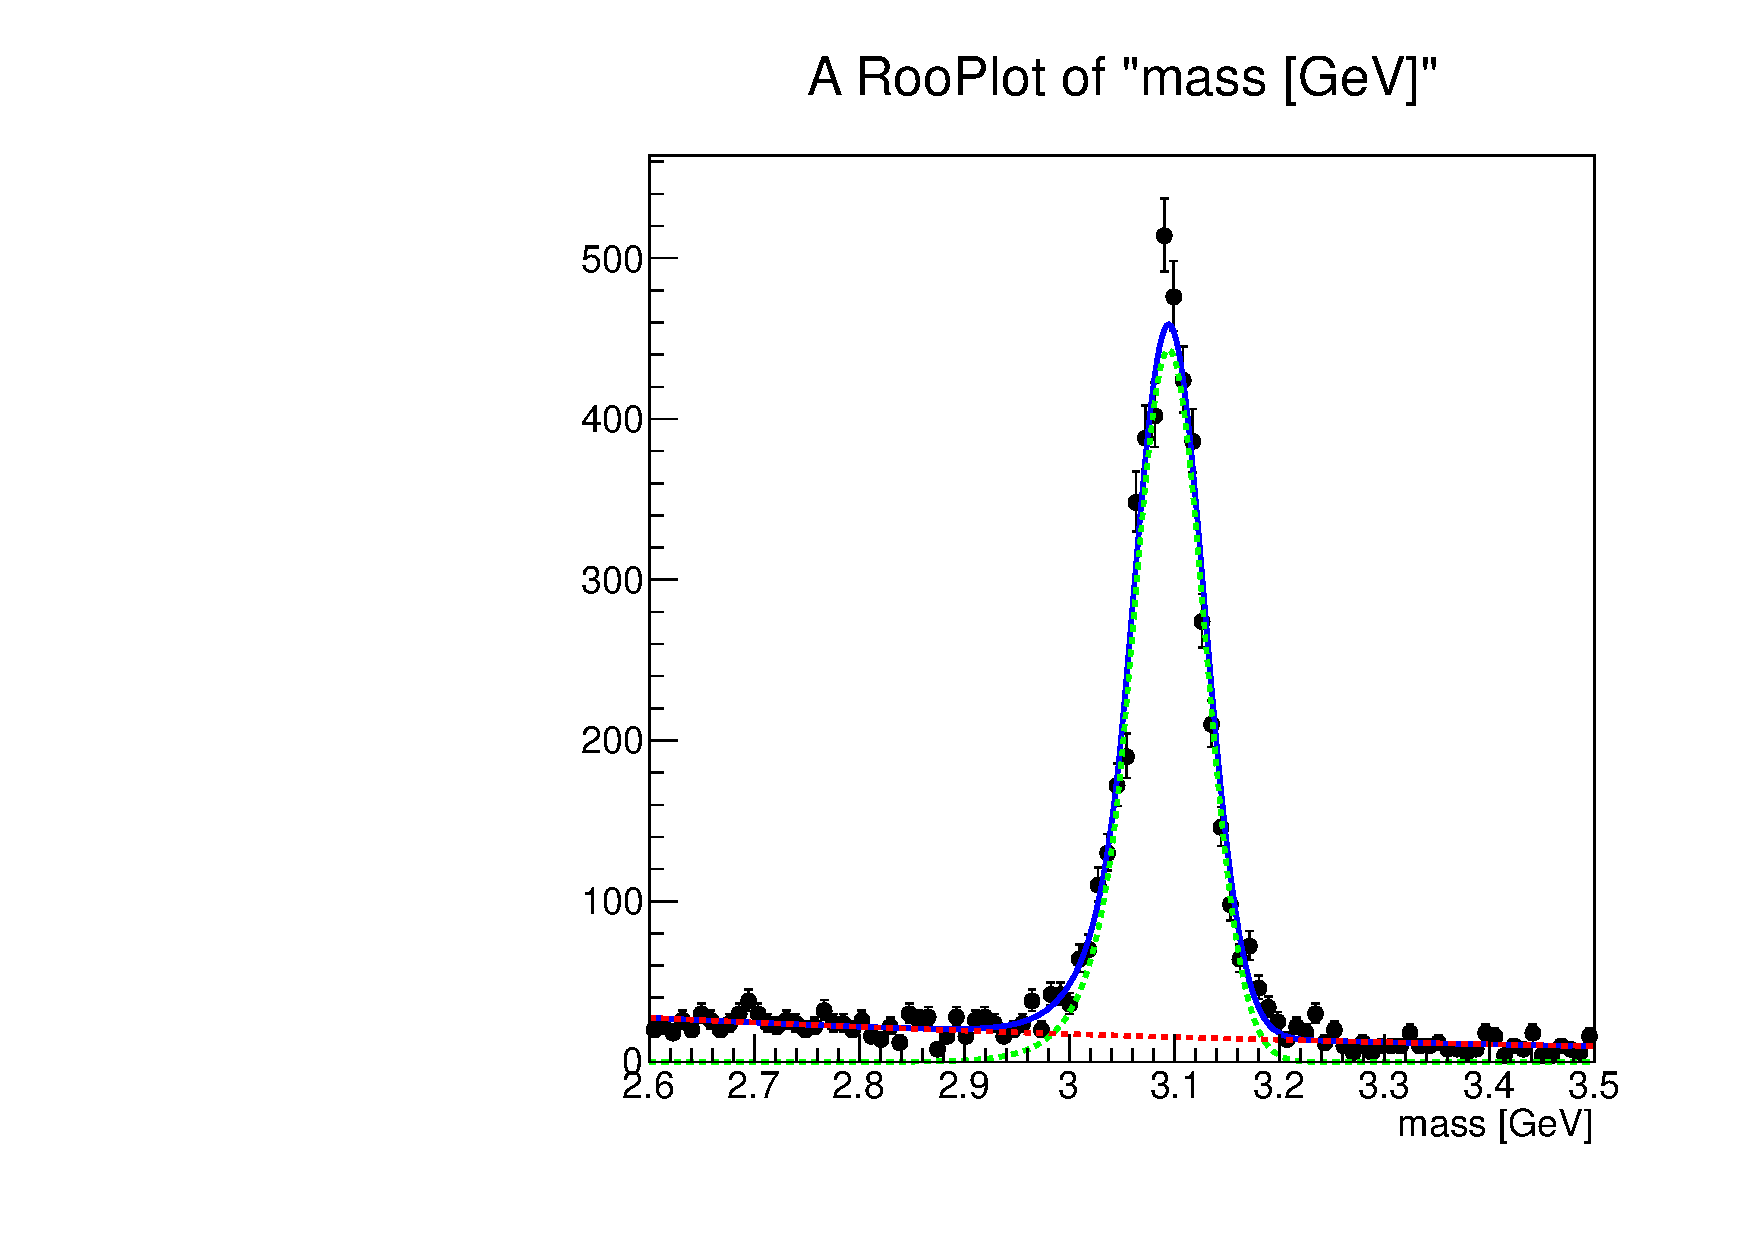
\includegraphics[width=0.25\textwidth]{../PlotsRooFitData/croofit_trg_pass_4.pdf}
    \includegraphics[width=0.25\textwidth]{../PlotsRooFitData/croofit_trg_pass_5.pdf}
    \includegraphics[width=0.25\textwidth]{../PlotsRooFitData/croofit_trg_pass_6.pdf}
    \caption{Data Results trigger studies for passing probes, muon transverse momenta
    $\rm p_{t}$ (GeV/c)= {0.0-1.5}, {1.5-3.0}, {3.0-4.5}, {4.5-6.0}, 
    {6.0-9.0}, {9.0-20.0}, {20.0-30.0}}
   % \label{simulationfigure}
\end{figure}

\begin{figure}
    \includegraphics[width=0.25\textwidth]{../PlotsRooFitData/croofit_trg_fail_0.pdf}
    \includegraphics[width=0.25\textwidth]{../PlotsRooFitData/croofit_trg_fail_1.pdf}
    \includegraphics[width=0.25\textwidth]{../PlotsRooFitData/croofit_trg_fail_2.pdf}
    \includegraphics[width=0.25\textwidth]{../PlotsRooFitData/croofit_trg_fail_3.pdf}
    \includegraphics[width=0.25\textwidth]{../PlotsRooFitData/croofit_trg_fail_4.pdf}
    \includegraphics[width=0.25\textwidth]{../PlotsRooFitData/croofit_trg_fail_5.pdf}
    \includegraphics[width=0.25\textwidth]{../PlotsRooFitData/croofit_trg_fail_6.pdf}
    \caption{Data Results trigger studies for failing probes, muon transverse momenta
    $\rm p_{t}$ (GeV/c)= {0.0-1.5}, {1.5-3.0}, {3.0-4.5}, {4.5-6.0}, 
    {6.0-9.0}, {9.0-20.0}, {20.0-30.0}}
   % \label{simulationfigure}
\end{figure}


\begin{figure}
    \includegraphics[width=0.25\textwidth]{../PlotsRooFitData/croofit_trk_pass_0.pdf}
    \includegraphics[width=0.25\textwidth]{../PlotsRooFitData/croofit_trk_pass_1.pdf}
    \includegraphics[width=0.25\textwidth]{../PlotsRooFitData/croofit_trk_pass_2.pdf}
    \includegraphics[width=0.25\textwidth]{../PlotsRooFitData/croofit_trk_pass_3.pdf}
    \includegraphics[width=0.25\textwidth]{../PlotsRooFitData/croofit_trk_pass_4.pdf}
    \includegraphics[width=0.25\textwidth]{../PlotsRooFitData/croofit_trk_pass_5.pdf}
    \includegraphics[width=0.25\textwidth]{../PlotsRooFitData/croofit_trk_pass_6.pdf}
    \caption{Data Results trigger studies for passing probes, muon transverse momenta
    $\rm p_{t}$ (GeV/c)= {0.0-1.5}, {1.5-3.0}, {3.0-4.5}, {4.5-6.0}, 
    {6.0-9.0}, {9.0-20.0}, {20.0-30.0}}
   % \label{simulationfigure}
\end{figure}

\begin{figure}
    \includegraphics[width=0.25\textwidth]{../PlotsRooFitData/croofit_trk_fail_0.pdf}
    \includegraphics[width=0.25\textwidth]{../PlotsRooFitData/croofit_trk_fail_1.pdf}
    \includegraphics[width=0.25\textwidth]{../PlotsRooFitData/croofit_trk_fail_2.pdf}
    \includegraphics[width=0.25\textwidth]{../PlotsRooFitData/croofit_trk_fail_3.pdf}
    \includegraphics[width=0.25\textwidth]{../PlotsRooFitData/croofit_trk_fail_4.pdf}
    \includegraphics[width=0.25\textwidth]{../PlotsRooFitData/croofit_trk_fail_5.pdf}
    \includegraphics[width=0.25\textwidth]{../PlotsRooFitData/croofit_trk_fail_6.pdf}
    \caption{Data Results tracking studies for failing probes, muon transverse momenta
    $\rm p_{t}$ (GeV/c)= {0.0-1.5}, {1.5-3.0}, {3.0-4.5}, {4.5-6.0}, 
    {6.0-9.0}, {9.0-20.0}, {20.0-30.0}}
   % \label{simulationfigure}
\end{figure}

\begin{figure}
    \includegraphics[width=0.25\textwidth]{../PlotsRooFitData/croofit_id_pass_0.pdf}
    \includegraphics[width=0.25\textwidth]{../PlotsRooFitData/croofit_id_pass_1.pdf}
    \includegraphics[width=0.25\textwidth]{../PlotsRooFitData/croofit_id_pass_2.pdf}
    \includegraphics[width=0.25\textwidth]{../PlotsRooFitData/croofit_id_pass_3.pdf}
    \includegraphics[width=0.25\textwidth]{../PlotsRooFitData/croofit_id_pass_4.pdf}
    \includegraphics[width=0.25\textwidth]{../PlotsRooFitData/croofit_id_pass_5.pdf}
    \includegraphics[width=0.25\textwidth]{../PlotsRooFitData/croofit_id_pass_6.pdf}
    \caption{Data Results muonID studies for passing probes, muon transverse momenta
    $\rm p_{t}$ (GeV/c)= {0.0-1.5}, {1.5-3.0}, {3.0-4.5}, {4.5-6.0}, 
    {6.0-9.0}, {9.0-20.0}, {20.0-30.0}}
   % \label{simulationfigure}
\end{figure}

\begin{figure}
    \includegraphics[width=0.25\textwidth]{../PlotsRooFitData/croofit_id_fail_0.pdf}
    \includegraphics[width=0.25\textwidth]{../PlotsRooFitData/croofit_id_fail_1.pdf}
    \includegraphics[width=0.25\textwidth]{../PlotsRooFitData/croofit_id_fail_2.pdf}
    \includegraphics[width=0.25\textwidth]{../PlotsRooFitData/croofit_id_fail_3.pdf}
    \includegraphics[width=0.25\textwidth]{../PlotsRooFitData/croofit_id_fail_4.pdf}
    \includegraphics[width=0.25\textwidth]{../PlotsRooFitData/croofit_id_fail_5.pdf}
    \includegraphics[width=0.25\textwidth]{../PlotsRooFitData/croofit_id_fail_6.pdf}
    \caption{Data Results muonID studies for failing probes, muon transverse momenta
    $\rm p_{t}$ (GeV/c)= {0.0-1.5}, {1.5-3.0}, {3.0-4.5}, {4.5-6.0}, 
    {6.0-9.0}, {9.0-20.0}, {20.0-30.0}}
   % \label{simulationfigure}
\end{figure}

\begin{figure}
    \includegraphics[width=0.25\textwidth]{../PlotsRooFitData/eff_trg.pdf}
    \includegraphics[width=0.25\textwidth]{../PlotsRooFitData/eff_id.pdf}
    \includegraphics[width=0.25\textwidth]{../PlotsRooFitData/eff_trk.pdf}
    \caption{Data efficiencies for Trigger(left), MuonID (centre), Tracking (right) 
    $\rm p_{t}$ (GeV/c)= {0.0-1.5}, {1.5-3.0}, {3.0-4.5}, {4.5-6.0}, {6.0-9.0}, {9.0-20.0}, {20.0-30.0}}
   % \label{simulationfigure}
\end{figure}



\end{document}